\documentclass[11pt,a4paper]{article}

\newcommand{\titolo}{Simulazione della rete ferroviaria Lombarda}
\newcommand{\sottotitolo}{Sviluppo del progetto Milan RailSim}
\newcommand{\autore}{Fabio Compagnoni}
\newcommand{\matricola}{944954}
\newcommand{\corso}{Sistemi Complessi: Modelli e Simulazione}
\newcommand{\corsodilaurea}{Corso di Laurea Magistrale in Informatica}
\newcommand{\ateneo}{Università degli Studi di Milano-Bicocca}
\newcommand{\dipartimento}{Dipartimento di Informatica, Sistemistica e Comunicazione}
\newcommand{\annoaccademico}{2025/2026}

% ---------------------------------------------------------------------------
% Lingua e caratteri
% ---------------------------------------------------------------------------
\usepackage[T1]{fontenc}
\usepackage[utf8]{inputenc}
\usepackage[italian]{babel}
\usepackage{lmodern}
\usepackage{microtype}
\usepackage{csquotes}
\usepackage{eurosym}

% ---------------------------------------------------------------------------
% Pagina
% ---------------------------------------------------------------------------
\usepackage[a4paper,margin=2.5cm,headheight=14pt]{geometry}
\usepackage{fancyhdr}
\pagestyle{fancy}
\fancyhf{}
\fancyhead[L]{\small\nouppercase{\leftmark}}
\fancyhead[R]{\small\autore}
\fancyfoot[C]{\thepage}
\renewcommand{\headrulewidth}{0.4pt}
\setlength{\parskip}{0.4em}

% ---------------------------------------------------------------------------
% Figure e tabelle
% ---------------------------------------------------------------------------
\usepackage{graphicx}
\graphicspath{{img/}}
\usepackage{float}
\usepackage[font=small,labelfont=bf,labelsep=period]{caption}
\usepackage{subcaption}
\usepackage{booktabs}
\usepackage{tabularx}
\usepackage{longtable}
\usepackage{xcolor}
\usepackage{tikz}
\usetikzlibrary{arrows.meta}
\usepackage{pgfplots}
\pgfplotsset{compat=1.18}

\usepackage{listings}
\renewcommand{\lstlistingname}{Listato}
\lstdefinelanguage{json}{
	string=[s]{"}{"},
	comment=[l]{//},
	morecomment=[s]{/*}{*/}
}
\lstset{
	basicstyle=\ttfamily\footnotesize,
	keywordstyle=\color{blue!50!black},
	stringstyle=\color{green!35!black},
	commentstyle=\color{gray},
	breaklines=true,
	columns=fullflexible,
	keepspaces=true,
	showstringspaces=false,
	tabsize=2,
	frame=none,
	xleftmargin=1.5em,
	captionpos=b,
	aboveskip=1em,
	belowskip=1em
}

% ---------------------------------------------------------------------------
% Numeri e unità di misura, con la virgola decimale
% ---------------------------------------------------------------------------
\usepackage{amsmath}
\usepackage{siunitx}
\sisetup{
	locale=IT,
	group-separator={\,},
	group-minimum-digits=5,
	per-mode=symbol,
	detect-all
}
\DeclareSIUnit{\euro}{\text{\euro}}
\DeclareSIUnit{\trenokm}{treno\text{-}km}
\DeclareSIUnit{\litro}{l}

\usepackage[backend=biber,style=numeric,sorting=none,maxbibnames=6]{biblatex}
\addbibresource{bibliografia.bib}

\usepackage[hidelinks]{hyperref}
\usepackage[italian,nameinlink]{cleveref}
\crefname{listing}{listato}{listati}
\Crefname{listing}{Listato}{Listati}
\hypersetup{pdftitle={\titolo},pdfauthor={\autore}}

\begin{document}

% ---------------------------------------------------------------------------
% Frontespizio
% ---------------------------------------------------------------------------
\begin{titlepage}
	\centering
	{\large\textsc{\ateneo}\par}
	\vspace{0.3cm}
	{\dipartimento\par}
	{\corsodilaurea\par}
	\vfill
	\IfFileExists{img/logo_extended.pdf}{%
		
\includegraphics[width=0.75\textwidth]{logo_extended.pdf}\par
	}{}
	\vspace{1.5cm}
	{\LARGE\bfseries\titolo\par}
	\vspace{0.6cm}
	{\large\sottotitolo\par}
	\vspace{0.3cm}
	{\large Corso di \emph{\corso}\par}
	\vfill
	\begin{flushright}
		\autore\\
		Matricola \matricola
	\end{flushright}
	\vspace{1cm}
	{Anno accademico \annoaccademico\par}
\end{titlepage}

\begin{abstract}
Il lavoro studia, con un modello di simulazione, quanto si possa aumentare la frequenza dei treni regionali e suburbani della Lombardia senza apportare modifiche alll'infrastruttura esistente, e quali punti della rete siano il limite per questo obiettivo.\\
Il servizio è modellato come un sistema multi-agente modellato tramite un grafo. L'ambiente corrisponde alla rete, descritta sia in modo mesoscopico che microscopico a seconda del livello necessario. Gli agenti sono i treni, reattivi ed eterogenei per prestazioni, e interagiscono solo in modo indiretto, contendendosi i binari: ritardi, code e blocchi non sono scritti in alcuna regola ed emergono da questa interazione.\\
Il modello è deterministico e non non sono stati considerati i passeggeri come agenti del sistema ma come massa trasportata dai treni. La rete, l'assegnazione dei treni alle corse e ai binari e le regole di precedenza nelle stazioni e sul binario unico sono state ricavate da dati pubblici. Ogni simulazione calcola puntualità, consumi e costi. Il modello è stato validato sull'orario reale di un'intera settimana: tutte le corse sono completate, i tempi di percorrenza si discostano di meno dell'1\% dall'orario, l'energia di pochi punti percentuali dai dati pubblicati, e la puntualità, 94\%, è un limite superiore di quella reale. Due gruppi di scenari aumentano le corse. Il servizio può crescere solo in modo localizzato: un'attesa massima di 10 minuti sui tratti urbani richiede 33 treni e il 6\% di costi in più e riduce la puntualità di 2,4 punti.\\
I limiti sono il binario unico, che porta al 66\% la puntualità della linea S9, e il tunnel del Passante e i nodi attorno a Milano, dove un aumento diffuso riduce le corse completate anche sulle linee non potenziate.
\end{abstract}

\tableofcontents
\clearpage
% Contentuo %

\section{Introduzione}
\subsection{Contesto}
Il contesto in cui si inserisce il progetto \textit{Milan RailSim} è quello della simulazione della rete ferroviaria lombarda, in particolare la rete suburbana e il passante milanese. \\
L'obiettivo del progetto è la simulazione del traffico ferroviario, del comportamento dei treni e della gestione delle stazioni, al fine di analizzare l'efficienza del sistema e identificare eventuali criticità.\\
L'obiettivo principale è quello di analizare le reti suburbane e cercare di analizzare se sia possibile avere un comportamente più simile ad una metropolitana piuttosto che ad un sistema ferroviario, dunque simulare se fosse possibile aumentare il numero di corse e ridurre l'attesa, senza modificare l'infrastruttura già esistente.\\
Dato che sulla stessa infrastruttura circolano, insieme ai suburbani, anche i treni regionali e treni di altre società, non è possibile simulare solamente il comportamento dei suburbani, in quanto non sarebbe corretto: è stata quindi simulata l'intera rete regionale di Trenord. I treni delle altre società, come quelli a lunga percorrenza e ad alta velocità, usano in parte gli stessi binari ma non sono rappresentati nel modello.\\
Il punto più delicato della rete è il Passante ferroviario, una galleria a due binari che attraversa la città e nella quale confluiscono sei linee suburbane. Nell'orario in vigore vi transitano 12 treni all'ora per verso, con intervalli irregolari che vanno da 2 a oltre 9 minuti.\\
Un altro problema che è stato necessario modellare è la presenza di binari unici, dunque tratti di binario utilizzate in entrambi i versi, dunque per mantenere realistico il modello è stato necessario modellare anche questo comportamento.\\

\subsection{Motivazione}
\'E stato scelto di simulare questo caso d'uso, sia per un interesse personale, in quanto da pendolare vivo tutti i giorni le problematiche dei treni in Lombardia, sia per un interesse accademico, in quanto la rete ferroviaria lombarda è un esempio di sistema complesso, in cui il comportamento dell'intero sistema non si ricava dalle regole dei singoli treni, ma dal comportamento collettivo dei treni e dalle interazioni tra di essi.\\

\subsection{Domanda di ricerca e obiettivi}
La domanda da cui parte il lavoro è la seguente: di quanto si può aumentare la frequenza dei treni prima che i ritardi si propaghino a tutta la rete, e quali punti dell'infrastruttura fissano questo limite?

L'obiettivo non è trovare l'orario migliore.
L'obiettivo è comprendere come il sistema reale si comporta e come potrebbe comportarsi in scenari alternativi.
Gli obiettivi da raggiungere sono quattro:
\begin{itemize}
	\item costruire un modello di base utilizzando la rete reale e gli orari ufficiali del servizio, cercando di modellare un sistema realistico
	\item implementazione di uno scenario in cui la rete suburbana ha un aumento delle corse mentre il resto della rete rimane invariato;
	\item implementazione di uno scenario più irrealistico dei primi due, in cui tutta la rete subisce un aumento delle corse e di riduzione dei tempi di attesa, con l'obiettivo di ricercare i colli di bottiglia e dove la rete si satura più velocemente;
	\item per ogni scenario, stimare i costi i costi di servizio, come il costo per la trazione, del personale, ecc...
\end{itemize}

\subsection{Che cosa è stato realizzato}

La simulazione si basa su \textit{railsim}~\cite{kaddoura2024railsim}, un'estensione ferroviaria della piattaforma di simulazione ad agenti MATSim. I dettagli di ogni parte verranno specificati nelle sezioni dedicate.\\

Da railsim sono stati usati:
\begin{itemize}
	\item il motore di simulazione, che fa avanzare i treni sulla rete secondo per secondo;
	\item il moto dei treni, con accelerazione, frenata e velocità massima proprie di ogni tipo di treno;
	\item l'occupazione dei binari: un treno entra in una tratta solo se è libera, altrimenti attende;
	\item la rappresentazione di una tratta a binario unico come risorsa condivisa dai due versi di marcia;
	\item la possibilità di deviare un treno su un altro binario della stessa stazione;
	\item i punti di estensione, attraverso i quali sono state inserite le regole aggiuntive.
\end{itemize}

Per il progetto sono stati sviluppati:
\begin{itemize}
	\item la costruzione della rete a partire dall'orario pubblico di Trenord e dai dati di OpenStreetMap;
	\item le stazioni principali, con specifica di dettaglio a livello di binario, con gli ingressi, le uscite e i binari di ricovero;
	\item il caricamento delle corse dall'orario pubblico e la loro assegnazione ai treni e ai binari, informazioni che l'orario non contiene;
	\item le regole per gli incroci sul binario unico, che stabiliscono quando un treno può entrare in una tratta e dove attende il treno opposto;
	\item la misura della puntualità, il calcolo del consumo di energia e il calcolo dei costi, che railsim non prevede;
	\item i generatori degli scenari, che aggiungono corse all'orario reale;
	\item un'applicazione grafica che mostra i treni sulla mappa durante la simulazione, archivia ogni simulazione e ne presenta i risultati in tabelle e grafici.
\end{itemize}

\subsection{Metodo di lavoro}
La realizzazione del progetto è stata guidata dai dati ottenuti dalla simulazioni e dal confronto con i dati reali.\\
Lo sviluppo è stato TDD (Test Driven Development), ovvero prima della scrittura del codice sono state scritte le suite di test e i test unitari che doveno passare una volta implementata la funzionalità.\\
Al termine dello sviluppo veniva eseguito lo scenario di simulazione su una giornata completa, per verificare se il comportamento era corretto o si verificano situazioni anomale.\\
Per lo sviluppo del codice e l'esecuzione dei test è stato è stato d'aiuto \textit{Claude Code}, l'assistente di programmazione di Anthropic, con i modelli Opus 5.5 e Fable 5.1.

\section{Strumenti e alternative}
\subsection{Scelta dello strumento}
% BOZZA: testo di partenza, da rivedere e riscrivere.
Per rispondere alla domanda di ricerca serviva uno strumento in grado di simulare un'intera rete regionale, con centinaia di treni al giorno, e al tempo stesso di rappresentare con precisione i punti in cui la capacità è limitata: i nodi, le stazioni principali e le tratte a binario unico. 
Doveva inoltre permettere di modificare le regole con cui i treni si contendono i binari, perché sono queste regole a determinare come i ritardi si propagano.\\

Gli strumenti professionali più diffusi, come OpenTrack e Trenissimo, simulano la circolazione su una descrizione dettagliata dei binari. Gli autori di railsim ne indicano però i limiti~\cite{kaddoura2024railsim}: il codice è chiuso e non può essere esaminato né modificato, le possibilità di estensione sono ridotte, non è possibile inserire regole proprie per la gestione della circolazione, e l'approccio esclusivamente microscopico richiede dati molto dettagliati su binari e itinerari, il che rende onerosa la simulazione di una rete regionale o nazionale. \\
Esiste anche un simulatore a codice aperto, Flatland, anch'esso microscopico, che usa però una rappresentazione semplificata della realtà ed è impiegato soprattutto per studiare strategie di controllo dei treni con tecniche di apprendimento automatico~\cite{kaddoura2024railsim}. 
All'estremo opposto si trova MATSim usato senza estensioni, che simula il trasporto pubblico a orario ma in cui i veicoli seguono l'orario senza interagire fra loro, e quindi non rappresenta l'esercizio ferroviario~\cite{kaddoura2024railsim}.\\

L'idea iniziale del progetto era lo sviluppo di un simulatore da zero, ma l'idea è stata abbandonata perchè il settore ferroviario comprende molti aspetti legati fra loro, dal moto dei treni all'occupazione dei binari, dalle stazioni agli incroci, e una implementazione scritta da zero non avrebbe raggiunto, nei tempi disponibili, un risultato realistico.\\
% BOZZA: frase su Mesa, da rivedere e riscrivere.
Fra le alternative, c'era anche Mesa~\cite{terhoeven2025mesa}, una libreria Python a codice aperto per la modellazione ad agenti. Mesa fornisce gli elementi generali di un modello ad agenti, ma nessun componente ferroviario: rete, moto dei treni, occupazione dei binari e gestione dell'orario sarebbero stati da scrivere per intero, con le stesse difficoltà dello sviluppo da zero, ma con i vincoli di utilizzare gli elementi della libreria.\\

In seguito ad un analisi di implementazioni in Railsim e la lettura della documentazione, è stato deciso di utilizzare Railsim. \\
Essendo scritto in Java ed open source, può essere esteso con implementazioni specifiche di alcuni comportamenti. Consente di descrivere la stessa rete a livello mesoscopico, microscopico o misto, e quindi di simulare una rete regionale riservando il dettaglio ai punti in cui serve. \\
Infine è sviluppato dalle Ferrovie Federali Svizzere (SBB CHF), il che ne garantisce la serietà del progetto e le sue potenzialità.\\

Lo strumento ha anche due limiti, noti fin dall'inizio. È recente e poco documentato, tanto che per conoscerne il comportamento è stato necessario leggerne il sorgente. Inoltre non costruisce la rete e non stabilisce il livello di dettaglio, che restano a carico di chi lo usa.\\
Nel progetto la rete è stata generata prima a livello mesoscopico, e poi i nodi e i punti più delicati sono stati in seguito descritti a livello microscopico, come illustrato nelle sezioni successive.

\subsection{MATSim}
% BOZZA: testo di partenza, da rivedere e riscrivere.
MATSim (\textit{Multi-Agent Transport Simulation}) è un ambiente di simulazione ad agenti per i sistemi di trasporto, scritto in Java e distribuito con licenza libera~\cite{horni2016matsim}. Il progetto nasce alla fine degli anni Novanta dal lavoro di Kai Nagel, allora al Politecnico federale di Zurigo, a cui si è unito Kay W. Axhausen. È pensato per scenari di grande scala, con milioni di agenti, e per questo ogni suo modello è ridotto all'essenziale.

In MATSim ogni persona della popolazione studiata è un agente, e ogni agente possiede un \textit{piano}: la sequenza delle attività di una giornata e degli spostamenti che le collegano, ognuno con orario, mezzo e percorso. L'unità di analisi è la giornata singola. La domanda di trasporto non è quindi assegnata come flusso fra zone, ma emerge dalla somma dei piani dei singoli agenti.

Una esecuzione è composta da un numero configurabile di iterazioni, ognuna divisa in tre fasi~\cite{horni2016matsim}. Nella prima, la simulazione della mobilità (\textit{mobsim}), tutti i piani scelti vengono eseguiti insieme sulla rete e gli agenti competono per lo spazio disponibile. Nella seconda, la valutazione (\textit{scoring}), ogni piano eseguito riceve un punteggio, che cresce con il tempo dedicato alle attività e diminuisce con il tempo di viaggio e con i ritardi; la funzione usata di norma è quella di Charypar e Nagel~\cite{charypar2005generating}. Nella terza, la ripianificazione (\textit{replanning}), una parte degli agenti, spesso il 10\%, copia il piano scelto e ne modifica un aspetto, come l'orario di partenza, il percorso o il mezzo, mentre gli altri scelgono fra i piani già in memoria in base al punteggio. Ogni agente conserva un numero limitato di piani, cinque nella configurazione predefinita, e scarta quello con il punteggio peggiore. Il ciclo si ripete finché il punteggio medio della popolazione si stabilizza. Si tratta di un algoritmo co-evolutivo: ogni agente migliora i propri piani mentre tutti gli altri fanno lo stesso, e il sistema tende a un equilibrio in cui nessuno può migliorare cambiando da solo il proprio piano.

Il motore di simulazione predefinito, chiamato QSim, usa un modello a code~\cite{gawron1998iterative} e avanza a passi di tempo fissi, di un secondo nella configurazione predefinita. La rete è un grafo orientato di nodi e collegamenti (\textit{link}). Ogni link è una coda in cui il primo veicolo entrato è il primo a uscire, ed è descritto da tre grandezze: il tempo di percorrenza a velocità libera, la capacità di deflusso, cioè quanti veicoli possono uscire nell'unità di tempo, e la capacità di accumulo, cioè quanti veicoli il link può contenere. Un veicolo lascia un link solo quando è trascorso il tempo di percorrenza a velocità libera, la capacità di deflusso del passo corrente non è esaurita e il link successivo ha spazio. Il modello non rappresenta la posizione del veicolo lungo il link, né l'accelerazione, la frenata o la distanza dal veicolo che precede: è il prezzo pagato per poter simulare scenari molto grandi.

Ogni azione che avviene nella simulazione produce un \textit{evento} con il suo istante: un agente parte, un veicolo entra in un link o ne esce, un'attività inizia. Gli eventi sono l'unico risultato grezzo della simulazione, e ogni misura, dai tempi di viaggio ai ritardi, si ottiene elaborandoli. I dati di ingresso di uno scenario minimo sono tre file in formato XML: la configurazione, la rete e la popolazione con i piani iniziali.

Il supporto al trasporto pubblico è stato aggiunto in un secondo momento~\cite{rieser2010adding} e richiede due file ulteriori. Il primo è l'orario (\textit{transit schedule}), che contiene le fermate, ognuna associata a un solo link della rete, e le linee. Ogni linea ha uno o più percorsi, e ogni percorso elenca i link attraversati, le fermate servite, con i tempi di arrivo e di partenza espressi come scarto dalla partenza iniziale, e le singole corse, ognuna con il proprio orario e il veicolo che la effettua. Il secondo file descrive i veicoli e i loro tipi, con capienza, lunghezza e velocità massima. Lo stesso veicolo può essere assegnato a più corse. Durante la simulazione ogni veicolo è guidato da un agente conducente e percorre i link della rete come gli altri veicoli, fermandosi alle fermate per far salire e scendere i passeggeri.

MATSim è costruito come un insieme di moduli sostituibili, collegati fra loro con un meccanismo di iniezione delle dipendenze: chi lo estende può sostituire un componente con una propria implementazione senza modificare il codice esistente. Le estensioni mantenute insieme al nucleo sono chiamate \textit{contrib}, e railsim è una di queste.

Il modello a code è nato per il traffico stradale. Applicato ai treni, non rappresenta ciò che determina la capacità di una ferrovia: l'uso esclusivo di un binario, la distanza di sicurezza fra due treni, i tempi di accelerazione e di frenata, l'incrocio sul binario unico. Per questo railsim sostituisce, per i soli treni, il modo in cui i veicoli si muovono sulla rete, lasciando invariato tutto il resto di MATSim~\cite{kaddoura2024railsim}.

\subsection{Railsim}
Come anticipato nell'introduzione, per l'implementazione del modello, il lavoro si è basato sull'utilizzo di \textit{railsim}~\cite{kaddoura2024railsim}, un'estensione ferroviaria della piattaforma di simulazione ad agenti MATSim.\\
% BOZZA da qui in poi: testo di partenza, da rivedere e riscrivere.

\subsubsection{Obiettivi}
Gli scopi dichiarati di railsim sono tre: verificare se un orario è eseguibile su una data infrastruttura, individuare conflitti e colli di bottiglia, e fare da base per lo studio delle perturbazioni e delle strategie di gestione della circolazione~\cite{kaddoura2024railsim}. 

\subsubsection{Integrazione con MATSim}
railsim non modifica il nucleo di MATSim: aggiunge al motore QSim un motore proprio, che prende in carico i veicoli di un modo di trasporto prefissato, per impostazione predefinita \texttt{rail}. Questi veicoli sono esclusi dal modello a code e si muovono secondo le regole di railsim; tutto il resto resta invariato~\cite{kaddoura2024railsim}. \\
I treni sono quindi veicoli del trasporto pubblico di MATSim: le corse, le fermate, i tempi e il veicolo assegnato a ogni corsa sono letti dall'orario, e ogni treno è guidato da un agente conducente, che railsim sostituisce con una propria versione. 
Lo stesso veicolo può effettuare più corse nella giornata e in questo caso resta sulla rete fra una corsa e la successiva.\\

Tre caratteristiche distinguono il moto di un treno da quello di un veicolo stradale. La prima è l'estensione nello spazio: un treno può occupare più link contemporaneamente, con la testa su uno e la coda su un altro, e un link torna disponibile solo dopo il passaggio della coda. La seconda è la dinamica: il tempo di percorrenza di un link non è fisso, ma dipende dall'accelerazione e dalla frenata del treno. La terza è la prenotazione: un treno può avanzare solo sui tratti di infrastruttura che gli sono stati assegnati, e due treni non possono ottenere lo stesso tratto.

\subsubsection{Infrastruttura: link e risorse}
La rete resta quella di MATSim, un grafo di nodi e link a senso unico, ma gli attributi stradali di capacità e numero di corsie non vengono usati. La velocità massima di un link è l'attributo ordinario di velocità libera; gli altri dati sono attributi propri di railsim, riassunti nella \cref{tab:railsim-link}.

\begin{table}[H]
	\centering
	\caption{Attributi dei link usati da railsim.}
	\label{tab:railsim-link}
	\begin{tabularx}{\textwidth}{lX}
		\toprule
		Attributo & Significato \\
		\midrule
		\texttt{railsimTrainCapacity} & Numero di treni che possono trovarsi insieme sul link. Se manca vale 1. \\
		\texttt{railsimResourceId} & Identificativo della risorsa a cui il link appartiene. I link con lo stesso identificativo si prenotano insieme. \\
		\texttt{railsimMinimumTime} & Tempo minimo fra due treni successivi sul deviatoio alla fine del link. Se manca vale 0. \\
		\texttt{railsimEntry} & Link di ingresso di una stazione: qui il treno può chiedere un percorso alternativo. \\
		\texttt{railsimExit} & Link di uscita di una stazione: è la destinazione del percorso alternativo. \\
		\bottomrule
	\end{tabularx}
\end{table}

Gli attributi si scrivono dentro l'elemento del link, nel file della rete. Il \cref{lst:railsim-capacita} mostra un link che può contenere tre treni insieme.

\begin{lstlisting}[language=XML,caption={Link con capienza di tre treni.},label={lst:railsim-capacita}]
<link id="A" from="A" to="A0" length="500" freespeed="2.77"
      capacity="3600.0" permlanes="1" oneway="1" modes="rail">
  <attributes>
    <attribute name="railsimTrainCapacity"
               class="java.lang.Integer">3</attribute>
  </attributes>
</link>
\end{lstlisting}

Il concetto centrale è quello di \textit{risorsa}. La capacità non è una proprietà del singolo link ma della risorsa, che è formata da uno o più link e ha una capienza pari alla minima fra quelle dei suoi link; un link senza identificativo è una risorsa a sé. Con le risorse si descrivono le situazioni tipiche della ferrovia. Un binario percorribile nei due sensi è una coppia di link di verso opposto con la stessa risorsa: un treno che ne occupa uno blocca anche l'altro. Una sezione di blocco fisso è una sequenza di link con la stessa risorsa e capienza 1. Il blocco mobile si ottiene con link corti, ognuno con la propria risorsa. Un'intersezione fra due binari è protetta dal nodo comune, che resta bloccato finché un treno lo impegna.

Il \cref{lst:railsim-binario-unico} mostra il caso del binario unico: due link di verso opposto fra gli stessi nodi, con lo stesso identificativo di risorsa.

\begin{lstlisting}[language=XML,caption={Binario unico percorribile nei due sensi.},label={lst:railsim-binario-unico}]
<link id="A_B" from="A" to="B" length="200.0" freespeed="50"
      capacity="3600.0" permlanes="1" oneway="1" modes="rail">
  <attributes>
    <attribute name="railsimResourceId"
               class="java.lang.String">AB</attribute>
  </attributes>
</link>
<link id="B_A" from="B" to="A" length="200.0" freespeed="50"
      capacity="3600.0" permlanes="1" oneway="1" modes="rail">
  <attributes>
    <attribute name="railsimResourceId"
               class="java.lang.String">AB</attribute>
  </attributes>
</link>
\end{lstlisting}

Senza l'attributo, i due link sono risorse distinte e descrivono un doppio binario, uno per senso di marcia.

L'infrastruttura può essere descritta a due livelli di dettaglio, che differiscono per ciò che un link rappresenta. \\
railsim è in grado di gestirli entrambi utilizzando lo stesso motore.

Nella descrizione microscopica ogni link è un singolo binario e ogni risorsa ha capienza 1: su un binario può trovarsi un solo treno alla volta. È il livello in cui si distinguono le sezioni di blocco, i singoli binari di una stazione e i collegamenti fra di essi. Una stazione microscopica è formata da un link per ogni binario di banchina, ciascuno con la propria fermata. Tutte le fermate appartengono alla stessa area di fermata, e in questo modo railsim sa che si tratta di binari alternativi della stessa stazione; i link che portano alla stazione e quelli che ne escono sono marcati come ingresso e uscita.

Nella descrizione mesoscopica un link rappresenta un fascio di binari paralleli, e la sua capienza indica quanti treni possono percorrerlo insieme. La disposizione dei binari non è descritta: ne resta solo il numero. Un link mesoscopico può iniziare o finire soltanto in un punto in cui un treno può effettivamente cambiare binario. Una stazione mesoscopica è una risorsa con capienza pari al numero dei suoi binari: railsim sa quanti treni può contenere, ma non su quale binario si trova ciascuno.

I due livelli hanno costi diversi. Quello microscopico richiede la disposizione esatta dei binari e più tempo di calcolo; a quello mesoscopico bastano le lunghezze e il numero dei binari. Possono essere usati insieme nella stessa rete, descrivendo in dettaglio l'area di interesse e in modo mesoscopico il resto~\cite{kaddoura2024railsim}.

In entrambi i casi railsim si limita a simulare la rete che riceve: non la costruisce e non fornisce i dati dei binari. Nel progetto la rete mesoscopica è stata generata a partire dall'orario e dalle misure dei tracciati, mentre la descrizione microscopica delle stazioni principali, binario per binario, è stata costruita appositamente, come illustrato nelle sezioni successive.

Il \cref{lst:railsim-meso} mostra una tratta mesoscopica che ammette due treni per senso di marcia, e il \cref{lst:railsim-uscita} un link di uscita da una stazione.

\begin{lstlisting}[language=XML,caption={Tratta mesoscopica con capienza di due treni per senso.},label={lst:railsim-meso}]
<link id="l_bc_F" from="n_b2" to="n_c1" length="4000"
      freespeed="27.777" capacity="3600.0" permlanes="1" modes="rail">
  <attributes>
    <attribute name="railsimTrainCapacity"
               class="java.lang.Integer">2</attribute>
  </attributes>
</link>
<link id="l_bc_R" from="n_c1" to="n_b2" length="4000"
      freespeed="27.777" capacity="3600.0" permlanes="1" modes="rail">
  <attributes>
    <attribute name="railsimTrainCapacity"
               class="java.lang.Integer">2</attribute>
  </attributes>
</link>
\end{lstlisting}

\begin{lstlisting}[language=XML,caption={Link di uscita da una stazione.},label={lst:railsim-uscita}]
<link id="hl" from="H" to="L" length="3000" freespeed="25"
      capacity="3600.0" permlanes="1" modes="rail">
  <attributes>
    <attribute name="railsimExit"
               class="java.lang.Boolean">true</attribute>
  </attributes>
</link>
\end{lstlisting}

\subsubsection{Treni e dinamica del moto}
Ogni tipo di treno è descritto dalla lunghezza, dalla velocità massima, dalla capienza e da due attributi propri di railsim: l'accelerazione e la decelerazione, in metri al secondo quadrato. Se mancano, valgono i valori predefiniti della configurazione. 
Il \cref{lst:railsim-treno} mostra la definizione di un tipo di treno nel file dei veicoli: il modo di trasporto \texttt{rail} è quello che lo affida al motore di railsim.

\begin{lstlisting}[language=XML,caption={Definizione di un tipo di treno.},label={lst:railsim-treno}]
<vehicleType id="fvDosto">
  <attributes>
    <attribute name="railsimAcceleration"
               class="java.lang.Double">0.4</attribute>
    <attribute name="railsimDeceleration"
               class="java.lang.Double">0.5</attribute>
  </attributes>
  <capacity seats="606" standingRoomInPersons="0"/>
  <length meter="200.0"/>
  <width meter="1.435"/>
  <maximumVelocity meterPerSecond="55.556"/>
  <networkMode networkMode="rail"/>
</vehicleType>
\end{lstlisting}

La velocità di un treno risulta da quattro elementi: le sue prestazioni, la sua velocità massima, la velocità massima dei link e la disponibilità dell'infrastruttura davanti a lui. \\
\begin{itemize}
    \item Un treno accelera finché i tratti successivi sono liberi e non ha raggiunto la velocità consentita.
    \item Frena quando una risorsa che ha richiesto è occupata da un altro treno, oppure quando su un link successivo la velocità consentita è inferiore alla sua.
    \item La velocità da mantenere è deciso dal \textit{profilo di velocità}. 
    \begin{itemize}
        \item Il profilo predefinito porta il treno alla massima velocità
        \item Un secondo profilo regola la velocità in base alla posizione del treno e all'orario del prossimo arrivo.
    \end{itemize}
\end{itemize}

\subsubsection{Prenotazione del percorso}
Un treno non occupa solo i link corrente ma anche l'infrastruttura davanti a sé. \\
La lunghezza del tratto prenotato è calcolata a ogni aggiornamento ed è pari allo spazio che serve al treno per fermarsi alla velocità corrente. \\
Con velocità $v$ e decelerazione $d$ vale
\begin{equation}
	s = \frac{v^2}{2d}
\end{equation}
Il tratto prenotato non va mai oltre la fermata successiva finché il treno non riparte, la prenotazione si interrompe alla stazione. \\
Se una risorsa richiesta non è disponibile, il treno riceve un permesso più corto, rallenta fino a fermarsi prima del tratto occupato e ripete la richiesta dopo un intervallo fisso. In questo modo la distanza di sicurezza fra due treni non è un parametro, ma nasce dalla velocità e dalla capacità di frenata di chi segue.

\subsubsection{Gestione della circolazione}
Le decisioni su chi può prenotare che cosa sono affidate a due componenti, definiti come interfacce e sostituibili da chi estende lo strumento. \\
Il primo, \texttt{TrainDisposition}, riceve le richieste di prenotazione dei treni e risponde con la distanza concessa e la velocità consentita. \\
La versione predefinita concede le risorse nell'ordine in cui vengono chieste, senza priorità fra i treni. Si occupa anche delle deviazioni: quando un treno raggiunge un link di ingresso e uno dei link che dovrebbe percorrere fino al primo link di uscita è occupato e senza capienza residua, viene cercato un percorso alternativo fra l'ingresso e l'uscita. È il meccanismo che permette a un treno di fermarsi a un binario diverso da quello previsto nella stessa stazione.\\
Il secondo componente, \texttt{DeadlockAvoidance}, serve a evitare gli stalli, cioè le situazioni in cui due o più treni aspettano ciascuno una risorsa tenuta dall'altro. La versione predefinita, secondo la sua stessa documentazione, evita molti casi ma non garantisce l'assenza di stalli. \\
La documentazione di railsim distingue un caso locale, due treni di verso opposto su una tratta con capienza condivisa, e un caso globale, in cui lo stallo nasce da una sequenza di tratte con capienze diverse, e descrive il secondo come un problema ancora aperto. Gli stessi autori indicano le strategie di gestione della circolazione come la parte più difficile e ancora in sviluppo~\cite{kaddoura2024railsim}.

\subsubsection{Eventi}
Per restare compatibile con MATSim, railsim produce gli eventi ordinari, come l'ingresso di un veicolo in un link, e ne aggiunge quattro propri, elencati nella \cref{tab:railsim-eventi}.

\begin{table}[H]
	\centering
	\caption{Eventi aggiunti da railsim.}
	\label{tab:railsim-eventi}
	\begin{tabularx}{\textwidth}{lX}
		\toprule
		Evento & Contenuto \\
		\midrule
		\texttt{RailsimTrainLeavesLinkEvent} & La coda del treno ha lasciato un link. \\
		\texttt{RailsimLinkStateChangeEvent} & Un link è passato da libero a occupato o viceversa, con il treno che lo occupa. \\
		\texttt{RailsimTrainStateEvent} & Stato del treno: posizione della testa e della coda, velocità, velocità obiettivo, accelerazione. È prodotto a ogni cambiamento di stato e a intervalli regolari. \\
		\texttt{RailsimDetourEvent} & Il treno è stato deviato, con la parte di percorso modificata. \\
		\bottomrule
	\end{tabularx}
\end{table}

\subsubsection{Configurazione}
I parametri generali di railsim sono riportati nella \cref{tab:railsim-config}, con i valori predefiniti.

\begin{table}[H]
	\centering
	\caption{Parametri di configurazione di railsim.}
	\label{tab:railsim-config}
	\begin{tabularx}{\textwidth}{llX}
		\toprule
		Parametro & Predefinito & Significato \\
		\midrule
		\texttt{networkModes} & \texttt{rail} & Modi di trasporto gestiti dal motore di railsim. \\
		\texttt{accelerationDefault} & \SI{0,5}{\metre\per\second\squared} & Accelerazione usata se il tipo di treno non la indica. \\
		\texttt{decelerationDefault} & \SI{0,5}{\metre\per\second\squared} & Decelerazione usata se il tipo di treno non la indica. \\
		\texttt{pollInterval} & \SI{10}{\second} & Attesa prima di ripetere una richiesta di prenotazione respinta. \\
		\texttt{updateInterval} & \SI{10}{\second} & Intervallo massimo fra due eventi di stato di un treno. \\
		\texttt{speedProfile} & \texttt{maxSpeed} & Profilo di velocità: \texttt{maxSpeed}, \texttt{adaptive} oppure \texttt{custom}. \\
		\texttt{vehicleCirculation} & \texttt{yes} & Circolazione dello stesso veicolo su più corse. \\
		\bottomrule
	\end{tabularx}
\end{table}

\subsubsection{Che cosa resta a carico di chi lo usa}
railsim simula il moto e i conflitti dei treni su una rete e con un orario che riceve già pronti. Non costruisce la rete e non stabilisce quale treno effettua ogni corsa né su quale binario ferma, perché legge queste informazioni dall'orario. \\
Non prevede depositi o binari di ricovero: un treno fermo fra due corse occupa il binario su cui si trova. \\
Non calcola indicatori di puntualità né il consumo di energia, e non introduce guasti o perturbazioni casuali, per cui lo stesso scenario produce sempre lo stesso risultato. \\
Come si è visto, infine, la prevenzione degli stalli è solo parziale. Le sezioni che seguono descrivono come il progetto ha affrontato ciascuno di questi punti.

\subsection{Confronto con Mesa e Mesa-Geo}
Come anticipato, un'alternativa a Railsim sarebbe potuta essere Mesa che si presenta come la controparte in Python degli ambienti classici per la modellazione ad agenti, come NetLogo, Repast e MASON.\\
Mette a disposizione le classi di base per il modello e per gli agenti, gli spazi in cui collocarli, come griglie e reti, la raccolta dei dati e una visualizzazione nel browser~\cite{terhoeven2025mesa}.
È uno strumento generale, che non fa ipotesi sul fenomeno simulato: il comportamento degli agenti e le regole con cui interagiscono sono interamente a carico di chi scrive il modello.
La sua estensione Mesa-Geo~\cite{wang2022mesageo} aggiunge i dati geografici. Gli agenti hanno una geometria, cioè un punto, una linea o un poligono, con il proprio sistema di riferimento, e possono essere creati direttamente da file geografici. Per questo progetto sarebbe stata utile nella prima fase, quella in cui stazioni e tracciati vengono ricavati dai dati cartografici e mostrati su una mappa. 
La geografia però non è la parte difficile del problema: lo sono le regole dell'esercizio ferroviario, che né Mesa né Mesa-Geo contengono.

La \cref{tab:confronto-strumenti} riassume il confronto. Con Mesa, anche esteso con Mesa-Geo, la parte ferroviaria sarebbe stata da scrivere per intero; con railsim è già disponibile, e il lavoro si è potuto concentrare sulla costruzione della rete e sugli aspetti che lo strumento non prevede.

\begin{table}[H]
	\centering
	\caption{Confronto fra Mesa, Mesa-Geo e railsim rispetto alle esigenze del progetto.}
	\label{tab:confronto-strumenti}
	\begin{tabularx}{\textwidth}{lXXX}
		\toprule
		Aspetto & Mesa & Mesa-Geo & railsim \\
		\midrule
		Natura & libreria generale per modelli ad agenti & estensione geografica di Mesa & estensione ferroviaria di MATSim \\
		Linguaggio & Python & Python & Java \\
		Spazio & griglie e reti & geometrie con sistema di riferimento & grafo di link con risorse e capienze \\
		Dati geografici & non previsti & lettura da file geografici & coordinate dei nodi \\
		Moto dei treni & da scrivere & da scrivere & accelerazione, frenata, lunghezza del treno \\
		Occupazione dei binari & da scrivere & da scrivere & prenotazione delle risorse \\
		Orario & da scrivere & da scrivere & orario del trasporto pubblico di MATSim \\
		\bottomrule
	\end{tabularx}
\end{table}

\section{Modello di simulazione}
Questa sezione descrive il modello in termini astratti, prima dei dati e delle regole di dettaglio trattati nelle sezioni successive. Il sistema simulato è il servizio ferroviario regionale e suburbano della Lombardia in una giornata; il modello ne considera una parte, cioè la circolazione dei treni di Trenord sull'infrastruttura, e ne esclude i passeggeri, i treni merci, quelli a lunga percorrenza e i guasti. \\
Il modello è un sistema multi-agente situato su un grafo: gli agenti sono i treni, l'ambiente è la rete con i suoi binari, e i treni interagiscono soltanto attraverso l'occupazione dei binari.

\subsection{Ambiente}
L'ambiente è un grafo orientato. I nodi sono i punti in cui un binario inizia, finisce o si dirama; i link sono tratti di binario percorribili in un solo verso. Ogni link ha una lunghezza, una velocità massima e una capienza, cioè il numero di treni che può contenere insieme. I link sono raggruppati in risorse, come descritto nella sezione precedente: una risorsa è l'insieme dei link che vengono occupati insieme, ed è l'unità con cui il modello rappresenta una sezione di blocco, un binario unico percorso nei due sensi, un binario di stazione o l'insieme dei deviatoi all'ingresso di una stazione. In ogni istante una risorsa è libera, in uso oppure esaurita, quando ha raggiunto la propria capienza.

La \cref{fig:modello-grafo} mostra questi elementi su un tratto di rete di esempio: due stazioni descritte binario per binario, una linea a doppio binario fra di esse e una tratta a binario unico. Quattro treni sono rappresentati nelle situazioni tipiche: uno fermo a un binario di stazione, uno in corsa sulla linea con il tratto prenotato davanti a sé, uno che percorre il binario unico e uno che lo attende in stazione per l'incrocio.

\begin{figure}[H]
	\centering
	% Grafo di esempio dell'ambiente del modello: due stazioni descritte binario per binario,
% una linea a doppio binario mesoscopica e una tratta a binario unico, con tre treni.
% Incluso da modello.tex dentro un ambiente figure.
\begin{tikzpicture}[x=0.95cm, y=0.95cm, >=Stealth,
	nodo/.style={circle, draw, fill=white, inner sep=1.4pt},
	link/.style={->, line width=0.7pt},
	bidi/.style={<->, line width=0.7pt},
	risorsa/.style={draw=black!55, dashed, rounded corners=3pt},
	treno/.style={line width=3.2pt, line cap=round, color=red!75!black},
	prenotato/.style={line width=3.2pt, color=red!75!black, opacity=0.3},
	etichetta/.style={font=\scriptsize, align=center}]

	% risorse
	\draw[risorsa] (1.45,0.5) rectangle (2.95,1.1);
	\draw[risorsa] (1.45,-1.1) rectangle (2.95,-0.5);
	\draw[risorsa] (9.45,0.5) rectangle (10.95,1.1);
	\draw[risorsa] (9.45,-1.1) rectangle (10.95,-0.5);
	\draw[risorsa] (12.45,-0.35) rectangle (15.75,0.35);

	% nodi
	\node[nodo] (a0) at (0,0) {};
	\node[nodo] (a1u) at (1.2,0.8) {};
	\node[nodo] (a2u) at (3.2,0.8) {};
	\node[nodo] (a1d) at (1.2,-0.8) {};
	\node[nodo] (a2d) at (3.2,-0.8) {};
	\node[nodo] (a3) at (4.4,0) {};
	\node[nodo] (b0) at (8.2,0) {};
	\node[nodo] (b1u) at (9.2,0.8) {};
	\node[nodo] (b2u) at (11.2,0.8) {};
	\node[nodo] (b1d) at (9.2,-0.8) {};
	\node[nodo] (b2d) at (11.2,-0.8) {};
	\node[nodo] (b3) at (12.2,0) {};
	\node[nodo] (c0) at (16,0) {};

	% stazione A: un verso per binario
	\draw[link] (a0) -- (a1u);
	\draw[link] (a1u) -- (a2u);
	\draw[link] (a2u) -- (a3);
	\draw[link] (a3) -- (a2d);
	\draw[link] (a2d) -- (a1d);
	\draw[link] (a1d) -- (a0);

	% linea a doppio binario, mesoscopica
	\draw[link] ([yshift=3pt]a3.east) -- node[above, etichetta] {capienza 2} ([yshift=3pt]b0.west);
	\draw[link] ([yshift=-3pt]b0.west) -- node[below, etichetta] {capienza 2} ([yshift=-3pt]a3.east);

	% stazione B: binari percorribili nei due versi
	\draw[bidi] (b0) -- (b1u);
	\draw[bidi] (b1u) -- (b2u);
	\draw[bidi] (b2u) -- (b3);
	\draw[bidi] (b0) -- (b1d);
	\draw[bidi] (b1d) -- (b2d);
	\draw[bidi] (b2d) -- (b3);

	% binario unico
	\draw[bidi] (b3) -- node[below=11pt, etichetta] {capienza 1} (c0);

	% treni
	\draw[treno] (1.7,0.8) -- (2.7,0.8);
	\begin{scope}[yshift=3pt]
		\draw[prenotato] (5.9,0) -- (7.6,0);
		\draw[treno] (4.9,0) -- (5.9,0);
	\end{scope}
	\draw[treno] (9.7,-0.8) -- (10.7,-0.8);
	\draw[prenotato] (12.6,0) -- (13.7,0);
	\draw[treno] (13.7,0) -- (14.7,0);

	% etichette
	\node[etichetta] at (2.2,2.15) {Stazione A\\(microscopica)};
	\node[etichetta] at (6.3,2.15) {Linea a doppio binario\\(mesoscopica)};
	\node[etichetta] at (10.2,2.15) {Stazione B\\(microscopica)};
	\node[etichetta] at (14.1,2.15) {Binario unico\\(un blocco)};
	\node[etichetta] at (2.2,1.35) {binario 1};
	\node[etichetta] at (2.2,-1.4) {binario 2};
	\node[etichetta] at (10.2,1.35) {binario 1};
	\node[etichetta] at (10.2,-1.4) {binario 2};

	% legenda
	\begin{scope}[yshift=-2.3cm]
		\node[nodo] at (0.3,0) {};
		\node[etichetta, anchor=west] at (0.5,0) {nodo};
		\draw[link] (2.0,0) -- (2.9,0);
		\node[etichetta, anchor=west] at (3.0,0) {link};
		\draw[risorsa] (4.4,-0.2) rectangle (5.3,0.2);
		\node[etichetta, anchor=west] at (5.4,0) {risorsa};
		\draw[treno] (7.4,0) -- (8.2,0);
		\node[etichetta, anchor=west] at (8.4,0) {treno};
		\draw[prenotato] (10.2,0) -- (11.0,0);
		\node[etichetta, anchor=west] at (11.2,0) {tratto prenotato};
	\end{scope}
\end{tikzpicture}

	\caption{L'ambiente del modello su un tratto di rete di esempio. Ogni binario di stazione e il blocco a binario unico sono una risorsa con capienza 1; i link della linea mesoscopica ammettono due treni per verso. Le frecce doppie indicano due link di verso opposto che condividono la risorsa.}
	\label{fig:modello-grafo}
\end{figure}

La \cref{fig:modello-cadorna} mostra un caso reale, il nodo formato dalle stazioni di Milano Cadorna, Milano Domodossola e Milano Bovisa, come è descritto nel modello. Cadorna è una stazione di testa con dieci binari, ciascuno una risorsa a sé, riuniti in cinque gruppi secondo le linee che li usano. I binari non sono collegati tutti allo stesso modo: quelli da 1 a 5 raggiungono soltanto il fascio di binari del ramo di Saronno, il 6 e il 7 soltanto quello del ramo di Asso, e i binari da 8 a 10 entrambi. I deviatoi che collegano i binari a ciascun fascio formano una gola, lunga 650 metri e percorsa a 30 chilometri all'ora, che nel modello è una sola risorsa: un treno che la impegna blocca gli altri treni dello stesso fascio. Oltre la gola ogni fascio ha un binario per verso, e a Domodossola i quattro binari sono passanti, uno per fascio e per verso.

A Bovisa i due fasci provenienti da Cadorna incontrano le linee del Passante. Gli otto binari sono riuniti in quattro gruppi di due, uno per verso: i binari 1 e 2 ricevono i treni del Passante e quelli di Porta Garibaldi diretti al ramo di Saronno, il 3 e il 4 i treni di Cadorna dello stesso ramo, il 5 e il 6 i treni di Cadorna del ramo di Asso, il 7 e l'8 i treni del Passante dello stesso ramo. I binari 5 e 6 possono fare da riserva per il ramo di Saronno, e sono per questo collegati a entrambi i fasci e a entrambe le uscite. I deviatoi a sud e a nord della stazione sono due gole, ciascuna una sola risorsa comune a tutti i gruppi: è qui che i treni di Cadorna e quelli del Passante, pur avendo binari distinti, si contendono il passaggio.

\begin{figure}[H]
	\centering
	% Grafo del nodo Milano Cadorna - Milano Domodossola - Milano Bovisa come e' descritto nel modello
% (data/nodes/cadorna-bovisa.json): dieci binari di testa a Cadorna in cinque gruppi, due gole,
% due fasci di due binari, quattro binari passanti a Domodossola, otto a Bovisa in quattro gruppi,
% con gli ingressi dal Passante e da Porta Garibaldi e le uscite verso Saronno e verso Asso.
% Incluso da modello.tex dentro un ambiente figure.
\begin{tikzpicture}[x=0.8cm, y=0.8cm, >=Stealth,
	nodo/.style={circle, draw, fill=white, inner sep=1.2pt},
	snodo/.style={circle, draw, fill=black!70, inner sep=1.8pt},
	link/.style={->, line width=0.5pt},
	bidi/.style={<->, line width=0.5pt},
	riserva/.style={->, line width=0.5pt, dashed, color=black!55},
	stazione/.style={draw=black!45, line width=0.4pt, rounded corners=3pt},
	esterno/.style={rectangle, draw=black!60, fill=white, rounded corners=2pt, inner sep=2.5pt, font=\scriptsize, align=center},
	binario/.style={<->, line width=1.5pt},
	passante/.style={->, line width=1.5pt},
	etichetta/.style={font=\scriptsize, align=center},
	nota/.style={font=\scriptsize, align=left, anchor=west},
	mxp/.style={color=red!70!black},
	saronno/.style={color=blue!65!black},
	asso/.style={color=green!45!black},
	misti/.style={color=orange!85!black},
	essetre/.style={color=violet!80!black},
	tunnel/.style={color=cyan!60!black}]

	% gole: ogni area ombreggiata e' una sola risorsa
	\fill[blue!60!black, opacity=0.10] (1.8,4.7) -- (1.8,-2.45) -- (4.2,3.0) -- cycle;
	\fill[green!45!black, opacity=0.12] (1.8,0.95) -- (1.8,-2.45) -- (4.2,-0.75) -- cycle;
	\fill[black, opacity=0.07] (9.9,-3.05) rectangle (11.2,5.4);
	\fill[black, opacity=0.07] (13.4,-3.05) rectangle (14.6,5.4);

	% riquadri delle tre stazioni
	\draw[stazione] (-0.75,-2.65) rectangle (2.1,4.9);
	\draw[stazione] (6.45,-1.75) rectangle (8.65,4.0);
	\draw[stazione] (11.2,-3.05) rectangle (13.4,5.4);

	% Cadorna: binario k a y = 4.5 - 0.75 (k - 1)
	\foreach \k/\stile in {1/mxp, 2/saronno, 3/saronno, 4/saronno, 5/saronno,
			6/asso, 7/asso, 8/misti, 9/misti, 10/essetre} {
		\pgfmathsetmacro{\y}{4.5 - 0.75 * (\k - 1)}
		\node[nodo] (t\k) at (0,\y) {};
		\node[nodo] (p\k) at (1.8,\y) {};
		\draw[binario, \stile] (t\k) -- (p\k);
		\node[etichetta, anchor=east] at (-0.15,\y) {\k};
	}

	% gole di Cadorna
	\node[snodo] (g1) at (4.2,3.0) {};
	\node[snodo] (g2) at (4.2,-0.75) {};
	\foreach \k in {1,...,5} { \draw[bidi] (p\k) -- (g1); }
	\foreach \k in {6,7} { \draw[bidi] (p\k) -- (g2); }
	\foreach \k in {8,9,10} { \draw[bidi] (p\k) -- (g1); \draw[bidi] (p\k) -- (g2); }

	% Domodossola: quattro binari passanti, uno per verso
	\foreach \k/\y/\stile in {1/3.4/saronno, 2/2.6/saronno, 3/-0.35/asso, 4/-1.15/asso} {
		\node[nodo] (d\k a) at (6.8,\y) {};
		\node[nodo] (d\k b) at (8.3,\y) {};
	}
	\draw[passante, saronno] (d1a) -- (d1b);
	\draw[passante, saronno] (d2b) -- (d2a);
	\draw[passante, asso] (d3a) -- (d3b);
	\draw[passante, asso] (d4b) -- (d4a);
	\node[etichetta] at (7.55,3.67) {1};
	\node[etichetta] at (7.55,2.33) {2};
	\node[etichetta] at (7.55,-0.08) {3};
	\node[etichetta] at (7.55,-1.42) {4};

	% fasci fra Cadorna e Domodossola
	\draw[link] (g1) -- (d1a);
	\draw[link] (d2a) -- (g1);
	\draw[link] (g2) -- (d3a);
	\draw[link] (d4a) -- (g2);

	% Bovisa: otto binari passanti, dispari verso nord e pari verso Milano
	\foreach \k/\y/\stile in {1/4.9/tunnel, 2/4.2/tunnel, 3/3.4/saronno, 4/2.6/saronno,
			5/-0.35/asso, 6/-1.15/asso, 7/-2.0/tunnel, 8/-2.7/tunnel} {
		\node[nodo] (b\k a) at (11.4,\y) {};
		\node[nodo] (b\k b) at (13.2,\y) {};
	}
	\foreach \k/\stile in {1/tunnel, 3/saronno, 5/asso, 7/tunnel} {
		\draw[passante, \stile] (b\k a) -- (b\k b);
	}
	\foreach \k/\stile in {2/tunnel, 4/saronno, 6/asso, 8/tunnel} {
		\draw[passante, \stile] (b\k b) -- (b\k a);
	}
	\foreach \k/\y in {1/5.15, 3/3.65, 5/-0.1, 7/-1.75} {
		\node[etichetta] at (12.3,\y) {\k};
	}
	\foreach \k/\y in {2/3.95, 4/2.35, 6/-1.4, 8/-2.95} {
		\node[etichetta] at (12.3,\y) {\k};
	}

	% fasci fra Domodossola e Bovisa
	\draw[link] (d1b) -- (b3a);
	\draw[link] (b4a) -- (d2b);
	\draw[link] (d3b) -- (b5a);
	\draw[link] (b6a) -- (d4b);
	\draw[riserva] (d1b) -- (b5a);
	\draw[riserva] (b6a) -- (d2b);

	% ingressi da sud: Passante e Porta Garibaldi
	\node[esterno] (s1) at (7.55,5.95) {Lancetti (Passante)\\e Porta Garibaldi};
	\node[esterno] (s2) at (7.55,-3.3) {Lancetti (Passante)};
	\draw[link] (s1) -- (b1a);
	\draw[link] (b2a) -- (s1);
	\draw[link] (s2) -- (b7a);
	\draw[link] (b8a) -- (s2);

	% uscite a nord: ramo di Saronno e ramo di Asso
	\node[snodo] (ns) at (14.6,3.75) {};
	\node[snodo] (na) at (14.6,-1.55) {};
	\foreach \k in {1,3} { \draw[link] (b\k b) -- (ns); }
	\foreach \k in {2,4} { \draw[link] (ns) -- (b\k b); }
	% i binari 5 e 6 sono del ramo di Asso: verso Saronno sono la riserva
	\draw[riserva] (b5b) to[bend right=14] (ns);
	\draw[riserva] (ns) to[bend left=30] (b6b);
	\foreach \k in {5,7} { \draw[link] (b\k b) -- (na); }
	\foreach \k in {6,8} { \draw[link] (na) -- (b\k b); }
	\draw[bidi] (ns) -- (15.5,3.75);
	\draw[bidi] (na) -- (15.5,-1.55);
	\node[nota] at (15.55,3.75) {Quarto Oggiaro,\\Bollate, Saronno};
	\node[nota] at (15.55,-1.55) {Affori\\(ramo di Asso)};

	% titoli
	\node[etichetta] at (0.7,5.45) {\textbf{Milano Cadorna}\\10 binari di testa};
	\node[etichetta] at (7.55,4.5) {\textbf{Milano Domodossola}\\4 binari passanti};
	\node[etichetta] at (12.3,5.95) {\textbf{Milano Bovisa}\\8 binari passanti};
	\node[etichetta] at (10.55,-3.35) {gola sud};
	\node[etichetta] at (14.0,-3.35) {gola nord};
	\node[etichetta] at (3.4,4.3) {gola f1\\650 m, 30 km/h};
	\node[etichetta] at (3.9,-2.35) {gola f2\\650 m, 30 km/h};
	\node[etichetta] at (5.6,2.0) {fascio f1\\1,6 km};
	\node[etichetta] at (5.9,-1.75) {fascio f2\\1,6 km};
	\node[etichetta] at (9.1,3.65) {2,4 km};

	% legenda
	\begin{scope}[yshift=-3.75cm]
		\draw[binario, mxp] (0,0) -- (0.9,0);
		\node[nota] at (1.0,0) {Cadorna 1: Malpensa Express};
		\draw[binario, saronno] (6.6,0) -- (7.5,0);
		\node[nota] at (7.6,0) {ramo di Saronno};
		\draw[binario, asso] (12.0,0) -- (12.9,0);
		\node[nota] at (13.0,0) {ramo di Asso};
		\draw[binario, misti] (0,-0.6) -- (0.9,-0.6);
		\node[nota] at (1.0,-0.6) {Cadorna 8--9: variabili};
		\draw[binario, essetre] (6.6,-0.6) -- (7.5,-0.6);
		\node[nota] at (7.6,-0.6) {Cadorna 10: S3};
		\draw[binario, tunnel] (12.0,-0.6) -- (12.9,-0.6);
		\node[nota] at (13.0,-0.6) {Passante};
		\fill[black, opacity=0.12] (0,-1.4) rectangle (0.9,-1.0);
		\node[nota] at (1.0,-1.2) {gola: una sola risorsa};
		\draw[riserva] (6.6,-1.2) -- (7.5,-1.2);
		\node[nota] at (7.6,-1.2) {collegamento di riserva};
	\end{scope}
\end{tikzpicture}

	\caption{Il nodo Milano Cadorna, Milano Domodossola, Milano Bovisa nel modello. Ogni binario di stazione è una risorsa con capienza 1; le aree ombreggiate sono le gole, ciascuna una sola risorsa. I punti neri riuniscono i link di una gola o di una diramazione. Ogni binario di Cadorna è inoltre collegato al ricovero, non disegnato.}
	\label{fig:modello-cadorna}
\end{figure}

La rete è descritta a due scale, riassunte nella \cref{tab:modello-reti}. Le linee fra una stazione e l'altra sono mesoscopiche: un link rappresenta tutti i binari della tratta e la sua capienza ne esprime il numero. Le stazioni principali, i bivi e le tratte a binario unico sono microscopiche: ogni link è un singolo binario con capienza 1. Il modello è quindi ibrido, ma la differenza fra le due scale riguarda solo l'ambiente: il treno è in entrambe un individuo, con posizione e velocità proprie.

\begin{table}[H]
	\centering
	\caption{Le reti del modello. Il motore esegue la rete di dettaglio, a cui ogni simulazione aggiunge i link di fermata e di ricovero.}
	\label{tab:modello-reti}
	\begin{tabularx}{\textwidth}{Xrrr}
		\toprule
		Rete & Nodi & Link & Risorse \\
		\midrule
		Mesoscopica: una stazione, un nodo & 459 & 1195 & 309 \\
		Di dettaglio: stazioni principali binario per binario & 6008 & 11452 & 962 \\
		\bottomrule
	\end{tabularx}
\end{table}

L'ambiente non è uno sfondo passivo. Fornisce a ogni treno la sola informazione che gli serve, cioè se il tratto che ha davanti è disponibile; riceve le richieste di occupazione; decide chi ottiene una risorsa contesa; aggiorna lo stato delle risorse. Secondo la classificazione usuale degli ambienti, quello del modello è inaccessibile, perché un treno conosce lo stato delle sole risorse sul proprio percorso e non quello della rete; deterministico, perché nessuna grandezza è estratta a caso e lo stesso scenario produce sempre lo stesso esito; sequenziale, perché una risorsa occupata ora condiziona ciò che accade dopo; dinamico, perché lo stato delle risorse cambia per effetto degli altri treni. Il determinismo è una proprietà del simulatore e non del sistema reale, ed è discusso fra i limiti.

\subsection{Agenti}
Gli agenti sono i treni. In una giornata feriale il modello ne contiene 343, che effettuano 2349 corse su 57 linee. Ogni treno è descritto da tre gruppi di grandezze, riportati nella \cref{tab:modello-agente}.

\begin{table}[H]
	\centering
	\caption{Che cosa descrive un treno nel modello.}
	\label{tab:modello-agente}
	\begin{tabularx}{\textwidth}{lXl}
		\toprule
		Gruppo & Contenuto & Origine \\
		\midrule
		Attributi fissi & lunghezza, velocità massima, accelerazione, decelerazione, posti, trazione & tipo di treno \\
		Stato & posizione della testa e della coda, velocità, accelerazione, tratto e velocità autorizzati, prossima fermata, ritardo & motore di simulazione \\
		Piano & sequenza delle corse, percorso, fermate con il binario, orari & orario generato prima della simulazione \\
		\bottomrule
	\end{tabularx}
\end{table}

Gli agenti sono eterogenei: i tipi di treno sono dieci, descritti nella \cref{sec:materiale-rotabile}, con prestazioni e lunghezze diverse, e ogni treno ha un piano proprio. Il piano però non è scelto dall'agente. A differenza delle persone simulate da MATSim, un treno non valuta e non modifica il proprio piano, e la simulazione consiste di una sola esecuzione, senza il ciclo di ripianificazione. L'unica scelta che avviene durante la corsa è la deviazione su un altro binario della stessa stazione, quando quello previsto è occupato.

Rispetto alle proprietà con cui si definisce di norma un agente, il treno è situato, perché ha una posizione nell'ambiente e ciò che può fare dipende dallo stato delle risorse che ha davanti, ed è reattivo, perché accelera, rallenta, si ferma e riparte in risposta a quello stato. È autonomo solo in parte: regola da sé il proprio moto, ma non decide percorso, fermate e orari. Non è proattivo, perché non ha scopi oltre l'esecuzione dell'orario, e non è sociale in senso stretto, perché non comunica con gli altri treni. Si tratta dunque di un agente reattivo situato, il cui comportamento complessivo è ottenuto attraverso l'ambiente più che attraverso la deliberazione. \\
Va precisato che in MATSim l'agente è formalmente il conducente del veicolo; identificare l'agente con il treno è una scelta di descrizione, che non cambia il comportamento simulato.

\subsection{Materiale rotabile}
\label{sec:materiale-rotabile}
Ogni agente appartiene a un tipo di treno, e il tipo ne fissa le caratteristiche. Il parco rappresentato è quello dell'operatore, ridotto a dieci tipi. Le caratteristiche di un tipo entrano nel modello in tre punti distinti, ed è per questo che sono raccolte qui: il moto simulato dipende da lunghezza, velocità massima, accelerazione e decelerazione; il calcolo dei consumi, descritto nella sezione sui costi, dipende da massa, numero di casse, posti e tipo di trazione; il calcolo dei costi dipende dalla trazione e dal numero dei treni in servizio.

\subsubsection{Parametri del moto}
La \cref{tab:rotabile-moto} riporta i parametri che il motore di simulazione usa per muovere i treni. La lunghezza determina quanti link un treno occupa e quando la sua coda libera una risorsa. La velocità massima limita la velocità insieme a quella del link. L'accelerazione e la decelerazione determinano i tempi di percorrenza fra due fermate e, attraverso lo spazio di frenata, la lunghezza del tratto che il treno prenota davanti a sé. I posti non incidono sul moto, perché il modello non ha passeggeri, ma servono al calcolo della massa.

\begin{table}[H]
	\centering
	\caption{Tipi di treno del modello: parametri del moto. I valori contrassegnati con * sono stime.}
	\label{tab:rotabile-moto}
	\small
	\begin{tabularx}{\textwidth}{Xlrrrrr}
		\toprule
		Tipo & Composizione & Lungh. & Posti & Vel. max & Accel. & Decel. \\
		 & & (m) & & (km/h) & (m/s\textsuperscript{2}) & (m/s\textsuperscript{2}) \\
		\midrule
		TSR & 4 casse, due piani & 105,0 & 436 & 140 & 1,00* & 0,50* \\
		TAF & 4 casse, due piani & 104,0 & 469 & 140 & 0,80* & 0,50* \\
		Caravaggio ETR 421 & 4 casse, due piani & 109,6 & 466 & 160 & 1,10 & 0,50* \\
		Caravaggio ETR 521 & 5 casse, due piani & 136,8 & 598 & 160 & 1,10 & 0,50* \\
		Donizetti ETR 204 & 4 casse, un piano & 84,2 & 262 & 160 & 1,00* & 0,50* \\
		ETR 245 Coradia Meridian & 5 casse, un piano & 82,2 & 230 & 160 & 1,00* & 0,50* \\
		ETR 425 Coradia Meridian & 5 casse, un piano & 82,2 & 290 & 160 & 1,00* & 0,50* \\
		FLIRT TSI (TILO) ETR 524 & 6 casse, un piano & 105,0 & 244 & 160 & 1,00* & 0,50* \\
		ATR 125 Stadler GTW & 4 casse, 2 moduli motore & 77,3 & 231 & 140 & 0,60* & 0,50* \\
		Colleoni ATR 803 & 3 casse, 1 modulo motore & 66,8 & 168 & 140 & 0,72* & 0,50* \\
		\bottomrule
	\end{tabularx}
\end{table}

Lunghezza, posti e velocità massima vengono dalle schede pubblicate dall'operatore e dai costruttori. L'accelerazione è pubblicata soltanto per i Caravaggio; per gli altri tipi è stimata, con valori più bassi per il TAF, il più anziano degli elettrotreni, e per i due treni diesel. Quella del Colleoni è ricavata dall'ATR 125 applicando il miglioramento del 20\% dichiarato dall'operatore rispetto alla flotta diesel precedente. La decelerazione è la stessa per tutti i tipi, \SI{0,5}{\metre\per\second\squared}, il valore predefinito di railsim: è una decelerazione di servizio prudente, e incide direttamente sulla distanza che separa due treni che si seguono.

\subsubsection{Parametri per i consumi}
La \cref{tab:rotabile-energia} riporta i parametri usati dal modello energetico. La massa in servizio è la massa a vuoto più quella dei viaggiatori, calcolata sui posti a sedere a 75 chilogrammi per persona e sulla quota di posti occupati nella fascia oraria della corsa; nella tabella è indicata quella a posti tutti occupati, che è il valore massimo usato dal modello. I servizi ausiliari, cioè climatizzazione, illuminazione e impianti di bordo, sono stimati in 30 kW per cassa. La potenza installata è riportata per completezza: il modello non la usa, perché il moto è determinato dall'accelerazione.

\begin{table}[H]
	\centering
	\caption{Tipi di treno del modello: parametri per il calcolo dei consumi. I valori contrassegnati con * sono stime.}
	\label{tab:rotabile-energia}
	\small
	\begin{tabularx}{\textwidth}{Xlrrrr}
		\toprule
		Tipo & Trazione & Massa a vuoto & Massa a pieno & Ausiliari & Potenza \\
		 & & (t) & carico (t) & (kW) & (kW) \\
		\midrule
		TSR & elettrica, 3 kV c.c. & 222 & 255 & 120 & 2720 \\
		TAF & elettrica, 3 kV c.c. & 213 & 248 & 120 & 3640 \\
		Caravaggio ETR 421 & elettrica, 3 kV c.c. & 261* & 296 & 120 & 3400 \\
		Caravaggio ETR 521 & elettrica, 3 kV c.c. & 325* & 370 & 150 & 3400 \\
		Donizetti ETR 204 & elettrica, 3 kV c.c. & 143,5 & 163 & 120 & 2000 \\
		ETR 245 Coradia Meridian & elettrica, 3 kV c.c. & 160* & 177 & 150 & -- \\
		ETR 425 Coradia Meridian & elettrica, 3 kV c.c. & 160 & 182 & 150 & 2052 \\
		FLIRT TSI (TILO) ETR 524 & elettrica, 3 kV c.c. e 15 kV c.a. & 177,5 & 196 & 180 & 2600 \\
		ATR 125 Stadler GTW & diesel-elettrica & 136 & 153 & 120 & 1160 \\
		Colleoni ATR 803 & diesel-elettrica con batterie & 135 & 148 & 90 & 1200 \\
		\bottomrule
	\end{tabularx}
\end{table}

Il tipo di trazione divide i treni in due gruppi, trattati in modo diverso sia nei consumi sia nei costi. Gli otto tipi elettrici prendono energia dalla linea di contatto e in frenata ne restituiscono una parte, che altri treni possono riusare. I due tipi diesel consumano gasolio e nel modello non recuperano energia in frenata; il Colleoni dispone di batterie, che il modello non rappresenta.

Tre masse sono stimate. La massa a vuoto dei Caravaggio non è pubblicata, ed è ricavata dal carico per asse di 18,5 tonnellate dichiarato per le motrici, esteso a tutti gli assi del convoglio per ottenere la massa a pieno carico, da cui è sottratto il peso dei viaggiatori seduti. È un limite superiore, perché le casse rimorchiate hanno verosimilmente un carico per asse inferiore: la stima dà 2,4 tonnellate per metro di lunghezza, contro 2,1 del TSR e 2,0 del TAF, i due treni a due piani con dato pubblicato. Un consumo calcolato con queste masse è quindi sovrastimato, non sottostimato. Per l'ETR 245 non è stato trovato un dato proprio, ed è adottata la massa dell'ETR 425, convoglio della stessa famiglia con lo stesso numero di casse e la stessa lunghezza.

\subsubsection{Recupero dell'energia in frenata}
In frenata i motori di un treno a trazione elettrica possono funzionare da generatori e trasformare in energia elettrica una parte dell'energia di moto del treno. La \cref{tab:rotabile-recupero} indica quali tipi, nel modello, recuperano energia in frenata e la restituiscono alla linea di contatto.

\begin{table}[H]
	\centering
	\caption{Recupero dell'energia in frenata nel modello, per tipo di treno.}
	\label{tab:rotabile-recupero}
	\small
	\begin{tabularx}{\textwidth}{lccX}
		\toprule
		Tipo & Recupero & Rendimento & Destinazione dell'energia recuperata \\
		\midrule
		TSR & sì & 0,80 & ausiliari del treno, poi linea di contatto \\
		TAF & sì & 0,80 & ausiliari del treno, poi linea di contatto \\
		Caravaggio ETR 421 & sì & 0,80 & ausiliari del treno, poi linea di contatto \\
		Caravaggio ETR 521 & sì & 0,80 & ausiliari del treno, poi linea di contatto \\
		Donizetti ETR 204 & sì & 0,80 & ausiliari del treno, poi linea di contatto \\
		ETR 245 Coradia Meridian & sì & 0,80 & ausiliari del treno, poi linea di contatto \\
		ETR 425 Coradia Meridian & sì & 0,80 & ausiliari del treno, poi linea di contatto \\
		FLIRT TSI (TILO) ETR 524 & sì & 0,80 & ausiliari del treno, poi linea di contatto \\
		ATR 125 Stadler GTW & no & -- & l'energia di frenata è dissipata \\
		Colleoni ATR 803 & no & -- & l'energia di frenata è dissipata \\
		\bottomrule
	\end{tabularx}
\end{table}

Nel modello tutti e otto i tipi elettrici recuperano, con lo stesso rendimento: della potenza frenante alle ruote, l'80\% torna disponibile come energia elettrica. Il modello non distingue quindi fra un treno recente e uno più anziano, come il TAF: è una semplificazione, adottata perché il rendimento di recupero dei singoli tipi non è pubblicato. Combinato con il rendimento di trazione, anch'esso di 0,80, il valore corrisponde a un recupero del 64\% dell'energia spesa per accelerare, in linea con il 60--70\% indicato in letteratura per i treni moderni.

L'energia recuperata non è però tutta riutilizzata. Sulle linee a 3 kV in corrente continua, che sono quelle della rete modellata, le sottostazioni non riprendono energia dalla linea di contatto: la corrente restituita da un treno in frenata è utile soltanto se nelle vicinanze un altro treno sta assorbendo potenza in quello stesso momento. Il modello segue quest'ordine: l'energia rigenerata alimenta anzitutto i servizi ausiliari del treno che frena; la parte rimanente è ceduta ai treni elettrici in trazione che si trovano entro 10 chilometri, a partire dal più vicino; ciò che nessuno assorbe è dissipato a bordo. Restituire energia alla rete significa quindi, nel modello come nella realtà di queste linee, cederla ad altri treni e non al gestore dell'energia: per questo l'energia recuperata non è contata come ricavo nei costi, ma soltanto come minore prelievo dalle sottostazioni.

I due tipi diesel non recuperano energia. La loro trasmissione è elettrica, e nella realtà una parte dell'energia di frenata può alimentare i servizi di bordo; il Colleoni dispone inoltre di batterie. Il modello non rappresenta né l'una né l'altra possibilità, e i treni diesel non partecipano allo scambio di energia sulla linea di contatto. È uno dei motivi per cui il loro consumo, senza correzione, risultava sovrastimato.

Nel giorno feriale reale i treni elettrici rigenerano in frenata 450 MWh. Di questi 307 sono riusati da altri treni e 97 sono dissipati; la parte restante alimenta i servizi ausiliari dei treni che frenano. Senza alcun recupero l'energia da prelevare dalle sottostazioni sarebbe di 1969 MWh anziché 1616: il recupero riduce il prelievo del 18\%. La quota riusata dipende dalla densità del traffico: è alta dove i treni sono vicini fra loro, e quasi nulla sulle linee isolate.

\subsubsection{I dieci tipi}
Il \textit{TSR}, Treno Servizio Regionale, è un elettrotreno a due piani a composizione variabile, da due a sei casse tutte motrici. Il modello ne rappresenta la composizione a quattro casse; in esercizio la più frequente è di otto, ottenuta accoppiando due convogli, e la capienza e la lunghezza reali possono quindi essere doppie di quelle del modello. È il treno più diffuso sulle linee suburbane.

Il \textit{TAF}, Treno ad Alta Frequentazione, è un elettrotreno a due piani a composizione bloccata di quattro casse, due motrici di estremità e due rimorchiate. È il più anziano fra i treni del modello, e le sue masse sono le meglio documentate, perché riportate nelle norme di circolazione del gestore della rete; da queste viene anche il peso di 75 chilogrammi per viaggiatore usato per tutti i tipi.

Il \textit{Caravaggio} è un elettrotreno a due piani ad alta capacità, fra i treni di più recente costruzione, presente nel modello in due versioni: ETR 421 a quattro casse e ETR 521 a cinque. Le due casse di estremità sono motrici e quelle intermedie rimorchiate. È il treno più capiente e più pesante del modello, e l'unico di cui sia pubblicata l'accelerazione.

Il \textit{Donizetti}, ETR 204, è un elettrotreno a un piano a media capacità, di quattro casse, in servizio sulle linee regionali a domanda minore, fra cui quelle della Valtellina e del lago di Como. È il più leggero fra gli elettrotreni del modello.

I \textit{Coradia Meridian} sono elettrotreni articolati a un piano, presenti in due tipi distinti: l'ETR 245, allestimento nato per il collegamento con l'aeroporto di Malpensa e oggi impiegato sulle linee suburbane, e l'ETR 425, in servizio sulle regionali. La versione a sei casse, ETR 526, non ha un tipo proprio ed è rappresentata dall'ETR 425.

Il \textit{FLIRT TSI}, ETR 524, è un elettrotreno a due tensioni di alimentazione, in servizio sulle relazioni fra la Lombardia e il Canton Ticino; nel modello circola sulla sola linea RE80.

L'\textit{ATR 125} è un'automotrice diesel-elettrica articolata, formata da due unità accoppiate, ciascuna con due casse e un modulo motore centrale. È in servizio sulle linee non elettrificate, ed è il tipo su cui è stato tarato il consumo di gasolio.

Il \textit{Colleoni}, ATR 803, è un treno diesel-elettrico di tre casse con un modulo motore centrale e batterie, anch'esso di recente costruzione, in servizio sulle linee non elettrificate; nel modello circola sulle linee R8, R35, R36 e R37.

\subsubsection{Consistenza della flotta e assegnazione alle linee}
La \cref{tab:rotabile-flotta} riporta il numero di convogli di cui l'operatore dispone per ogni tipo. Per i treni di nuova costruzione il dato viene dai comunicati dell'operatore; per gli altri è meno certo, e in parte deriva da rilievi dell'autore. Al 31 dicembre 2024 la flotta contava in tutto 390 treni elettrici e 66 diesel, oltre ai convogli formati da locomotiva e carrozze, che il modello non rappresenta.

\begin{table}[H]
	\centering
	\caption{Convogli disponibili per tipo.}
	\label{tab:rotabile-flotta}
	\begin{tabularx}{\textwidth}{lrX}
		\toprule
		Tipo & Convogli & Nota \\
		\midrule
		Caravaggio (ETR 421 e 521) & 136 & 123 a fine 2025, più 13 in consegna nel 2026 \\
		TSR & circa 104 & consegnati fra il 2007 e il 2018; dato da verificare \\
		Donizetti & 61 & \\
		ETR 425 ed ETR 526 & 54 & rilievo dell'autore \\
		TAF & 34 & rilievo dell'autore; l'operatore ne indica 25 rinnovati \\
		Colleoni & 30 & \\
		ATR 125 & 20 & sulle stesse linee circolano altre automotrici diesel, non nel modello \\
		ETR 245 & 14 & rilievo dell'autore \\
		FLIRT TSI (TILO) & 9 & quelli acquistati dal gruppo dell'operatore \\
		\bottomrule
	\end{tabularx}
\end{table}

L'operatore non assegna i treni per linea ma per impianto di manutenzione: le linee fanno capo a un impianto, e il treno di una corsa dipende dal turno, con una composizione che varia da un giorno all'altro. Il modello approssima questa situazione con una ripartizione per linea, riportata nella \cref{tab:rotabile-quote}: ogni linea ha un tipo unico oppure una composizione in percentuale, e i treni della linea sono distribuiti fra i tipi secondo quelle quote. Il tipo è attribuito al treno, cioè all'intero giro di corse che effettua nella giornata, e non alla singola corsa: le quote non cambiano quindi il numero dei treni, ma soltanto la loro ripartizione.

\begin{table}[H]
	\centering
	\caption{Ripartizione dei tipi di treno sulle linee.}
	\label{tab:rotabile-quote}
	\begin{tabularx}{\textwidth}{>{\raggedright\arraybackslash}p{0.42\textwidth}X}
		\toprule
		Linee & Tipi \\
		\midrule
		S1, S2, S5, S6, S8, S9, S12, S13, S19 & 60\% TSR, 20\% Caravaggio a 5 casse, 10\% ETR 245, 10\% TAF \\
		S3, S4 & 70\% Caravaggio a 5 casse, 30\% TSR \\
		S11 & Caravaggio a 5 casse \\
		RE51, RE54 (collegamenti con Malpensa) & Caravaggio a 4 casse \\
		RE8, RE13, R6, R7, R11, R12, R13, R21, R34 & Donizetti \\
		S7, S31, R3, R9, R18, RE3 & ATR 125 \\
		R8, R35, R36, R37 & Colleoni \\
		RE80 & FLIRT TSI (TILO) \\
		Altre linee regionali e RegioExpress & 60\% Caravaggio a 5 casse, 30\% TSR, 10\% ETR 425 \\
		\bottomrule
	\end{tabularx}
\end{table}

Le quote riflettono ciò che si osserva in esercizio: sulle linee regionali circolano soprattutto i Caravaggio, e il resto è coperto da TSR e Coradia Meridian; sulle suburbane prevalgono i TSR, mentre i TAF coprono le necessità residue. Sono state fissate in modo che i treni di ogni tipo richiesti dall'orario di un giorno feriale restino entro la consistenza della flotta; il confronto è nell'analisi dei risultati. Tipi, parametri e ripartizioni possono essere modificati dall'applicazione prima di ogni simulazione.

\subsubsection{Differenze dal materiale reale}
Il modello si discosta dal materiale reale in alcuni punti, che vanno tenuti presenti nel leggere i risultati. La composizione dei TSR è fissata a quattro casse, mentre in esercizio varia. I posti dei Caravaggio sono quelli della versione di serie, 466 e 598, mentre l'allestimento dell'operatore ne ha 443 e 573. I posti del Colleoni comprendono 17 strapuntini. Mancano del tutto i convogli formati da locomotiva e carrozze e le automotrici diesel più anziane, le cui corse sono attribuite agli altri tipi. Infine ogni tipo ha un solo insieme di prestazioni: il modello non distingue fra un treno a pieno carico e uno vuoto nel moto, ma soltanto nel calcolo dei consumi.

\subsection{Regole di comportamento}
Il comportamento di un treno segue poche regole locali, quelle di railsim descritte nella sezione precedente. A ogni aggiornamento il treno chiede il tratto di percorso che gli serve per arrestarsi alla velocità corrente; se lo ottiene accelera fino alla velocità consentita, altrimenti rallenta, si ferma prima del tratto occupato e ripete la richiesta dopo dieci secondi. Alle fermate attende l'orario di partenza, e non parte mai in anticipo. Le risorse sono concesse nell'ordine in cui vengono chieste, senza priorità fra i treni.

A queste regole il progetto ne aggiunge altre, perché quelle di base non bastano a far circolare l'orario reale sulla rete lombarda. Riguardano l'uso dei binari nelle stazioni, la precedenza e il consenso all'ingresso nelle tratte a binario unico, la prevenzione degli stalli, il ricovero dei treni fermi fra una corsa e l'altra e il loro ritiro a fine servizio. Sono descritte, ciascuna con il caso che l'ha resa necessaria, nelle \cref{sec:orari,sec:dettagli-rete}.

\subsection{Interazione e coordinamento}
I treni non si scambiano messaggi. Un treno modifica l'ambiente occupando e liberando risorse, e gli altri percepiscono la modifica quando chiedono le stesse risorse: l'interazione è indiretta e fondata sullo spazio. Il contesto di un agente è il tratto del proprio percorso compreso nello spazio di frenata, che cresce con la velocità. Un treno non sa quale altro treno occupa una risorsa, né per quanto tempo.

Nello schema con cui Ferber classifica le interazioni secondo scopi, risorse e capacità degli agenti, quella fra i treni è un'ostruzione: gli scopi sono compatibili, perché ogni treno deve soltanto eseguire il proprio orario, e le capacità sono sufficienti, ma le risorse non bastano per tutti nello stesso momento. Nessun treno ha interesse a ostacolarne un altro; si ostacolano perché usano gli stessi binari.

Il coordinamento non è però interamente locale. Tre componenti vedono lo stato di tutta la rete: il gestore delle risorse, che ne tiene lo stato; la disposizione dei treni, che concede o nega i tratti richiesti e sceglie le deviazioni; la prevenzione degli stalli, che prima di concedere l'ingresso in una tratta a binario unico considera i treni diretti verso la stessa tratta. Nel modello questi componenti fanno parte dell'ambiente, a cui spetta regolare gli effetti delle azioni e i conflitti, e corrispondono nella realtà al segnalamento e alla regolazione della circolazione. Il sistema non va quindi presentato come del tutto decentrato.

\subsection{Tempo}
Il tempo è discreto, con un passo di un secondo. All'interno del passo il motore elabora una coda di eventi ordinati per istante, uno per ogni azione di un treno: partenza, ingresso della testa in un link, uscita della coda, variazione di velocità, attesa di una prenotazione. L'aggiornamento è quindi asincrono, e l'ordine degli eventi stabilisce chi ottiene per primo una risorsa. Lo spazio è invece continuo: la posizione di un treno è una distanza in metri lungo un link, e un treno occupa in genere più link. \\
La giornata simulata inizia con la prima corsa e termina quando l'ultimo treno ha concluso il servizio, oltre la mezzanotte.

\subsection{Che cosa emerge}
Nessuna regola del modello parla di ritardi, di code o di stalli: sono effetti che nascono dall'interazione fra i treni. Un treno in ritardo occupa una risorsa più a lungo del previsto e ritarda chi lo segue; su un binario unico il ritardo passa anche ai treni del verso opposto, che attendono l'incrocio. È una retroazione positiva, contrastata dai margini dell'orario e dalle soste ai capolinea, che riassorbono il ritardo. Quando la prima prevale, davanti a una stazione satura si forma una coda, e in alcune configurazioni più treni attendono ciascuno una risorsa tenuta da un altro, senza possibilità di uscita. L'effetto di una modifica non è proporzionale alla sua entità: come mostrato nell'analisi dei risultati, il raddoppio delle corse di una linea può moltiplicare il ritardo medio per più di dieci, e la regola con cui si assegna un binario in una stazione può cambiare l'esito dell'intera giornata.

\subsection{Classificazione del modello}
La \cref{tab:modello-proprieta} riassume le proprietà del modello.

\begin{table}[H]
	\centering
	\caption{Proprietà del modello.}
	\label{tab:modello-proprieta}
	\begin{tabularx}{\textwidth}{lX}
		\toprule
		Proprietà & Valore \\
		\midrule
		Tipo & sistema multi-agente situato su grafo \\
		Agenti & treni, reattivi, eterogenei, con piano fissato \\
		Interazione & indiretta, attraverso l'occupazione delle risorse \\
		Scala & ibrida: linee mesoscopiche, stazioni principali microscopiche \\
		Tempo & discreto, passo di un secondo, eventi ordinati dentro il passo \\
		Spazio & continuo lungo i link \\
		Casualità & assente: modello deterministico \\
		Iterazioni & una \\
		Passeggeri & assenti \\
		\bottomrule
	\end{tabularx}
\end{table}

Il modello non è un automa cellulare, anche se ne ricorda un aspetto. In un automa cellulare lo spazio è un reticolo regolare di celle omogenee, un'entità è lo stato di una cella, il vicinato è fisso e tutte le celle si aggiornano insieme. Qui lo spazio è un grafo irregolare, i cui link differiscono per lunghezza, velocità e capienza; il treno è un'entità distinta dall'ambiente, con posizione e velocità continue, che occupa più link; ciò che un treno percepisce dipende dalla sua velocità; l'aggiornamento è asincrono; gli agenti sono eterogenei. Il punto di contatto è la sezione di blocco, che come una cella ha un insieme finito di stati e passa da libera a occupata.


\section{Dati e costruzione della rete}
railsim simula la rete che riceve, ma non la costruisce. Questa sezione descrive i dati da cui è stata ricavata la rete del modello e i passaggi con cui è stata costruita.

\subsection{Fonti dei dati}
\label{sec:fonti-dati}
La \cref{tab:dati-provenienza} riporta la provenienza dei dati. Dove una fonte manca il valore è una stima. Quando le fonti non concordano prevale il rilievo diretto.

\begin{table}[H]
	\centering
	\caption{Provenienza dei dati della rete.}
	\label{tab:dati-provenienza}
	\small
	\begin{tabularx}{\textwidth}{>{\raggedright\arraybackslash}p{0.3\textwidth}>{\raggedright\arraybackslash}X>{\raggedright\arraybackslash}p{0.2\textwidth}}
		\toprule
		Dati & Fonte & Come sono ottenuti \\
		\midrule
		Fermate, linee, corse, orari & orario GTFS di Trenord, dal portale dei dati aperti della Regione Lombardia~\cite{trenord_gtfs} & lettura del file \\
		Geometria dei tracciati, lunghezze, velocità di linea, numero dei binari, tratte a binario unico & OpenStreetMap~\cite{openstreetmap} & estrazione e misura automatiche \\
		Verifica dei tracciati, posti di movimento, bivi & OpenRailwayMap~\cite{openrailwaymap} & consultazione \\
		Binari delle stazioni e loro uso da parte delle linee & applicazione dell'operatore, osservazione diretta nelle stazioni; per le stazioni minori, voci di Wikipedia & rilievo \\
		\bottomrule
	\end{tabularx}
\end{table}

L'orario usato è stato scaricato il 25 luglio 2026 ed è valido dall'11 giugno al 12 dicembre 2026. Durante lo sviluppo, è stata introdotta una nuova linea e quindi è stato necessario integrare gli orari già utilizzati con quelli della nuova linea R15, attivata il 7 settembre.\\
L'orario utilizzato contiene solo il servizio di Trenord. Le estrazioni da OpenStreetMap sono cinque, fatte fra il 5 agosto e il 30 settembre 2026, e sono conservate nel progetto con i programmi che le hanno elaborate.

\subsection{Dall'orario alla rete misurata}
La struttura della rete è ricavata dall'orario: ogni fermata è un nodo, e ogni coppia di fermate consecutive in almeno una corsa è una coppia di link, uno per verso. Lo scheletro che ne risulta ha 453 nodi e 1179 link. Una corsa che non ferma in una stazione intermedia vi produce un link diretto, distinto da quelli che passano per la stazione saltata: è un difetto ripreso fra i limiti.

Ogni link è poi misurato su OpenStreetMap. Lo strumento sviluppato per il progetto proietta le due stazioni sui binari entro 90 metri, cerca il percorso più breve lungo il tracciato e ne legge lunghezza, velocità massima e numero dei binari. Sono stati misurati così 1157 link su 1179; gli altri sono stati completati con una seconda estrazione. La velocità di linea è disponibile per 526 link; per gli altri resta un valore provvisorio ricavato dai tempi dell'orario.

\subsection{Tratte a binario unico}
\label{sec:dati-binario-unico}
Secondo l'operatore circa metà delle linee della regione è a binario unico~\cite{trenord2026bilancio}. La capacità di queste linee dipende da dove si trovano i punti di incrocio e da quanto sono lunghe le tratte che li separano: sono i dati su cui si basano le regole descritte nella \cref{sec:dettagli-rete}.

La misura automatica assegna a una tratta il numero di binari più frequente lungo il percorso, e sbaglia sulle tratte in parte singole e in parte doppie. Sono state perciò verificate una per una 40 tratte, con l'aiuto dei 76 posti di movimento e bivi estratti da OpenStreetMap: 6 sono state corrette in binario unico, 7 in doppio binario e 5 sono state divise nel punto in cui il numero dei binari cambia. Sono state inoltre censite le 236 stazioni delle linee a binario unico, stabilendo per ciascuna quanti binari ha e se vi è possibile l'incrocio.

\subsection{Rete mesoscopica}
Applicando misure e correzioni allo scheletro si ottiene la rete mesoscopica, di 459 nodi e 1195 link. Una tratta a binario unico è una coppia di link di verso opposto con capienza 1 e la stessa risorsa. Su una tratta a doppio binario la capienza di ogni binario è di un treno ogni 2700 metri, con un minimo di uno: corrisponde a sezioni di blocco di 1350 metri, contando per ogni treno la sezione occupata e quella che lo separa dal treno davanti. È un'ipotesi del modello: con un solo treno per senso, sulle tratte di 30--50 chilometri un treno teneva in coda l'intera linea.

\subsection{Stazioni descritte binario per binario}
Le stazioni descritte in dettaglio, scelte con i criteri della \cref{sec:dettagli-rete}, sono raccolte in 53 file. Ogni file elenca le stazioni, i binari riuniti in gruppi, le linee a cui ogni gruppo è collegato su ciascun lato, i binari di ricovero e, per ogni linea, i binari ammessi in ordine di preferenza. Il \cref{lst:nodo-lecco} mostra una parte del file di Lecco.

\begin{lstlisting}[language=json,caption={Parte della descrizione della stazione di Lecco.},label={lst:nodo-lecco}]
"stations": [{
  "id": "S01520", "name": "Lecco", "kind": "mixed",
  "groups": [
    {"id": "lecco", "kind": "through",
     "tracks": [{"ref": "1"}, {"ref": "2"}, {"ref": "3"},
                {"ref": "4"}, {"ref": "5"}],
     "connections": {
       "south": ["meso:S01322", "meso:S01522", "meso:S01523",
                 "meso:S01524", "meso:S01463", "meso:S01460"],
       "north": ["meso:S01415", "meso:S01416"]}},
    {"id": "lecco_tronco", "kind": "terminal",
     "tracks": [{"ref": "tronco"}],
     "connections": {"south": ["meso:S01463", "meso:S01460"]}}
  ],
  "sidings": {"tracks": 19}
}],
"lines": {
  "S8":  {"stations": {"S01520": ["lecco/3", "lecco"]}},
  "RE8": {"stations": {"S01520": {
            "from_south": ["lecco/1", "lecco"],
            "from_north": ["lecco/4", "lecco"]}}}
}
\end{lstlisting}

Un programma del progetto innesta ogni file nella rete mesoscopica: sostituisce il nodo della stazione con un link per ogni binario, con i link di ingresso e di uscita su ciascun lato e con le risorse condivise dei deviatoi. Il risultato è la rete eseguita dal motore, di 6008 nodi e 11\,452 link. Dove la misura manca, le banchine e i tratti di ingresso e di uscita valgono 200 metri, più del treno più lungo del modello.

\section{Preparazione dell'orario}
\label{sec:orari}
L'orario pubblico elenca le corse e le fermate con i loro orari, ma non dice quale treno effettua ogni corsa, su quale binario ferma, né dove sta un treno fra una corsa e la successiva. railsim legge queste tre informazioni dall'orario che riceve e non le decide. Vanno quindi ricostruite prima di ogni simulazione, e il modo in cui lo si fa determina le condizioni iniziali del sistema. Questa sezione descrive i passaggi che portano dall'orario pubblico all'orario simulato.

\subsection{Dall'orario pubblico all'orario simulato}
A ogni simulazione l'orario viene generato di nuovo dal file GTFS per il giorno scelto, in modo che lo stesso procedimento valga per un giorno feriale, un sabato o un festivo. Le corse del giorno sono tradotte nel formato di MATSim: ogni corsa diventa una partenza su un percorso, cioè una sequenza di link della rete con le fermate e gli scarti di tempo dalla partenza. Per un mercoledì feriale si ottengono 2349 corse su 57 linee; una sola corsa del giorno è esclusa, perché ferma fuori dalla rete modellata.

La prima simulazione completa ha mostrato che l'orario non bastava così com'era. Il ritardo medio risultava negativo, di oltre tre minuti: senza passeggeri che salgono e scendono, il conducente simulato non ha motivo di attendere alle fermate, e i treni arrivavano in anticipo. Ogni fermata è stata quindi marcata in modo che il treno attenda l'orario di partenza pubblicato. Di conseguenza i tempi di sosta del modello sono quelli dell'orario reale, che contengono già il tempo medio di salita e discesa dei viaggiatori. Un treno può ancora arrivare in anticipo a una fermata, ma non ripartire prima dell'orario.

\subsection{Giri treno}
Nella stessa simulazione ogni corsa aveva un treno proprio, e solo 479 treni su 2306 riuscivano a entrare in circolazione: gli altri non trovavano posto al binario di partenza. Nella realtà lo stesso treno fa la spola fra i capolinea, e una linea è servita da un numero di treni che dipende dal tempo di giro e dalla frequenza. Le corse sono state quindi concatenate in giri treno con una regola semplice: un treno arrivato a un capolinea effettua la successiva partenza della stessa linea da quel capolinea, purché sia trascorso un tempo minimo di inversione; fra più treni disponibili la corsa tocca a quello fermo da più tempo; se nessun treno è disponibile ne entra in servizio uno nuovo. Con questa regola le corse di una giornata feriale sono effettuate da 343 treni.

Il tempo di inversione è il tempo che serve al macchinista per cambiare cabina. Era stato posto a 15 minuti e poi ridotto a 5, il minimo tecnico, perché con il valore più alto il modello richiedeva più treni del necessario e, negli scenari con più corse, non riusciva a riusare il materiale ai capolinea. È una stima, e fra i parametri del modello è quello che più incide sul numero dei treni.

I turni reali del materiale non sono pubblici, e legare ogni treno a una sola linea è un'approssimazione. In due stazioni l'approssimazione produceva un difetto evidente e la regola è stata estesa: a Bergamo fra le linee R1 e R5, e a Milano Cadorna fra R22 e RE1, che percorrono la stessa relazione, un treno arrivato con una linea può ripartire con una corsa dell'altra. Le linee che condividono i treni sono dichiarate nella descrizione della stazione.

\subsection{Piano dei binari}
Nelle stazioni descritte in dettaglio ogni fermata deve indicare un binario preciso. Il piano dei binari lo assegna prima della simulazione, partendo dall'elenco che ogni linea ha per ogni stazione: i gruppi di binari ammessi, in ordine di preferenza, oppure un binario fisso. Il treno riceve il primo binario ammesso che sia libero per tutta la durata della sosta. Durante la simulazione railsim può ancora deviarlo su un altro binario della stessa stazione se quello previsto è occupato; il piano fissa quindi la situazione normale, la deviazione gestisce le eccezioni.

\subsection{Ricoveri}
Un treno fermo fra due corse occupa per railsim il binario su cui è arrivato. Per una sosta breve è ciò che accade nella realtà; per una sosta lunga no, perché il materiale dell'ora di punta, che a metà giornata non serve, viene portato in deposito. Il modello introduce per questo i ricoveri: una sosta fino a 60 minuti avviene al binario di arrivo, mentre oltre questa soglia il treno lascia il binario, raggiunge il ricovero della stazione e rientra 4 minuti prima della partenza. Soglia e anticipo sono stime. La capienza di ogni ricovero viene da rilievi dove sono stati possibili. Il tragitto verso i depositi lontani dalla stazione non è simulato: il ricovero è collegato direttamente alla stazione.

\subsection{Il caso della linea R22 a Milano Cadorna}
Le regole appena descritte non sono state stabilite in una volta. Il caso che segue mostra come sono state corrette a partire dai dati di una simulazione, cercando una causa alla volta e verificando ogni ipotesi prima di intervenire.

Nella simulazione del giorno reale un solo treno, della linea R22 Milano Cadorna--Varese, accumulava un ritardo di quasi cinque ore. Arrivato a Cadorna in orario alle 9:51, aveva la corsa successiva alle 11:39: superata la soglia dei 60 minuti si avviava al ricovero, restava in coda al suo ingresso fino alle 16:05 e ripartiva con 270 minuti di ritardo, che trascinava su tutte le corse successive. Il ritardo medio della linea era di 1474 secondi, contro i 63 dell'intera rete.

La prima causa era la capienza del ricovero di Cadorna, fissato a 8 binari. Dall'orario risulta che i treni da ricoverare a Cadorna sono 14 fra le 9 e le 10 e 18 fra le 10 e le 12: è il materiale della punta del mattino, che nella realtà raggiunge i depositi lungo la linea. Nel modello i treni in più restavano in coda all'ingresso. Il ricovero è stato reso non vincolante, con una capienza che rappresenta insieme i binari esterni alla stazione e i depositi più a nord. La seconda causa era il legame dei treni con la singola linea: un treno arrivato come R22 attendeva la successiva partenza R22 anche quando una RE1 partiva prima. Da qui la condivisione dei treni descritta sopra.

Con le due correzioni il ritardo medio della rete si è quasi dimezzato, ma la puntualità a destinazione è scesa dal 92,0\% al 90,3\%: 40 corse in più arrivavano con oltre cinque minuti di ritardo, tutte su linee che terminano a Cadorna. L'ipotesi che le manovre da e per il ricovero ostacolassero gli altri treni è stata verificata sui dati e scartata. La causa era nel piano dei binari, che assegnava lo stesso binario a due treni nello stesso momento, 22 volte a Cadorna e 169 in tutta la rete. I binari però bastavano: contando minuto per minuto i treni presenti a Cadorna, il massimo è di 5 treni sui 4 binari dei regionali, per sei minuti in tutta la giornata, e di 4 treni sui 5 binari dei suburbani. Le sovrapposizioni nascevano dall'ordine di costruzione del piano, che assegnava i binari un treno alla volta per l'intera giornata. I primi treni occupavano i binari a tratti lungo tutto il giorno, e i successivi trovavano intervalli liberi che non coincidevano con le proprie soste. È un risultato noto: l'assegnazione di intervalli di tempo a un insieme di risorse usa il numero minimo di risorse se gli intervalli sono presi in ordine di inizio, mentre in un altro ordine il numero può crescere.

Il piano scorre ora tutte le corse della giornata in ordine di tempo. Poiché i binari ammessi dipendono dalla linea, il minimo non è garantito: quando nessun binario ammesso è libero, il treno in sosta che ripartirà per ultimo viene mandato al ricovero. La \cref{tab:orari-r22} riporta gli indicatori nei tre passaggi.

\begin{table}[H]
	\centering
	\caption{Effetto delle correzioni sul giorno reale.}
	\label{tab:orari-r22}
	\begin{tabularx}{\textwidth}{Xrrr}
		\toprule
		Indicatore & Prima & Ricovero e treni condivisi & Anche piano in ordine di tempo \\
		\midrule
		Ritardo medio & \SI{96}{\second} & \SI{53}{\second} & \SI{48}{\second} \\
		Puntualità a destinazione & 92,0\% & 90,3\% & 94,0\% \\
		Puntualità su tutte le fermate & 96,0\% & 96,1\% & 96,6\% \\
		Ritardo medio della linea R22 & \SI{1474}{\second} & \SI{49}{\second} & \SI{56}{\second} \\
		Ritardo massimo della linea R22 & 303 min & 34 min & 19 min \\
		\bottomrule
	\end{tabularx}
\end{table}

Il caso mostra una proprietà del sistema su cui si tornerà: una regola locale, l'ordine con cui si assegnano i binari di una stazione, ha cambiato il ritardo di una linea di un ordine di grandezza e la puntualità dell'intera rete di alcuni punti.

\subsection{Fine del servizio}
Terminata l'ultima corsa del proprio giro, un treno resterebbe sulla rete, occupando il binario di arrivo, e la simulazione proseguirebbe a rete ferma fino al limite orario. Il modello ritira quindi il conducente al termine dell'ultima corsa, e la simulazione si conclude quando l'ultimo treno ha finito il servizio.


\section{Dettagli micro della rete}
\label{sec:dettagli-rete}
\subsection{Binario unico}
\subsection{Stazioni}

\section{Scenari di simulazione}
Una simulazione è definita dal giorno di servizio, dalla finestra oraria e dallo scenario. Gli scenari sono tre: l'orario reale, che fa da riferimento, e due scenari che aggiungono corse, uno nell'area urbana di Milano e uno su linee scelte in tutta la rete.

I due scenari che aggiungono corse hanno in comune tre principi. Le corse pubblicate non vengono mai spostate: una corsa aggiunta è una copia di una corsa reale, collocata in un vuoto dell'orario. I treni sono assegnati alle corse aggiunte con la stessa regola usata per l'orario reale, per cui una corsa in più richiede un treno in più solo se nessuno è disponibile al capolinea. Infine le scelte che definiscono uno scenario sono dati con la loro motivazione, conservati in un file del progetto, e non sono scritte nel codice.

\subsection{Orario reale}
Lo scenario di base simula l'orario pubblicato per il giorno scelto, senza aggiungere né modificare corse. Ha due funzioni:
\begin{itemize}
	\item è il caso di riferimento: ogni altro scenario è confrontato con la simulazione dell'orario reale dello stesso giorno e della stessa finestra oraria, a parità di rete, treni, regole e parametri di costo;
	\item è il caso su cui il modello è validato, confrontandone i risultati con i dati pubblicati dall'operatore (\cref{sec:validazione}).
\end{itemize}
Le regole descritte nelle \cref{sec:orari,sec:dettagli-rete} sono state messe a punto su questo scenario, fino a far circolare tutte le corse di una giornata senza che alcun treno resti bloccato.

\subsection{Passante ad alta frequenza}
Lo scenario tratta i comuni più vicini a Milano, ormai parte della stessa area urbana, come se fossero serviti da una metropolitana: Saronno, Monza, Sesto San Giovanni e la fascia sud della città devono avere un treno da e per Milano ogni 15 oppure ogni 10 minuti nelle ore di punta. Non si impongono le cadenze di una metropolitana, perché un treno ha soste più lunghe, accelera e frena più lentamente e condivide i binari con i regionali: si riduce l'attesa massima dove l'orario reale lascia intervalli lunghi. Il parametro dello scenario è questa attesa massima, di 15 oppure di 10 minuti, due valori che dividono i 30 minuti della cadenza delle linee reali.

\subsubsection{Relazioni potenziate}
Le corse sono aggiunte su quattro relazioni, riportate nella \cref{tab:scenari-relazioni} e scelte con due criteri:
\begin{itemize}
	\item il tratto non ha passaggi a livello, perché con queste cadenze le sbarre resterebbero abbassate per gran parte del tempo; i passaggi a livello non sono rappresentati nella simulazione, e le linee che ne hanno molti sono state escluse a priori;
	\item le stazioni capolinea scelte hanno binari sufficienti per ospitare le nuove corse.
\end{itemize}

\begin{table}[H]
	\centering
	\caption{Relazioni potenziate nello scenario del Passante.}
	\label{tab:scenari-relazioni}
	\begin{tabularx}{\textwidth}{>{\raggedright\arraybackslash}p{0.24\textwidth}>{\raggedright\arraybackslash}p{0.30\textwidth}X}
		\toprule
		Relazione & Corse aggiunte & Note \\
		\midrule
		Bovisa--Passante & S2 da Cormano, S1 da Saronno, S12 e S13 da Bovisa, tutte fino a Rogoredo, a rotazione & attraversa il tunnel; obiettivo di un treno ogni 5 minuti circa a Bovisa \\
		Saronno--Albairate & S9 sull'intero percorso & non passa dal tunnel; ha un tratto a binario unico e cinque passaggi a livello, unica eccezione al criterio \\
		Cormano--Cadorna & S4 fino a Cormano & oltre Cormano dieci passaggi a livello \\
		Monza--Garibaldi & S8 e S11 alternate & intensità ridotta: un vuoto sì e uno no \\
		\bottomrule
	\end{tabularx}
\end{table}

Ogni corsa aggiunta è la copia di una corsa reale, limitata al tratto urbano della relazione: parte e termina nelle stazioni indicate nella \cref{tab:scenari-tratti}, e non prosegue sul resto della linea. In questo modo il servizio aumenta dove serve, e le tratte esterne, condivise con le linee che restano invariate, non ricevono treni in più. Fuori dal tratto urbano la cadenza di ogni linea resta quella dell'orario reale, 30 minuti. Fa eccezione la S9, le cui corse sono copiate sull'intero percorso. Le linee S5 e S6, che attraversano il tunnel, non ricevono corse.

\begin{table}[H]
	\centering
	\caption{Corse aggiunte nello scenario del Passante: stazioni di partenza e di arrivo e numero di corse, per obiettivo e tipo di giorno. Il sabato e la domenica le linee S2 e S12 non circolano.}
	\label{tab:scenari-tratti}
	\begin{tabularx}{\textwidth}{lXrrrr}
		\toprule
		Linea & Tratto delle corse aggiunte & Feriale & Feriale & Sabato & Domenica \\
		 & & 15 min & 10 min & 10 min & 10 min \\
		\midrule
		S1 & Saronno -- Milano Rogoredo & 0 & 12 & 38 & 30 \\
		S2 & Cormano-Cusano Milanino -- Milano Rogoredo & 0 & 24 & -- & -- \\
		S12 & Milano Bovisa -- Milano Rogoredo & 0 & 6 & -- & -- \\
		S13 & Milano Bovisa -- Milano Rogoredo & 0 & 5 & 18 & 14 \\
		S4 & Milano Cadorna -- Cormano-Cusano Milanino & 23 & 58 & 57 & 45 \\
		S8 & Milano Porta Garibaldi -- Monza & 0 & 2 & 0 & 0 \\
		S9 & Saronno -- Albairate (intero percorso) & 24 & 82 & 56 & 44 \\
		\midrule
		Totale & & 47 & 189 & 169 & 133 \\
		\bottomrule
	\end{tabularx}
\end{table}

Sulla relazione Monza--Garibaldi le corse aggiunte sono poche, perché l'obiettivo è già quasi raggiunto dall'orario reale. Nella punta del mattino le linee S7, S8, S9, S11 e R14 offrono insieme 29 treni che fermano a Monza e a Sesto San Giovanni in direzione di Milano: l'intervallo medio è di 6 minuti e quello massimo di 14.

\subsubsection{Regola delle corse aggiunte}
Su ogni relazione le corse sono aggiunte con questa regola:
\begin{itemize}
	\item l'attesa è misurata su un flusso e non su una linea: si considerano tutti i treni, di qualunque linea, che fermano nelle due stazioni della relazione nell'ordine di marcia;
	\item fra due treni consecutivi del flusso separati da un intervallo $g$, con obiettivo $T$, si aggiungono $n = \lceil g/T \rceil - 1$ corse equidistanti; un intervallo di 30 minuti riceve una corsa con l'obiettivo di 15 minuti e due con quello di 10;
	\item il numero è ridotto finché l'intervallo risultante non è di almeno 300 secondi;
	\item un intervallo superiore a 60 minuti è una pausa del servizio e non viene riempito.
\end{itemize}

\subsubsection{Fasce orarie e tipo di giorno}
Lo scenario ha l'obiettivo di aumentare il servizio limitando l'aumento dei costi. Le corse sono quindi aggiunte dove la domanda è più concentrata, cioè nelle ore di punta dei giorni feriali, in cui prevale il traffico pendolare. L'attesa massima impostata si applica nelle fasce 6:30--9:30 e 16:30--19:30 dei giorni feriali. Nelle altre ore del giorno, il sabato e nei festivi si applica il valore immediatamente superiore: 15 minuti se l'obiettivo è 10, nessuna corsa aggiunta se l'obiettivo è 15. Nelle ore serali e notturne non sono aggiunte corse. \\
La scelta delle fasce è un'ipotesi di progetto, perché il modello non rappresenta i viaggiatori e non sono disponibili conteggi della domanda. Un aumento delle corse esteso all'intera giornata o al fine settimana può essere simulato con lo scenario di potenziamento per linea, in cui linee, tratte e cadenze sono impostate singolarmente.\\

Lo scenario aggiunge corse soltanto alle linee che circolano nel giorno simulato, e nel fine settimana parte quindi da una rete servita da meno linee (\cref{tab:orari-giorni}). La \cref{tab:scenari-giorni} ne riporta l'effetto. Con l'obiettivo di 15 minuti il sabato e la domenica non viene aggiunta alcuna corsa, e lo scenario coincide con l'orario reale. Con quello di 10 minuti le corse aggiunte recuperano il servizio perso sui tratti urbani, dove S4 e S9 sostituiscono S2 e S19, e solo in parte nel Passante. Sui tratti esterni, serviti nei feriali anche da S2 e S12, le corse restano quelle dell'orario reale del sabato.

\begin{table}[H]
	\centering
	\caption{Scenario del Passante per tipo di giorno: corse aggiunte e corse giornaliere in alcune stazioni delle linee S2, S12 e S19.}
	\label{tab:scenari-giorni}
	\begin{tabularx}{\textwidth}{>{\raggedright\arraybackslash}Xrrr}
		\toprule
		 & Feriale & Sabato & Domenica \\
		\midrule
		Corse aggiunte, obiettivo 15 minuti & 47 & 0 & 0 \\
		Corse aggiunte, obiettivo 10 minuti & 189 & 169 & 133 \\
		\midrule
		Passante (Porta Garibaldi), orario reale & 406 & 288 & 288 \\
		Passante (Porta Garibaldi), obiettivo 15 minuti & 406 & 288 & 288 \\
		Passante (Porta Garibaldi), obiettivo 10 minuti & 453 & 344 & 332 \\
		\addlinespace
		Milano Romolo, orario reale & 176 & 110 & 103 \\
		Milano Romolo, obiettivo 15 minuti & 200 & 110 & 103 \\
		Milano Romolo, obiettivo 10 minuti & 258 & 166 & 147 \\
		\addlinespace
		Milano Affori, orario reale & 189 & 122 & 104 \\
		Milano Affori, obiettivo 15 minuti & 212 & 122 & 104 \\
		Milano Affori, obiettivo 10 minuti & 271 & 179 & 149 \\
		\addlinespace
		Melegnano, orario reale & 134 & 74 & 74 \\
		Melegnano, obiettivo 15 minuti & 134 & 74 & 74 \\
		Melegnano, obiettivo 10 minuti & 134 & 74 & 74 \\
		\bottomrule
	\end{tabularx}
\end{table}

\subsubsection{Vincoli}
Le corse aggiunte rispettano due vincoli:
\begin{itemize}
	\item nel tunnel del Passante l'intervallo minimo fra due treni nello stesso verso è di 180 secondi, misurato alla stazione di Milano Repubblica; una corsa che non lo rispetta è spostata di minuti interi e, se non trova posto, è abbandonata e registrata fra i dati della simulazione;
	\item nei capolinea dichiarati la corsa aggiunta parte appena il treno arrivato ha invertito la marcia, sempre entro l'attesa massima, e non a metà dell'intervallo; in quel verso le corse aggiunte non sono quindi equidistanti.
\end{itemize}
Il secondo vincolo è nato dalla prima simulazione dello scenario, in cui 56 treni non arrivavano a destinazione perché i binari di Saronno erano saturi: una corsa collocata a metà dell'intervallo non tiene conto di quando arriva il treno che deve effettuarla, e il treno restava al capolinea anche più di mezz'ora occupando un binario.

\subsubsection{Attesa risultante}
La \cref{tab:scenari-attese} riporta l'attesa che ne risulta sui quattro tratti, misurata sull'orario generato per la punta del mattino di un giorno feriale. Con l'obiettivo di 15 minuti nel Passante non cambia nulla, perché lì l'attesa massima dell'orario reale è già di 15 minuti: le corse aggiunte riguardano la S9 e i tratti di Cormano e di Monza. Con l'obiettivo di 10 minuti i treni fra Bovisa e Lancetti passano, nelle tre ore, da 23 a 35.

\begin{table}[H]
	\centering
	\caption{Attesa massima e attesa mediana fra due treni, in minuti, nella punta del mattino (6:30--9:30) di mercoledì 7 ottobre 2026.}
	\label{tab:scenari-attese}
	\begin{tabularx}{\textwidth}{Xrrr}
		\toprule
		Tratto & Orario reale & Obiettivo 15 & Obiettivo 10 \\
		\midrule
		Bovisa $\rightarrow$ Lancetti (Passante) & 15 / 7,5 & 15 / 7,5 & 9 / 4,5 \\
		Lancetti $\rightarrow$ Bovisa (Passante) & 15 / 11 & 15 / 11 & 8 / 4 \\
		Ceriano Laghetto $\leftrightarrow$ Cesano Maderno (S9) & 30 / 30 & 15 / 15 & 10 / 10 \\
		Cormano $\rightarrow$ Bruzzano & 20 / 15 & 15 / 10 & 10 / 9 \\
		Bruzzano $\rightarrow$ Cormano & 21 / 20 & 11 / 10 & 10 / 10 \\
		Monza $\rightarrow$ Sesto San Giovanni & 14 / 6 & 14 / 4,5 & 10 / 4 \\
		Sesto San Giovanni $\rightarrow$ Monza & 14 / 7 & 14 / 6 & 10 / 5 \\
		\bottomrule
	\end{tabularx}
\end{table}

\subsubsection{Relazioni scartate}
Altre relazioni sono state valutate e scartate; il motivo è conservato insieme ai dati dello scenario:
\begin{itemize}
	\item S7: è a trazione diesel e non ha le prestazioni per queste cadenze;
	\item S3: fra Cadorna e Saronno percorre una tratta su cui circolano già i regionali, con un treno ogni tre o quattro minuti verso Milano;
	\item S5 e S6: sono già molto cariche, e la S5 ha un percorso troppo lungo;
	\item Garibaldi--Rho Fiera: i regionali passano già ogni cinque o dieci minuti;
	\item S19: percorre la cintura sud insieme alla S9, e potenziate entrambe si sovrapporrebbero.
\end{itemize}

\subsection{Potenziamento per linea}
Il secondo scenario aumenta le corse sulle linee scelte da chi lancia la simulazione, su tutta la rete e per l'intera giornata. Serve a valutare un aumento generalizzato del servizio e a cercare il carico oltre il quale la rete non lo sostiene.

L'unità su cui si interviene è il percorso, cioè una linea con la sua coppia di capolinea. Sono potenziabili i percorsi regolari, quelli con almeno otto corse nel giorno e almeno quattro per verso: restano escluse le corse isolate di inizio e fine servizio. Per ogni percorso scelto si imposta un'attesa massima fra 3 e 30 minuti, e le corse sono aggiunte in questo modo:
\begin{itemize}
	\item per ciascun verso si considerano le sole corse della linea che percorrono l'intero percorso, ordinate per orario di partenza dal capolinea;
	\item fra due corse consecutive separate da un intervallo $g$ si aggiungono $n = \lceil g/T \rceil - 1$ corse equidistanti, dove $T$ è l'attesa massima impostata;
	\item ogni corsa aggiunta è una copia della corsa che apre l'intervallo, con le stesse fermate e gli stessi tempi di percorrenza, spostata all'orario di partenza calcolato e arrotondata al minuto;
	\item un intervallo superiore a 60 minuti è considerato una pausa del servizio e non viene riempito;
	\item le corse dell'orario reale non sono modificate.
\end{itemize}
Prima del lancio l'applicazione mostra, per ogni percorso, la lunghezza, la quota a binario unico, l'attesa massima dell'orario reale, le corse che verrebbero aggiunte e l'attesa risultante. Treni, binari e ricoveri delle corse aggiunte sono assegnati con le stesse regole dell'orario reale, descritte nella \cref{sec:orari}.

La regola è la stessa del primo scenario, con quattro differenze, riassunte nella \cref{tab:scenari-confronto}. L'intervallo è misurato sulle corse della sola linea, alla partenza dal capolinea. L'obiettivo vale per tutte le ore di servizio. Non c'è una distanza minima fra due treni, perché lo scenario deve poter scendere sotto i cinque minuti. E nessuna corsa viene rifiutata: una corsa che passa nel tunnel del Passante a meno di 180 secondi da un altro treno è inserita e segnalata. La differenza è voluta. Nel primo scenario l'orario aggiunto è costruito per essere eseguibile; nel secondo è la simulazione a dover misurare se la rete lo regge, e lo scenario serve anche a cercare il punto in cui non lo regge più.

\begin{table}[H]
	\centering
	\caption{Confronto fra i due scenari che aggiungono corse.}
	\label{tab:scenari-confronto}
	\begin{tabularx}{\textwidth}{lXX}
		\toprule
		 & Passante ad alta frequenza & Potenziamento per linea \\
		\midrule
		Parametro & attesa massima in punta, 15 o 10 minuti & attesa massima per percorso, da 3 a 30 minuti \\
		Che cosa si misura & tutti i treni di un flusso fra due fermate & le corse di una linea su un percorso \\
		Dove si aggiunge & relazioni fissate nei dati & percorsi scelti nell'applicazione \\
		Fasce orarie & punta e morbida, per tipo di giorno & nessuna \\
		Distanza minima fra due treni & 300 secondi & nessuna \\
		Tunnel del Passante & 180 secondi, vincolo & 180 secondi, solo segnalazione \\
		Corse in conflitto & abbandonate e registrate & inserite e segnalate \\
		\bottomrule
	\end{tabularx}
\end{table}

\subsection{Che cosa conserva una simulazione}
Ogni simulazione ha una cartella propria, che contiene la definizione dello scenario, l'orario e i veicoli generati, i risultati e i grafici. Per gli scenari che aggiungono corse sono conservati anche l'elenco delle corse aggiunte, ciascuna con la corsa reale da cui è copiata, quello delle corse abbandonate e quello dei passaggi nel tunnel a intervallo ridotto. Una simulazione può quindi essere riesaminata, ripetuta con gli stessi dati e confrontata con le altre senza essere eseguita di nuovo.


\section{Calcolo dei consumi e dei costi}
\label{sec:costi}
La stima dei costi è un requisito del progetto: uno scenario che aggiunge corse va valutato anche per ciò che costa in più. railsim non calcola né consumi né costi, e questa sezione descrive i due modelli che il progetto aggiunge, entrambi applicati al moto dei treni che railsim simula. Il primo ricava l'energia elettrica e il gasolio consumati; il secondo ne deriva, insieme alle altre voci, il costo di una giornata di servizio.
\subsection{Modello energetico}
Ogni cinque secondi di tempo simulato si leggono la velocità e l'accelerazione di ogni treno in corsa e se ne ricava la potenza; l'energia è la potenza per il tempo. Un treno è contato dalla partenza all'arrivo di ogni corsa, e fra due corse è considerato spento.

La forza alle ruote ha due termini, quello che accelera il treno e quello che vince la resistenza al moto:
\begin{equation}
	F = m \, \rho \, a + R(v), \qquad R(v) = \left(2{,}4 + 0{,}00077\, v^2\right) \frac{P}{1000}, \qquad W = F \, v
\end{equation}
dove $m$ è la massa del treno con i viaggiatori, $a$ l'accelerazione, $\rho$ il coefficiente che tiene conto delle masse rotanti, $P$ il peso in newton e $v$ la velocità, in chilometri all'ora nella formula della resistenza. La resistenza specifica è la formula binomia usata in letteratura per i treni regionali~\cite{dallachiara2015consumo}. Pendenze e curve non sono considerate.

Dalla potenza alle ruote $W$ si passa a quella scambiata dal treno. Un treno elettrico in trazione assorbe $W$ diviso per il rendimento di trazione, più i servizi ausiliari; in frenata restituisce $|W|$ moltiplicata per il rendimento di recupero. Un treno diesel brucia gasolio per la trazione e per gli ausiliari, e in frenata non recupera nulla. I parametri sono riportati nella \cref{tab:energia-parametri}.

\begin{table}[H]
	\centering
	\caption{Parametri del modello energetico.}
	\label{tab:energia-parametri}
	\begin{tabularx}{\textwidth}{Xll}
		\toprule
		Parametro & Valore & Origine \\
		\midrule
		Coefficiente delle masse rotanti & 1,06 & \cite{dallachiara2015consumo} \\
		Rendimento di trazione elettrica & 0,80 & \cite{andersson2006energy} \\
		Rendimento del recupero in frenata & 0,80 & \cite{andersson2006energy} \\
		Raggio entro cui l'energia di frenata è riusata & 10 km & distanza fra sottostazioni~\cite{minoia_trazione} \\
		Rendimento della trasmissione diesel-elettrica & 0,76 & scheda del costruttore~\cite{stadler_gtw} \\
		Peso di un viaggiatore & 75 kg & norme del gestore della rete~\cite{rfi2005taf} \\
		Servizi ausiliari & 30 kW per cassa & ipotesi \\
		Rendimento del motore diesel & 0,40 & ipotesi \\
		Energia di un litro di gasolio & 10 kWh & ipotesi \\
		Coefficiente di taratura del gasolio & 0,41 & taratura \\
		\bottomrule
	\end{tabularx}
\end{table}

La simulazione non ha viaggiatori, e la massa di un treno è la massa a vuoto più una quota dei posti a sedere occupati, che dipende dal giorno e dall'ora di partenza della corsa: tutti i posti nelle ore di punta dei giorni feriali, la metà nelle altre ore e il sabato, il 40\% la domenica, il 20\% prima delle 6 e dopo le 21. È un'ipotesi di progetto.

\subsubsection{Recupero in frenata}
In frenata i motori di un treno elettrico funzionano da generatori. Sulle linee a 3 kV in corrente continua le sottostazioni non riprendono energia~\cite{andersson2006energy,rfi_energia}: la corrente restituita resta sulla linea di contatto, ed è utile solo se nello stesso tratto un altro treno sta assorbendo potenza in quel momento; altrimenti viene dissipata a bordo. Il modello riproduce questo meccanismo. A ogni istante l'energia rigenerata da un treno alimenta prima i suoi servizi ausiliari, poi i treni elettrici in trazione entro 10 chilometri, a partire dal più vicino, e la parte che nessuno assorbe è dissipata. La quota recuperata dipende quindi dalla densità del traffico, ed è un effetto dell'interazione fra i treni: alta dove i treni sono vicini, quasi nulla sulle linee isolate. La distanza è misurata in linea d'aria, perché la simulazione conosce la posizione dei treni e non lo schema elettrico della rete.

\subsubsection{Taratura del consumo di gasolio}
Senza correzioni il modello attribuiva all'ATR 125 un consumo di 2,18 litri per chilometro, contro un consumo medio di esercizio di 0,9. La differenza non dipende dagli ausiliari, perché azzerandoli il consumo resta di 1,73 litri per chilometro. Dipende dal profilo di velocità usato nella simulazione, che porta ogni treno alla velocità massima della tratta con l'accelerazione massima e lo frena con la decelerazione massima a ogni fermata, senza marcia per inerzia: uno stile di guida che non corrisponde a quello di un macchinista, che dosa l'energia. Un treno elettrico recupera in frenata una parte di ciò che ha speso per accelerare; un treno diesel lo perde per intero. Il consumo di gasolio è stato quindi moltiplicato per un coefficiente di taratura, pari a $0{,}9 / 2{,}18 = 0{,}41$ e applicato a tutti i treni diesel. Il modello continua a distinguere una corsa regolare da una con più fermate e ripartenze; il coefficiente ne fissa la scala sul dato reale.

La verifica del modello energetico sul giorno feriale reale e il confronto con i dati dell'operatore sono nella \cref{sec:validazione}.

\subsection{Struttura dei costi}
Il costo di una giornata è la somma di sei voci, ciascuna con un costo unitario, riportate nella \cref{tab:costi-voci}. I costi unitari sono stime di ordine di grandezza, e ognuno ha un grado di confidenza dichiarato. Il confronto con i costi dichiarati dall'operatore è nella \cref{sec:validazione}; un'analisi indipendente dei suoi conti è in~\cite{traspol2021trenord}. Per tre valori, il prezzo dell'energia di trazione, quello del gasolio e il consumo dell'ATR 125, la fonte non è stata verificata. Alla velocità commerciale e alla percorrenza giornaliera tipiche di un treno regionale le sei voci sommano a circa 11 euro per treno-chilometro di costi diretti. Restano fuori il personale non viaggiante, le pulizie, le assicurazioni e i costi generali.

\begin{table}[H]
	\centering
	\caption{Voci di costo e modo in cui sono calcolate.}
	\label{tab:costi-voci}
	\begin{tabularx}{\textwidth}{lXX}
		\toprule
		Voce & Costo da orario & Costo simulato \\
		\midrule
		Personale di bordo & ore dell'orario per \SI{140}{\euro} a treno-ora & ore effettive, ritardi compresi \\
		Elettricità & chilometri elettrici per \SI{1,7}{\euro} & kWh presi dalla rete per \SI{0,10}{\euro} \\
		Gasolio & chilometri diesel per \SI{3,0}{\euro} & litri consumati per \SI{0,95}{\euro} \\
		Manutenzione & chilometri per \SI{2,5}{\euro} & come da orario \\
		Accesso alla rete & chilometri per \SI{2,5}{\euro} & come da orario \\
		Materiale rotabile & flotta minima teorica per \SI{650}{\euro} a treno-giorno & treni usati per \SI{650}{\euro} a treno-giorno \\
		\bottomrule
	\end{tabularx}
\end{table}

I costi unitari non vengono da un tariffario pubblicato: sono stime, ricavate come indicato nella \cref{tab:costi-stime}. Dove esiste un dato pubblicato con cui confrontare la stima, è indicato nella tabella.

\begin{table}[H]
	\centering
	\caption{Costi unitari del modello: valore, modo in cui è stato stimato e grado di confidenza.}
	\label{tab:costi-stime}
	\small
	\begin{tabularx}{\textwidth}{>{\raggedright\arraybackslash}p{0.2\textwidth}>{\raggedright\arraybackslash}p{0.17\textwidth}>{\raggedright\arraybackslash}Xl}
		\toprule
		Voce & Valore & Come è stimato & Confidenza \\
		\midrule
		Personale di bordo & \SI{140}{\euro} a treno-ora & due agenti per treno, macchinista e capotreno, con un costo aziendale stimato in circa \SI{65000}{\euro} l'anno ciascuno e circa 930 ore l'anno a bordo di un treno in servizio. L'operatore dichiara una remunerazione del personale di 330,1 milioni di euro per circa 4950 dipendenti~\cite{trenord2026bilancio}, cioè circa \SI{66000}{\euro} a dipendente; la retribuzione varia con il ruolo e l'anzianità, e il valore è una media & media \\
		Elettricità & \SI{1,7}{\euro} a km; \SI{0,10}{\euro} a kWh & prezzo medio dell'energia di trazione; il valore a chilometro corrisponde a circa 17 kWh per treno-km & media \\
		Gasolio & \SI{3,0}{\euro} a km; \SI{0,95}{\euro} al litro & prezzo del gasolio agevolato per la trazione ferroviaria; il valore a chilometro corrisponde a circa 3 litri per treno-km & bassa \\
		Manutenzione & \SI{2,5}{\euro} a km & quota di manutenzione del costo del materiale rotabile, indicato in 4--5 euro a chilometro fra acquisto e manutenzione & bassa \\
		Materiale rotabile & \SI{650}{\euro} a treno-giorno & costo di un convoglio di circa 7 milioni di euro, ammortizzato in 30 anni: \SI{233000}{\euro} l'anno, diviso per 365 giorni. Il prezzo di fornitura dei Caravaggio è di 7,9 milioni per la versione a 4 casse e di 9,3 milioni per quella a 5~\cite{fnm2018accordo}, pari a 723 e \SI{851}{\euro} al giorno: il valore del modello è inferiore & media \\
		Accesso alla rete & \SI{2,5}{\euro} a km & ordine di grandezza del pedaggio per i servizi regionali & media \\
		\bottomrule
	\end{tabularx}
\end{table}

Ogni simulazione calcola il costo due volte. Il costo da orario dipende solo dalle corse previste, ed è lo stesso qualunque cosa accada durante la simulazione. Il costo simulato usa ciò che è accaduto: le ore di servizio comprendono i ritardi, l'energia è quella presa dalla rete al netto del recupero, il gasolio è quello consumato, i treni sono quelli messi in servizio. La differenza fra i due misura il costo della circolazione perturbata.

Due regole evitano risultati fuorvianti. Una corsa interrotta o mai partita è contata al valore dell'orario, con il consumo medio delle corse della stessa trazione che sono arrivate: in caso contrario uno scenario in cui la rete si blocca risulterebbe più economico di uno che funziona. E l'energia rigenerata in frenata non è accreditata: conta solo come minore prelievo dalla rete.

I valori assoluti vanno letti con cautela, perché i costi unitari sono stime. Il dato più solido è la differenza fra uno scenario e il giorno reale, calcolata con le stesse regole e gli stessi costi unitari.

\subsection{Treni utilizzati}
Il costo del materiale rotabile dipende dal numero dei treni in servizio. Ogni simulazione ne calcola due misure, entrambe divise per tipo di treno:
\begin{itemize}
	\item i treni utilizzati, cioè quelli a cui l'orario assegna almeno una corsa nella giornata;
	\item il numero massimo di treni in corsa nello stesso istante, per ogni ora del giorno.
\end{itemize}
I treni che uno scenario richiede in più sono la differenza, tipo per tipo, fra i treni utilizzati nello scenario e quelli utilizzati nell'orario reale dello stesso giorno.

Il conteggio ha tre limiti: i treni sono quelli assegnati dal modello e non i turni dell'operatore; il tipo di ogni treno deriva dalla ripartizione per linea, che è una stima; le riserve e i treni in manutenzione non sono contati. Per questo il valore più affidabile è la differenza fra scenario e orario reale, e non il numero assoluto.


\section{Analisi dei risultati}
\label{sec:analisi}
Questa sezione risponde alla domanda di ricerca in tre passi. Il primo definisce gli indicatori. Il secondo confronta il giorno reale simulato con i dati pubblicati dall'operatore: è la validazione del modello, senza la quale i risultati degli scenari non avrebbero valore. Il terzo esamina gli scenari, che nella realtà non si possono provare, ed è qui che la simulazione serve.

\subsection{Indicatori}
Gli indicatori seguono le definizioni della delibera 16/2018 dell'Autorità di regolazione dei trasporti, le stesse con cui l'operatore pubblica i propri risultati, in modo che i valori siano confrontabili. \\
Ogni corsa ha uno fra tre stati: completata, interrotta, cioè partita e non arrivata, oppure mai partita. La \textit{regolarità} è la quota delle corse completate su quelle programmate. Il \textit{ritardo} è la differenza positiva fra l'arrivo effettivo e quello previsto; un anticipo conta zero, e accanto al ritardo medio è riportato lo scostamento medio con segno. La \textit{puntualità} è la quota degli arrivi con ritardo non superiore a cinque minuti, misurata sia a destinazione sia su tutte le fermate. \\
Gli indicatori sono calcolati durante la simulazione, senza conservare l'elenco degli eventi, per ogni corsa, linea, stazione, treno e ora del giorno.

\subsection{Validazione sul giorno reale}
Il modello non contiene guasti, cancellazioni né cause esterne di ritardo, e simula una giornata in cui tutto funziona. I suoi indicatori di puntualità sono quindi un limite superiore di quelli reali, e non una loro stima. Il confronto è riportato nella \cref{tab:validazione}, fra il giorno feriale simulato di mercoledì 7 ottobre 2026 e i dati che l'operatore ha pubblicato per il 2025.

\begin{table}[H]
	\centering
	\caption{Giorno feriale simulato e dati pubblicati dall'operatore per il 2025.}
	\label{tab:validazione}
	\begin{tabularx}{\textwidth}{>{\raggedright\arraybackslash}p{0.25\textwidth}>{\raggedright\arraybackslash}p{0.27\textwidth}lX}
		\toprule
		Grandezza & Dato pubblicato & Modello & Lettura \\
		\midrule
		Corse in un giorno feriale & oltre 2350 & 2349 & coincidono \\
		Puntualità a 5 minuti & 83,8\% per tutte le cause; 92,7\% per le sole cause dell'operatore & 94,1\% & il confronto corretto è con il secondo valore \\
		Regolarità & circa 96,7\% (78 soppressioni al giorno) & 100\% & il modello non ha soppressioni \\
		Energia elettrica per treno-chilometro & fra 13,5 e 15,3 kWh & 12,7 kWh & poco sotto l'intervallo \\
		Costo per treno-chilometro & \SI{19,5}{\euro}, costi operativi totali & \SI{10,5}{\euro} & il modello ha le sole voci dirette \\
		\bottomrule
	\end{tabularx}
\end{table}

Il numero delle corse coincide, come atteso, perché l'orario è quello pubblicato. La puntualità simulata, 94,1\%, è superiore a quella complessiva dell'operatore, 83,8\%, ma l'operatore pubblica anche l'indice limitato alle cause a esso attribuibili, 92,7\%, che esclude i ritardi dovuti all'infrastruttura, alle altre imprese e alle cause esterne. È questo il termine di confronto appropriato per un modello che non ha cause esterne, e la differenza è di poco più di un punto. La differenza fra i due indici dell'operatore, quasi nove punti, dà la misura di ciò che il modello non rappresenta.

L'energia elettrica annua dichiarata, divisa per i treni-chilometro, dà fra 13,5 e 15,3 kWh per treno-chilometro, secondo che si divida per tutti i chilometri o per la sola quota elettrica, stimata con la quota del modello. Il valore simulato, 12,7, è inferiore del 6\% al limite basso dell'intervallo. Lo scarto è contenuto e ha una spiegazione plausibile: il dato dell'operatore comprende i convogli con locomotiva e carrozze, più pesanti, che il modello non ha, e il consumo simulato dipende dalla ripartizione dei tipi di treno sulle linee, che è una stima. Va osservato che anche il dato dell'operatore è in parte il risultato di un modello: sulla rete nazionale il consumo è stimato con un misuratore virtuale, basato sul profilo della linea, sulle fermate e sul tipo di treno. \\
Il costo simulato per treno-chilometro è circa la metà di quello che risulta dai costi operativi dell'operatore, perché il modello comprende le sole voci legate direttamente alla circolazione. Questo conferma che i costi del modello vanno usati per differenza fra scenari, e non come valori assoluti.

Un secondo controllo riguarda i tempi di percorrenza. Sul 46\% delle tratte il tempo simulato è inferiore a quello dell'orario: i treni simulati viaggiano sempre alla velocità massima consentita, e l'orario contiene margini. È l'origine degli anticipi alle fermate, e uno dei motivi per cui la puntualità simulata è alta.

Nel complesso il modello sta vicino ai dati pubblici per le grandezze che rappresenta, e se ne discosta nel verso atteso per quelle che non rappresenta. È il presupposto per usarlo negli scenari.

\subsection{Giorno reale: feriale, sabato e festivo}
L'orario reale è stato simulato in tre giorni della stessa settimana, un mercoledì, un sabato e una domenica, per confrontare il comportamento della rete con tre livelli di servizio. La \cref{tab:risultati-reale} riporta gli indicatori. In tutti e tre i giorni ogni corsa è completata e nessun treno resta bloccato.

\begin{table}[H]
	\centering
	\caption{Orario reale nei tre tipi di giorno.}
	\label{tab:risultati-reale}
	\begin{tabularx}{\textwidth}{Xrrr}
		\toprule
		Indicatore & Feriale & Sabato & Domenica \\
		\midrule
		Linee in servizio & 57 & 54 & 50 \\
		Corse & 2349 & 2035 & 1758 \\
		Treni-chilometro & 143\,821 & 129\,120 & 115\,375 \\
		Treni utilizzati & 343 & 296 & 236 \\
		Massimo di treni in corsa insieme & 207 & 171 & 146 \\
		\quad ora in cui si verifica & 7 & 7 & 17 \\
		\midrule
		Regolarità & 100\% & 100\% & 100\% \\
		Puntualità a destinazione & 94,1\% & 93,8\% & 94,5\% \\
		Puntualità su tutte le fermate & 96,7\% & 96,5\% & 96,7\% \\
		Ritardo medio & \SI{47}{\second} & \SI{50}{\second} & \SI{49}{\second} \\
		95\textsuperscript{o} percentile del ritardo & \SI{210}{\second} & \SI{219}{\second} & \SI{215}{\second} \\
		\midrule
		Energia presa dalla rete (MWh) & 1616 & 1393 & 1281 \\
		Consumo per treno-chilometro elettrico (kWh) & 12,7 & 12,4 & 12,3 \\
		Energia di frenata riusata da altri treni & 68\% & 64\% & 63\% \\
		Gasolio (l) & 15\,683 & 15\,176 & 9978 \\
		Picco di potenza (MW) & 149 & 125 & 108 \\
		\midrule
		Costo simulato & \SI{1509171}{\euro} & \SI{1337963}{\euro} & \SI{1173317}{\euro} \\
		Costo per treno-chilometro & \SI{10,49}{\euro} & \SI{10,36}{\euro} & \SI{10,17}{\euro} \\
		\bottomrule
	\end{tabularx}
\end{table}

Rispetto al giorno feriale il servizio si riduce del 13\% il sabato e del 25\% la domenica in numero di corse, e del 10\% e del 20\% in chilometri percorsi; i treni utilizzati scendono del 14\% e del 31\%. La forma della giornata cambia, come mostrano le \cref{fig:reale-treni-giorni,fig:reale-treni-domenica}: il giorno feriale ha due punte, alle 7 e fra le 18 e le 19; il sabato le stesse due punte sono più basse e la giornata è più piatta; la domenica la punta del mattino non c'è, e i treni in corsa crescono fino al tardo pomeriggio.

\begin{figure}[H]
	\centering
	\begin{subfigure}{\textwidth}
		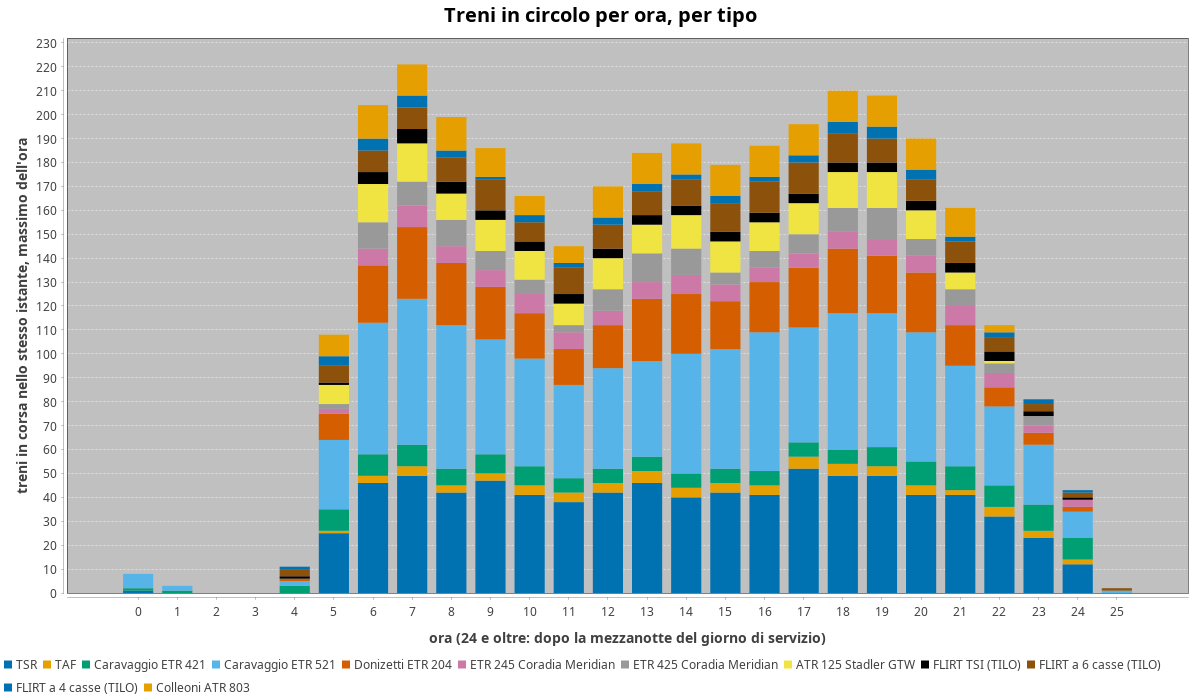
\includegraphics[width=\textwidth]{reale_treni_per_ora.png}
		\caption{Feriale.}
	\end{subfigure}
	\par\medskip
	\begin{subfigure}{\textwidth}
		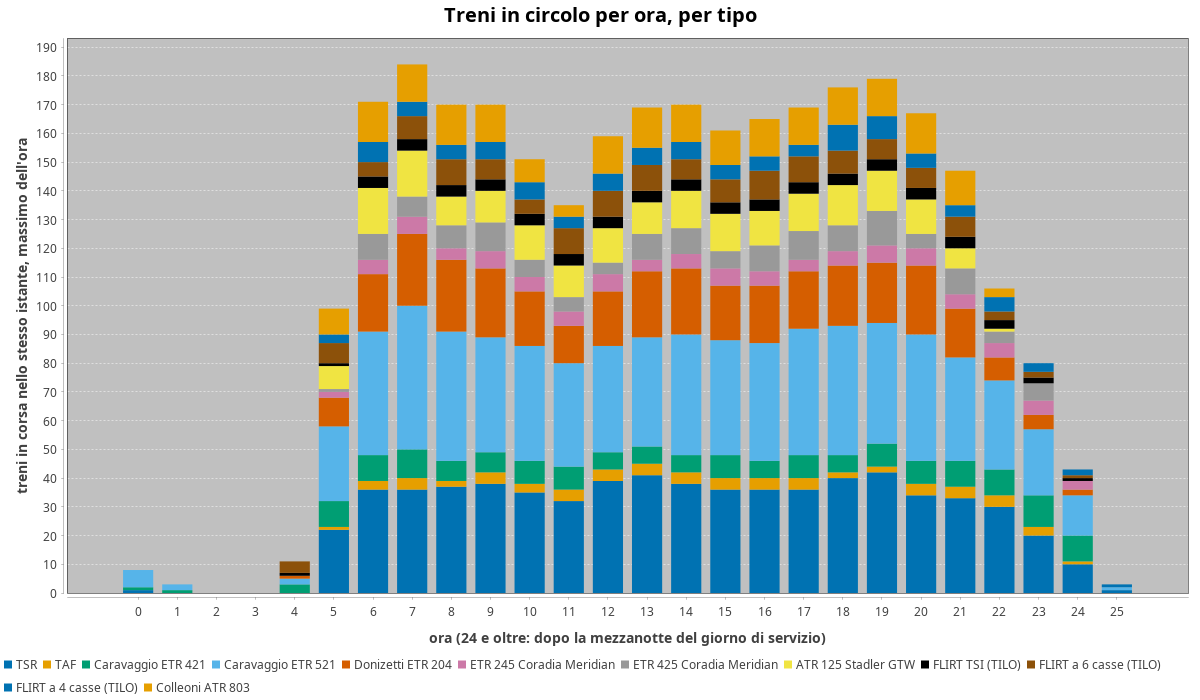
\includegraphics[width=\textwidth]{sabato_treni_per_ora.png}
		\caption{Sabato.}
	\end{subfigure}
	\caption{Orario reale: massimo di treni in corsa nello stesso istante, per ora e per tipo di treno, nel giorno feriale e il sabato.}
	\label{fig:reale-treni-giorni}
\end{figure}

\begin{figure}[H]
	\centering
	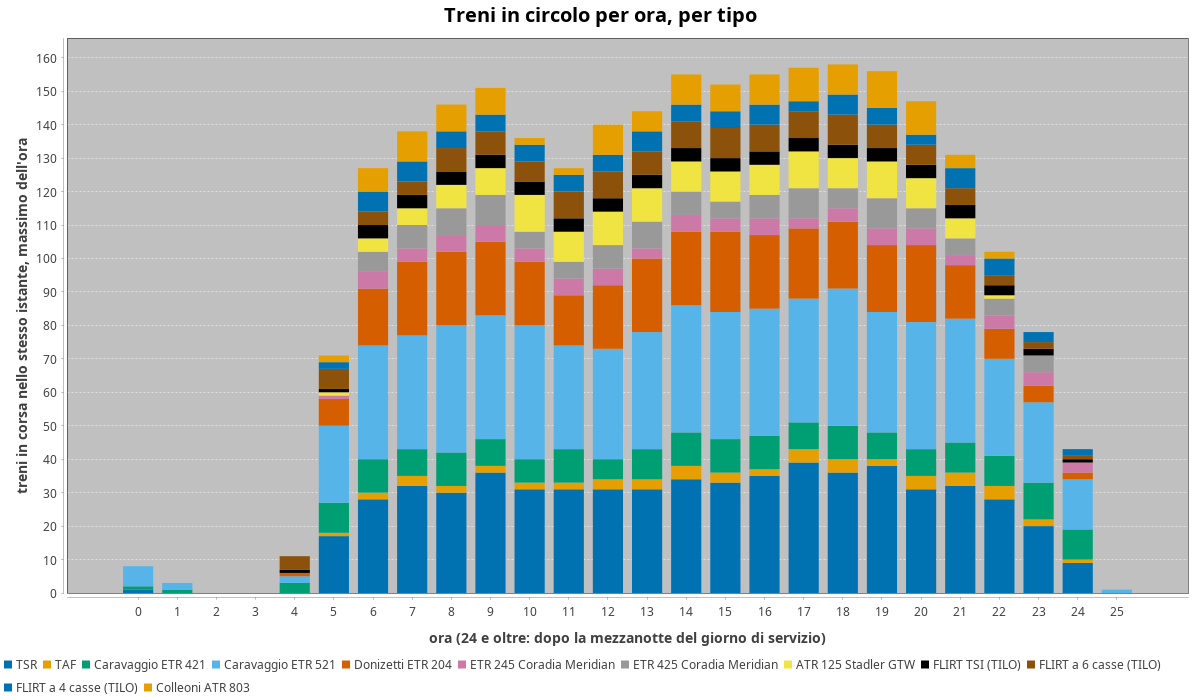
\includegraphics[width=\textwidth]{domenica_treni_per_ora.png}
	\caption{Orario reale: massimo di treni in corsa nello stesso istante, per ora e per tipo di treno, la domenica.}
	\label{fig:reale-treni-domenica}
\end{figure}

La puntualità è invece pressoché la stessa nei tre giorni, benché il carico della rete sia molto diverso. Lo mostra la \cref{fig:reale-ritardo-giorni}, che riporta il ritardo medio all'arrivo in fermata per ogni ora: nei tre giorni resta fra 0,6 e 1,1 minuti in tutte le ore di servizio, senza seguire le punte del numero di treni; il valore dell'ultima ora, dopo l'una di notte, riguarda poche corse.

\begin{figure}[H]
	\centering
	\begin{subfigure}{0.6\textwidth}
		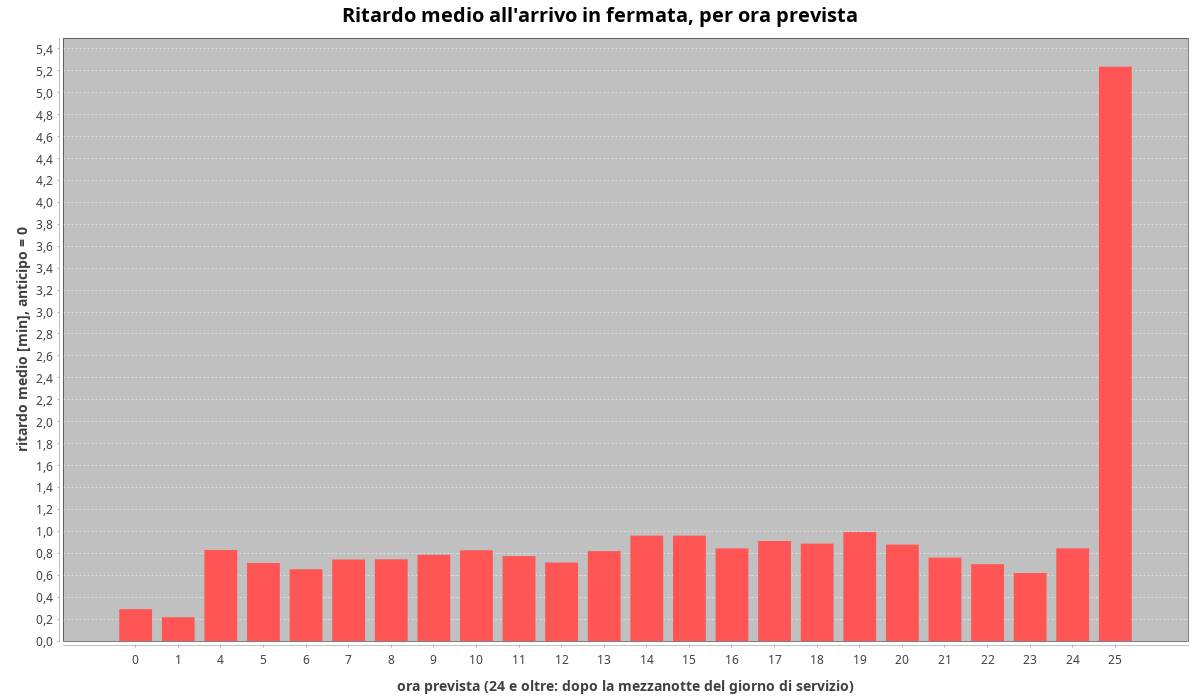
\includegraphics[width=\textwidth]{reale_ritardo_per_ora.png}
		\caption{Feriale.}
	\end{subfigure}
	\par\medskip
	\begin{subfigure}{0.6\textwidth}
		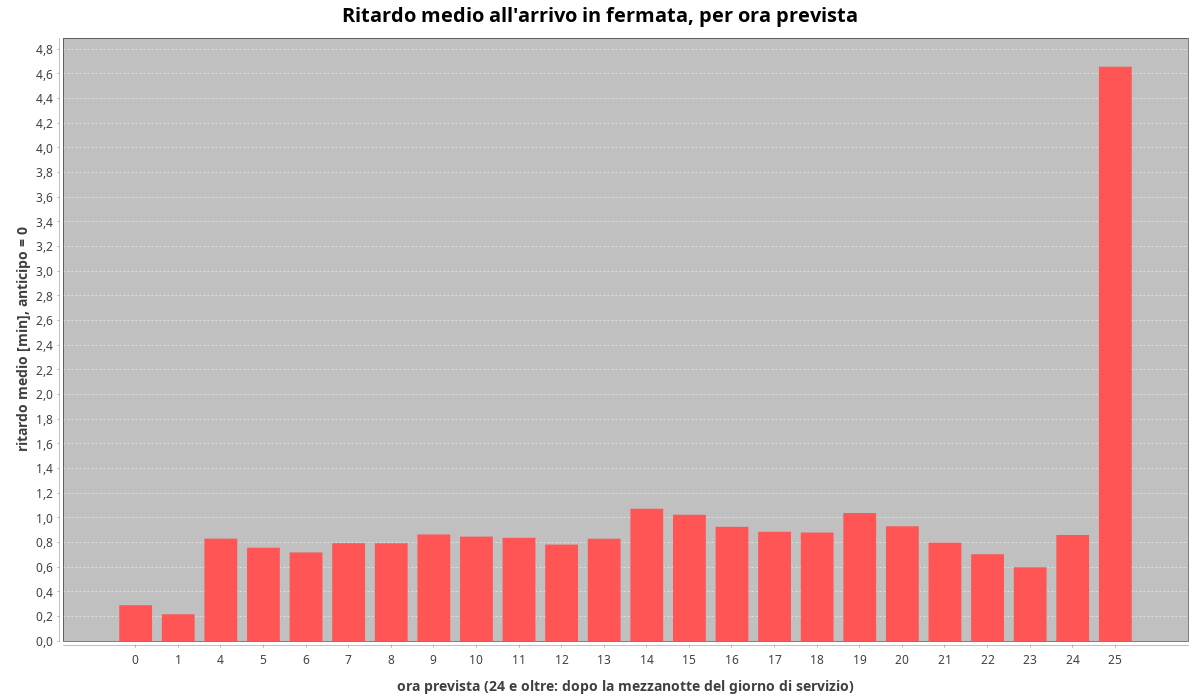
\includegraphics[width=\textwidth]{sabato_ritardo_per_ora.png}
		\caption{Sabato.}
	\end{subfigure}
	\par\medskip
	\begin{subfigure}{0.6\textwidth}
		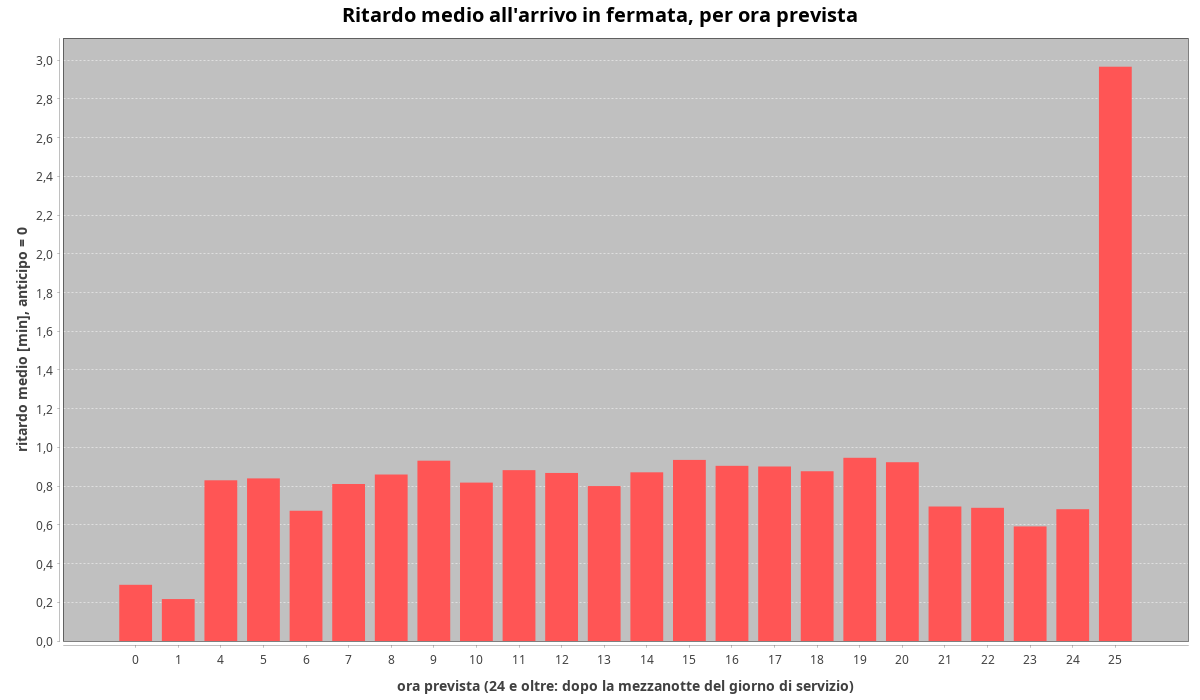
\includegraphics[width=\textwidth]{domenica_ritardo_per_ora.png}
		\caption{Domenica.}
	\end{subfigure}
	\caption{Orario reale: ritardo medio all'arrivo in fermata per ora prevista, nei tre tipi di giorno.}
	\label{fig:reale-ritardo-giorni}
\end{figure}

Nel modello i ritardi dell'orario reale non dipendono quindi dal carico complessivo, ma da punti precisi: le linee meno puntuali sono le stesse in tutti e tre i giorni, cioè R4, R5, RE11 e RE3. La R4 arriva puntuale a destinazione nel 3\% delle corse, la R5 fra il 33\% e il 52\%, la RE11 e la RE3 attorno al 50\%. Un ritardo che non cambia con il carico indica un punto in cui l'orario reale non è eseguibile sulla rete del modello così come è descritta, più che un effetto del traffico; è ripreso fra i limiti.

Due grandezze seguono invece il carico. La quota di energia di frenata riusata da altri treni scende dal 68\% del giorno feriale al 63\% della domenica: con meno treni in circolazione è meno probabile che un treno in trazione si trovi vicino a uno che frena. Il costo per treno-chilometro scende di poco, da \SI{10,49}{\euro} a \SI{10,17}{\euro}: la domenica i treni utilizzati diminuiscono più dei chilometri percorsi, e la voce del materiale rotabile pesa meno su ogni chilometro.

La \cref{fig:reale-ritardi} mostra come si distribuiscono gli scostamenti dall'orario nel giorno feriale. La maggior parte degli arrivi cade entro un minuto dall'orario previsto, e gli arrivi in anticipo sono più numerosi di quelli in ritardo: è l'effetto dei treni simulati più veloci dell'orario. La \cref{fig:reale-giornata} riporta le corse in corso nella giornata, con le due punte del servizio, e il diagramma spazio-tempo dei treni di una linea, la S1, in cui ogni tratto inclinato è una corsa e ogni tratto orizzontale una sosta. La \cref{fig:reale-treni} riporta i treni utilizzati nella giornata, divisi per tipo.

\begin{figure}[H]
	\centering
	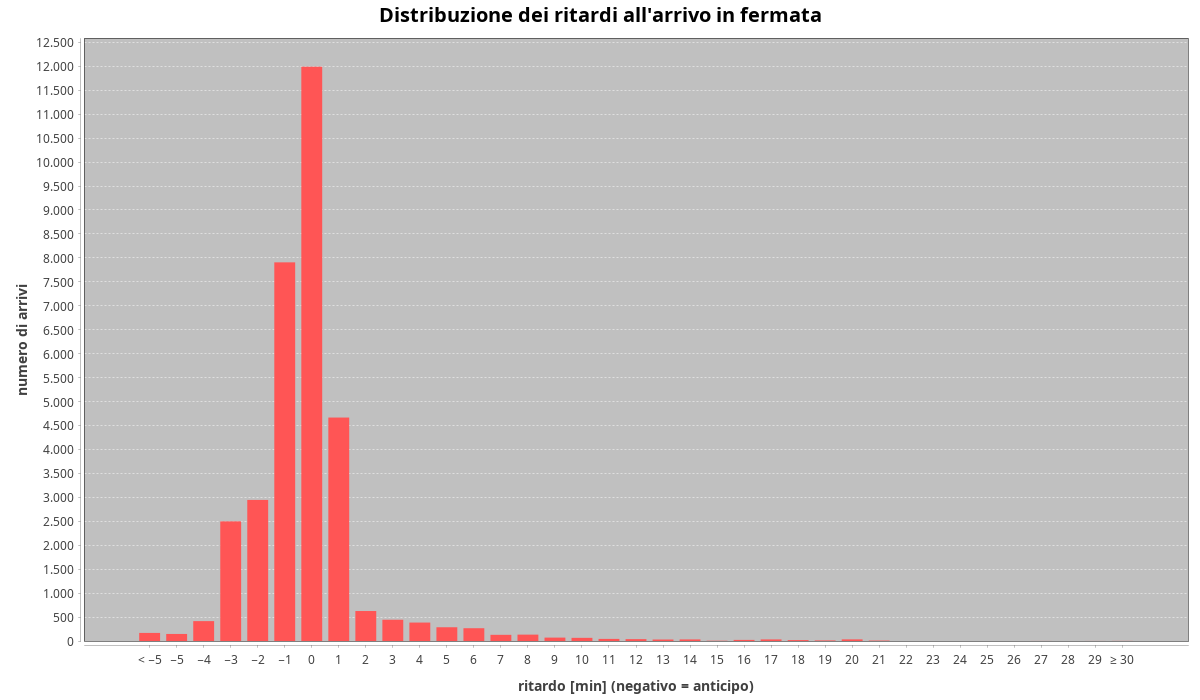
\includegraphics[width=0.7\textwidth]{reale_istogramma_ritardi.png}
	\caption{Giorno feriale reale: distribuzione degli scostamenti dall'orario all'arrivo in fermata. I valori negativi sono arrivi in anticipo.}
	\label{fig:reale-ritardi}
\end{figure}

\begin{figure}[H]
	\centering
	\begin{subfigure}{0.6\textwidth}
		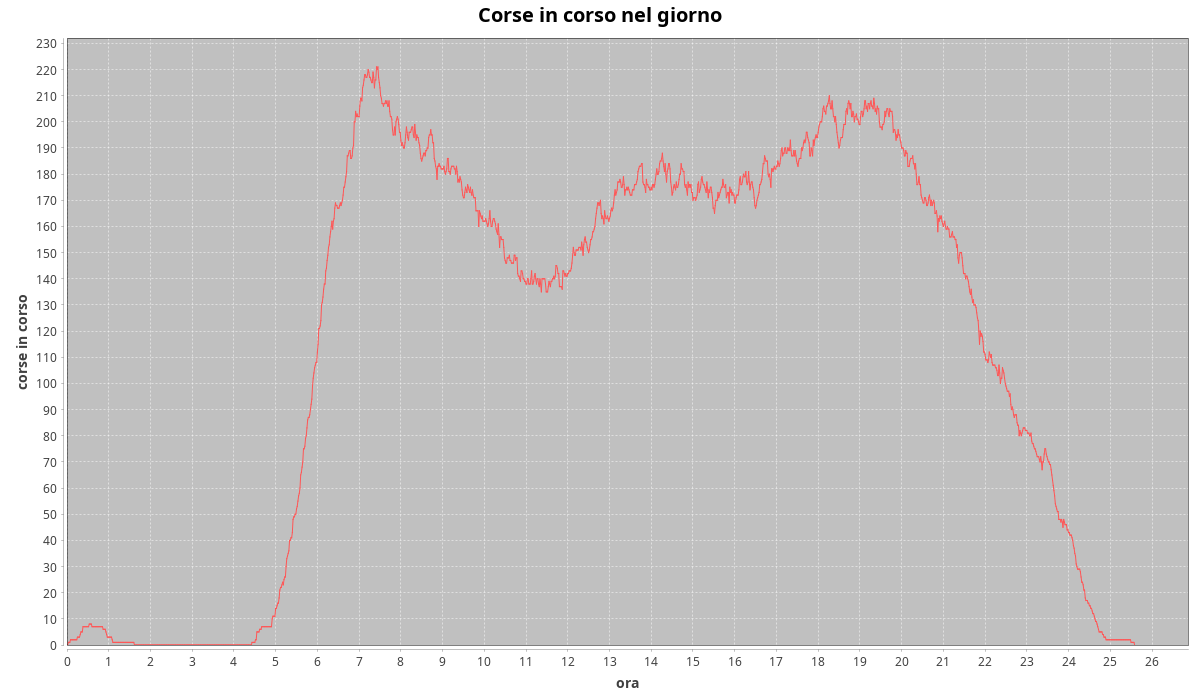
\includegraphics[width=\textwidth]{reale_corse_in_corso.png}
		\caption{Corse in corso nella giornata.}
	\end{subfigure}
	\par\medskip
	\begin{subfigure}{0.8\textwidth}
		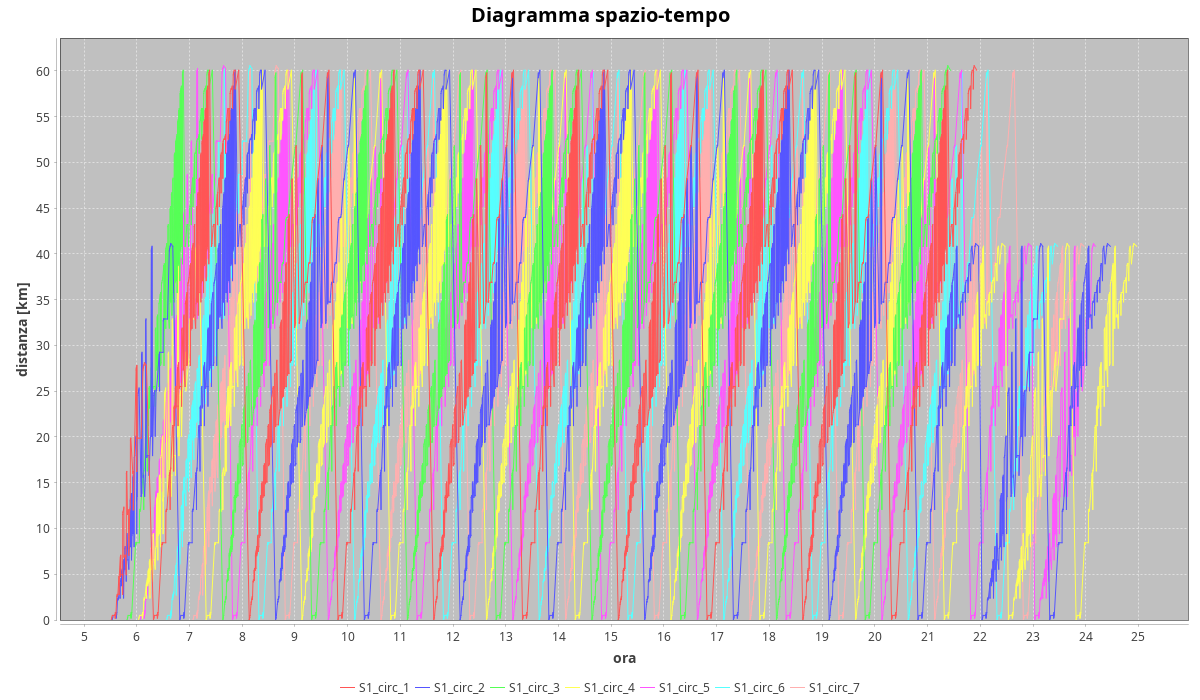
\includegraphics[width=\textwidth]{reale_spazio_tempo.png}
		\caption{Diagramma spazio-tempo dei treni della linea S1.}
	\end{subfigure}
	\caption{Giorno feriale reale: andamento del servizio nella giornata.}
	\label{fig:reale-giornata}
\end{figure}

\begin{figure}[H]
	\centering
	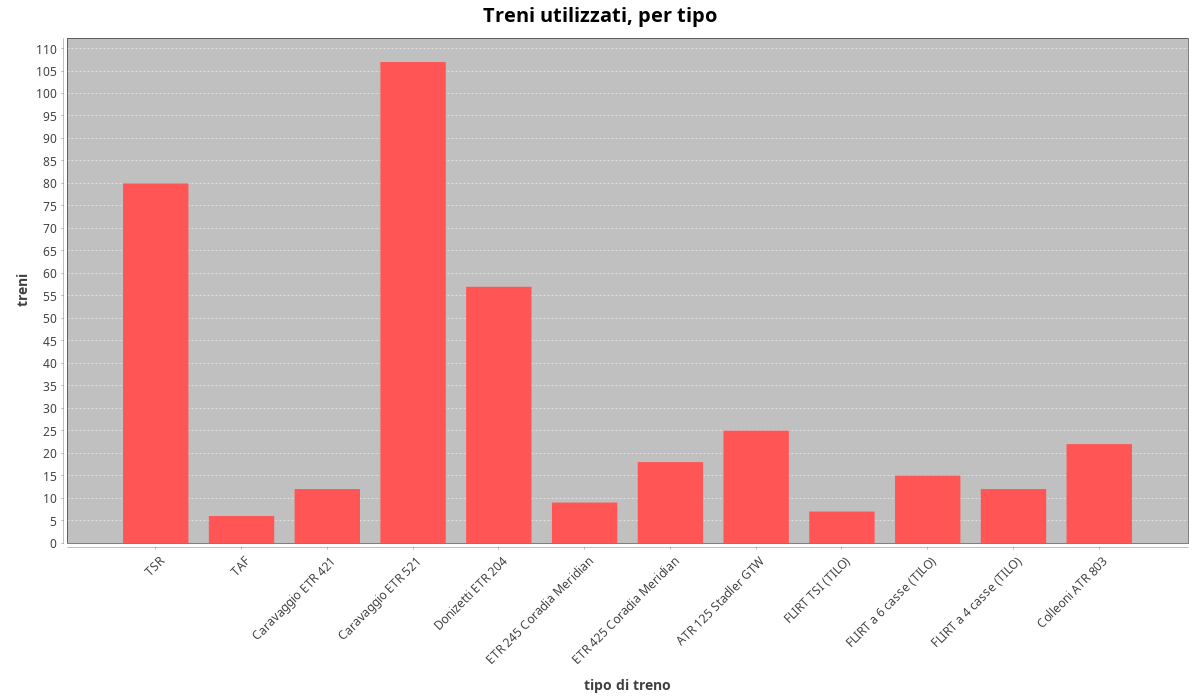
\includegraphics[width=0.7\textwidth]{reale_flotta.png}
	\caption{Giorno feriale reale: treni utilizzati, per tipo.}
	\label{fig:reale-treni}
\end{figure}

\subsection{Passante ad alta frequenza}
La \cref{tab:risultati-passante} confronta il giorno feriale reale con lo scenario del Passante ai due obiettivi. Con l'obiettivo di 15 minuti le corse aggiunte sono 47, con quello di 10 minuti 189.

\begin{table}[H]
	\centering
	\caption{Giorno feriale: orario reale e Passante ad alta frequenza.}
	\label{tab:risultati-passante}
	\begin{tabularx}{\textwidth}{Xrrr}
		\toprule
		Indicatore & Reale & Passante a 15 minuti & Passante a 10 minuti \\
		\midrule
		Corse & 2349 & 2396 & 2538 \\
		Regolarità & 100\% & 100\% & 100\% \\
		Puntualità a destinazione & 94,1\% & 93,9\% & 91,6\% \\
		Puntualità su tutte le fermate & 96,7\% & 96,6\% & 94,2\% \\
		Ritardo medio & \SI{47}{\second} & \SI{49}{\second} & \SI{87}{\second} \\
		95\textsuperscript{o} percentile del ritardo & \SI{210}{\second} & \SI{220}{\second} & \SI{353}{\second} \\
		Treni utilizzati & 343 & 353 & 376 \\
		Massimo di treni in corsa insieme & 207 & 213 & 227 \\
		Costo simulato & \SI{1509171}{\euro} & \SI{1535044}{\euro} & \SI{1609502}{\euro} \\
		\bottomrule
	\end{tabularx}
\end{table}

In entrambi i casi tutte le corse vengono completate: la rete regge l'orario aggiunto. Con l'obiettivo di 15 minuti gli indicatori sono quasi invariati, perché le 47 corse aggiunte riguardano la S9 e i tratti di Cormano e di Monza, mentre nel tunnel, dove l'attesa massima è già di 15 minuti, non viene aggiunto nulla. Con quello di 10 minuti la puntualità a destinazione scende di due punti e mezzo e il ritardo medio quasi raddoppia. La \cref{fig:passante-ritardo} mostra che il ritardo in più si concentra nelle ore in cui lo scenario aggiunge corse: nel giorno reale il ritardo medio è quasi piatto, mentre con lo scenario compaiono due picchi, fra le 9 e le 10 e fra le 18 e le 20, in cui supera i due minuti. I picchi seguono di un'ora o due le punte del servizio: il ritardo si accumula durante la punta e si smaltisce dopo. La distribuzione degli scostamenti è nella \cref{fig:passante-istogramma}, e l'andamento della giornata nella \cref{fig:passante-giornata}.

\begin{figure}[H]
	\centering
	\begin{subfigure}{0.6\textwidth}
		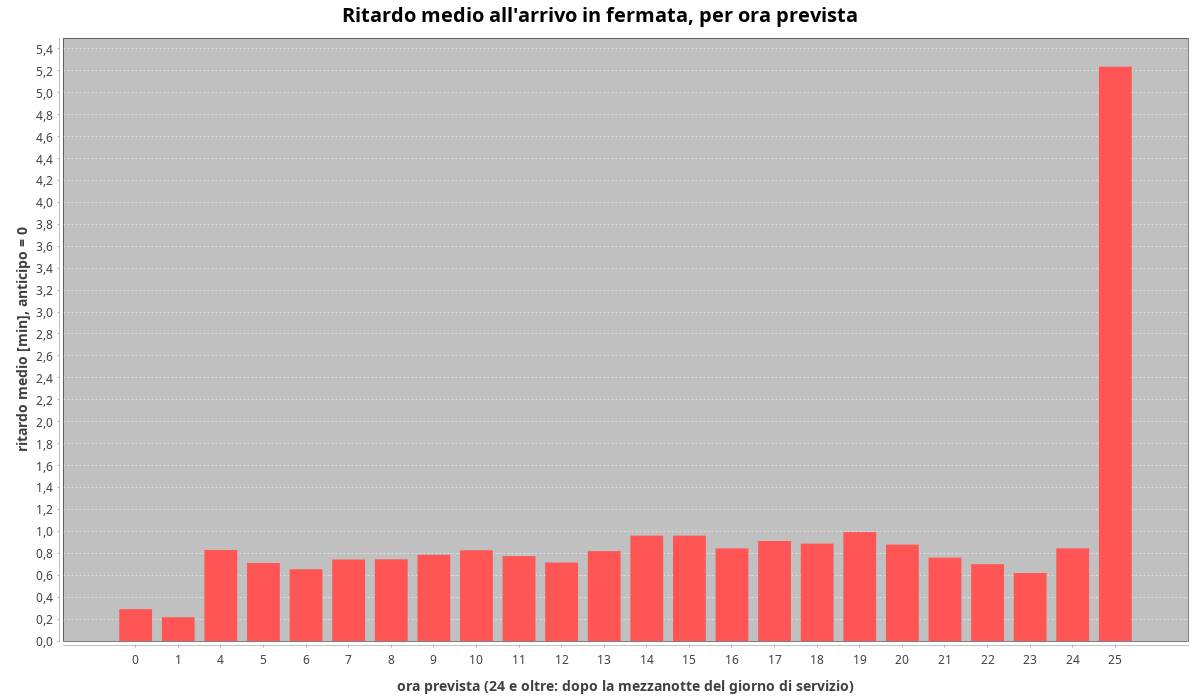
\includegraphics[width=\textwidth]{reale_ritardo_per_ora.png}
		\caption{Orario reale.}
	\end{subfigure}
	\par\medskip
	\begin{subfigure}{0.6\textwidth}
		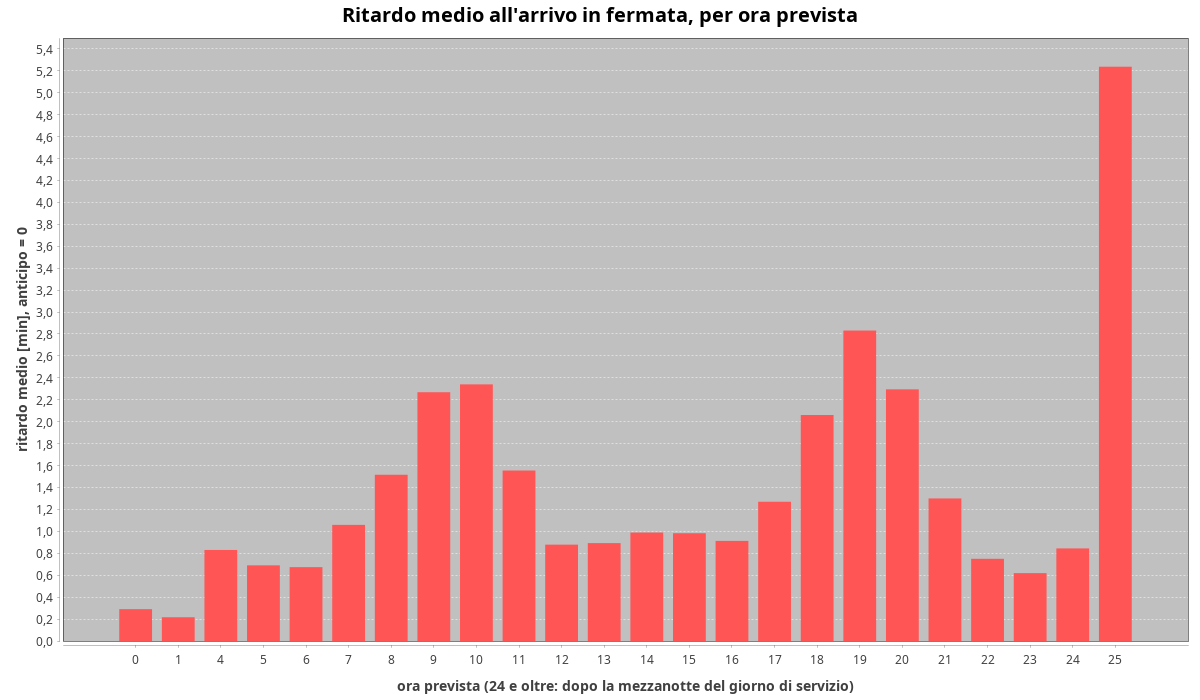
\includegraphics[width=\textwidth]{passante10_ritardo_per_ora.png}
		\caption{Passante a 10 minuti.}
	\end{subfigure}
	\caption{Giorno feriale: ritardo medio all'arrivo in fermata per ora prevista.}
	\label{fig:passante-ritardo}
\end{figure}

\begin{figure}[H]
	\centering
	\begin{subfigure}{0.6\textwidth}
		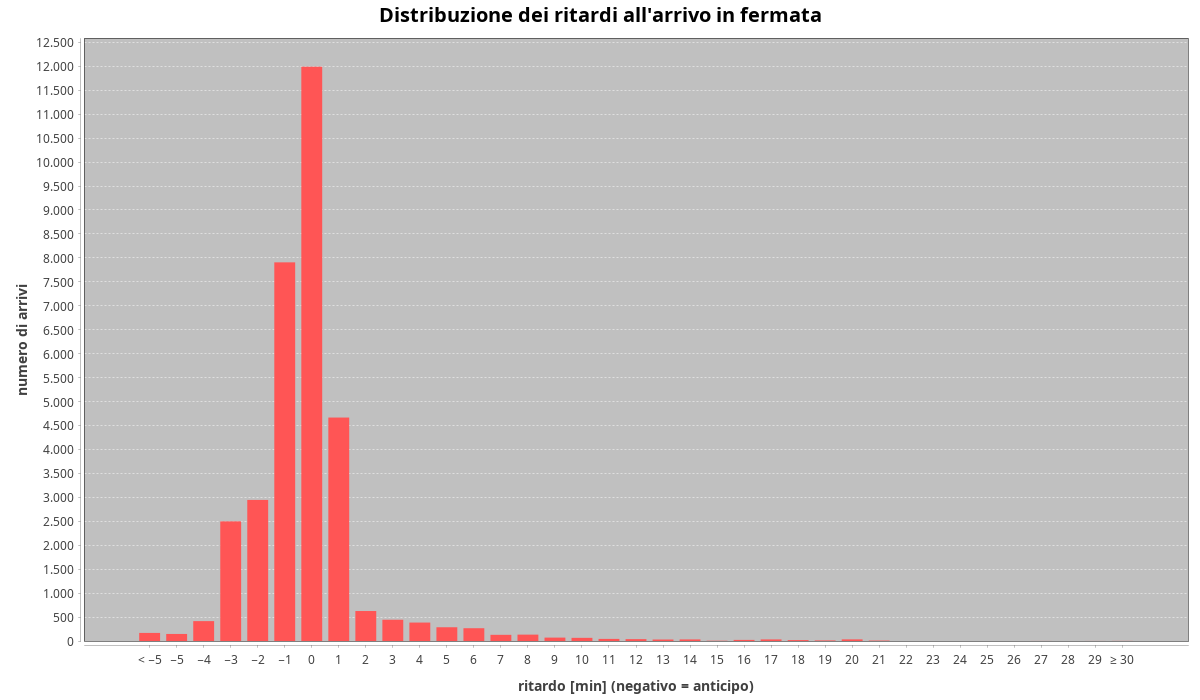
\includegraphics[width=\textwidth]{reale_istogramma_ritardi.png}
		\caption{Orario reale.}
	\end{subfigure}
	\par\medskip
	\begin{subfigure}{0.6\textwidth}
		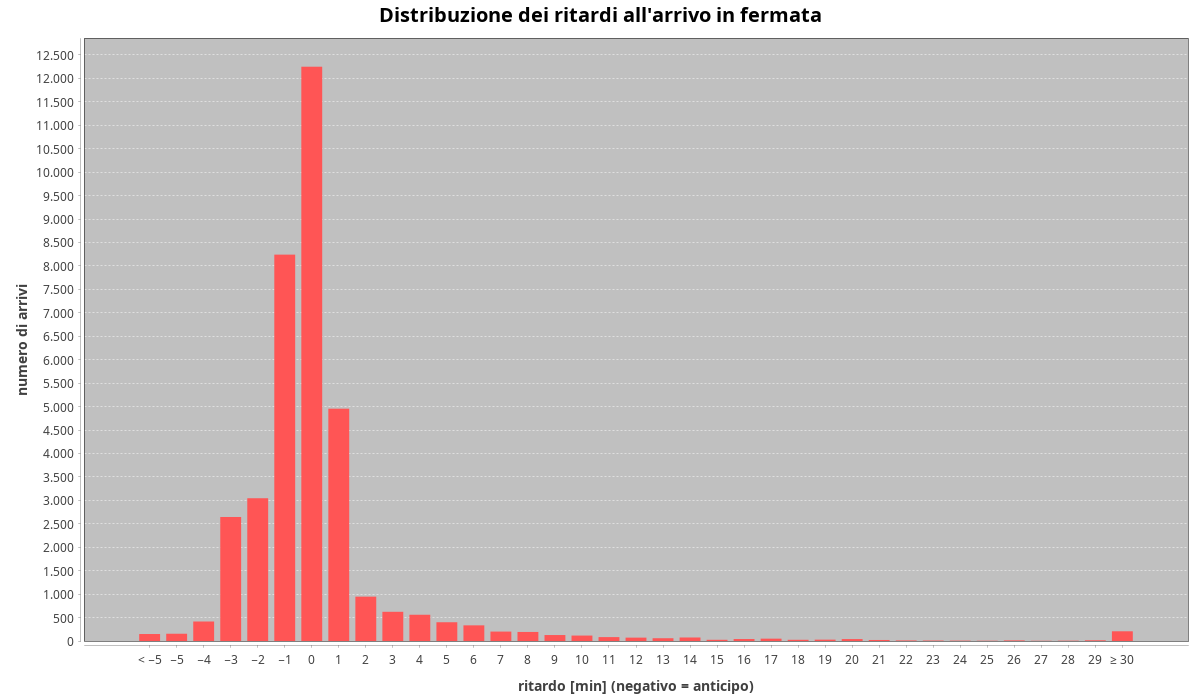
\includegraphics[width=\textwidth]{passante10_istogramma_ritardi.png}
		\caption{Passante a 10 minuti.}
	\end{subfigure}
	\caption{Giorno feriale: distribuzione degli scostamenti all'arrivo in fermata.}
	\label{fig:passante-istogramma}
\end{figure}

\begin{figure}[H]
	\centering
	\begin{subfigure}{0.6\textwidth}
		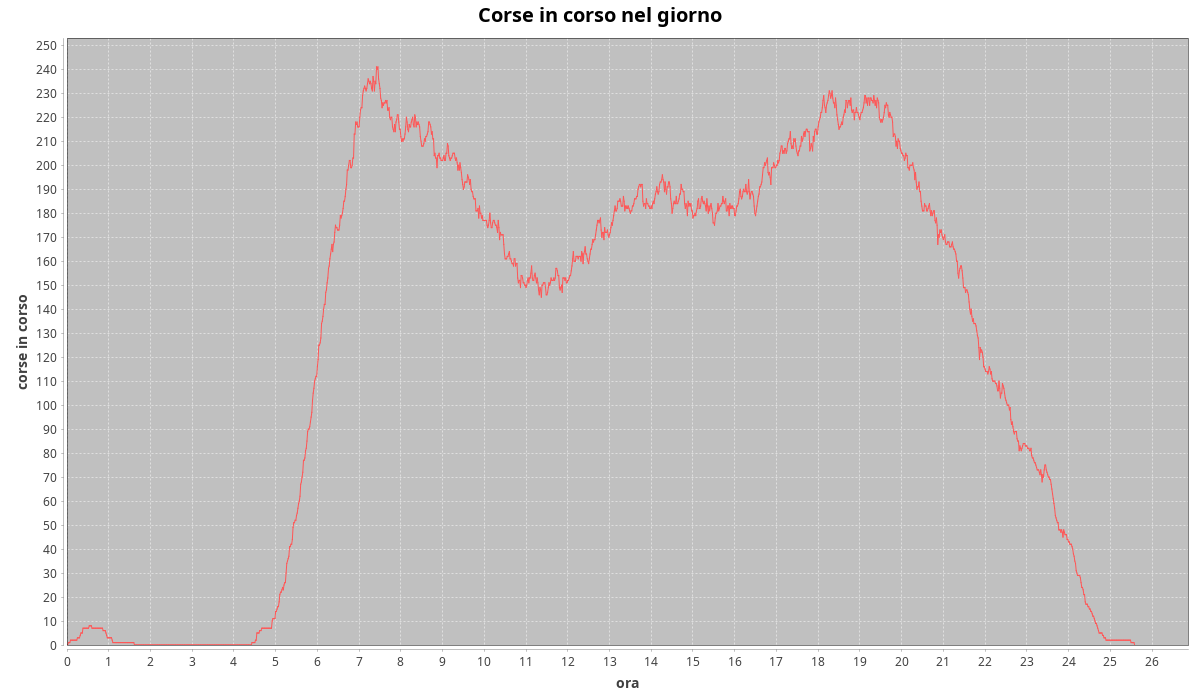
\includegraphics[width=\textwidth]{passante10_corse_in_corso.png}
		\caption{Corse in corso nella giornata.}
	\end{subfigure}
	\par\medskip
	\begin{subfigure}{0.8\textwidth}
		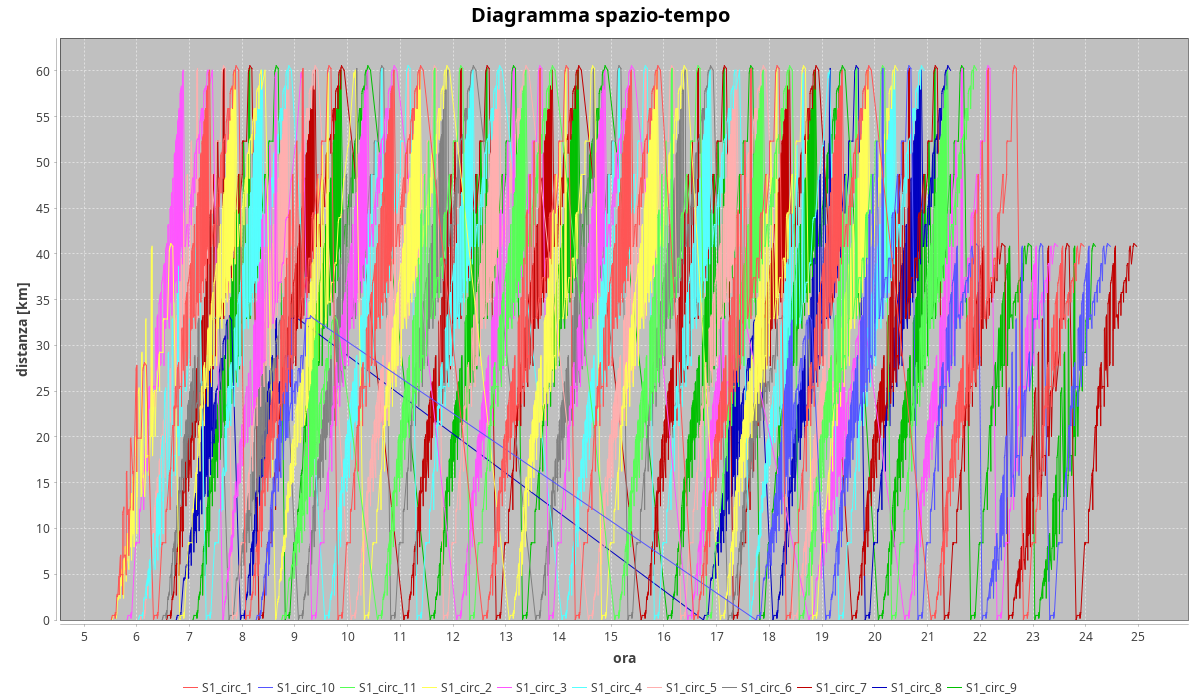
\includegraphics[width=\textwidth]{passante10_spazio_tempo.png}
		\caption{Diagramma spazio-tempo dei treni della linea S1.}
	\end{subfigure}
	\caption{Passante a 10 minuti, giorno feriale: andamento del servizio nella giornata.}
	\label{fig:passante-giornata}
\end{figure}

Il peggioramento non è distribuito in modo uniforme, come mostra la \cref{tab:risultati-linee}. Riguarda quasi soltanto la linea S9, le cui corse passano da 73 a 155: la puntualità a destinazione scende dal 100\% al 66,5\% e il ritardo medio sale da 29 a 405 secondi, con un 95\textsuperscript{o} percentile di 35 minuti. Le altre linee potenziate restano puntuali, comprese quelle che attraversano il tunnel. Due linee non potenziate peggiorano perché condividono i binari con una linea potenziata: la R16 con la S4 verso Cadorna, e la R31 con la S9.

\begin{table}[H]
	\centering
	\caption{Giorno feriale, obiettivo di 10 minuti: linee potenziate e linee che ne risentono.}
	\label{tab:risultati-linee}
	\begin{tabularx}{\textwidth}{Xrrrrrr}
		\toprule
		 & \multicolumn{2}{c}{Corse} & \multicolumn{2}{c}{Puntualità a destinazione} & \multicolumn{2}{c}{Ritardo medio (s)} \\
		Linea & reale & scenario & reale & scenario & reale & scenario \\
		\midrule
		S1 & 74 & 86 & 100\% & 100\% & 16 & 16 \\
		S2 & 62 & 86 & 100\% & 94,2\% & 11 & 49 \\
		S4 & 73 & 131 & 100\% & 96,2\% & 28 & 50 \\
		S9 & 73 & 155 & 100\% & 66,5\% & 29 & 405 \\
		S12 & 60 & 66 & 100\% & 100\% & 6 & 6 \\
		S13 & 74 & 79 & 100\% & 100\% & 12 & 12 \\
		\midrule
		R16 & 56 & 56 & 87,5\% & 75,0\% & 61 & 117 \\
		R31 & 48 & 48 & 100\% & 100\% & 16 & 47 \\
		\bottomrule
	\end{tabularx}
\end{table}

La S9 è l'unica delle linee potenziate ad avere una tratta a binario unico, fra Seregno e Cesano Maderno, e a quella frequenza i treni dei due versi non riescono più a incrociarsi senza attendersi. Con l'obiettivo di 15 minuti la stessa linea, con 97 corse, resta al 100\% di puntualità, e lo stesso accade il sabato con 129 corse e la domenica con 117: la soglia si trova quindi fra 129 e 155 corse al giorno. Il risultato va letto in due modi. Mostra che il limite di una linea non è nel suo tratto più carico ma nel suo punto più stretto, e che una linea può saturarsi mentre il resto della rete, tunnel compreso, regge. E mostra la non linearità del sistema: passando da 129 a 155 corse il ritardo medio si moltiplica per dieci.

\subsubsection{Lo scenario nei tre tipi di giorno}
La \cref{tab:risultati-passante-giorni} confronta lo scenario con obiettivo di 10 minuti nei tre tipi di giorno. Con l'obiettivo di 15 minuti il confronto non è possibile, perché il sabato e la domenica quello scenario non aggiunge corse.

\begin{table}[H]
	\centering
	\caption{Scenario del Passante con obiettivo di 10 minuti nei tre tipi di giorno. Dove compaiono due valori, il primo è dell'orario reale dello stesso giorno.}
	\label{tab:risultati-passante-giorni}
	\begin{tabularx}{\textwidth}{Xrrr}
		\toprule
		Indicatore & Feriale & Sabato & Domenica \\
		\midrule
		Corse aggiunte & 189 & 169 & 133 \\
		\quad Bovisa--Passante & 47 & 56 & 44 \\
		\quad Saronno--Albairate (S9) & 82 & 56 & 44 \\
		\quad Cormano--Cadorna & 58 & 57 & 45 \\
		\quad Monza--Garibaldi & 2 & 0 & 0 \\
		\midrule
		Regolarità & 100\% & 100\% & 100\% \\
		Puntualità a destinazione & 94,1 $\rightarrow$ 91,6\% & 93,8 $\rightarrow$ 93,5\% & 94,5 $\rightarrow$ 94,3\% \\
		Ritardo medio (s) & 47 $\rightarrow$ 87 & 50 $\rightarrow$ 52 & 49 $\rightarrow$ 51 \\
		Corse della S9 & 73 $\rightarrow$ 155 & 73 $\rightarrow$ 129 & 73 $\rightarrow$ 117 \\
		Puntualità a destinazione della S9 & 100 $\rightarrow$ 66,5\% & 100 $\rightarrow$ 100\% & 100 $\rightarrow$ 100\% \\
		\midrule
		Treni in più & 33 & 18 & 18 \\
		Costo simulato in più & 6,6\% & 5,4\% & 5,1\% \\
		\bottomrule
	\end{tabularx}
\end{table}

Il sabato e la domenica lo scenario non peggiora la puntualità, mentre nel giorno feriale la riduce di due punti e mezzo. La differenza non dipende dal carico della rete nel fine settimana, ma dalla regola dello scenario: fuori dalle ore di punta dei giorni feriali l'obiettivo di 10 minuti diventa di 15. La S9 riceve quindi 82 corse nel giorno feriale e 56 il sabato, e resta sotto la soglia oltre la quale il suo tratto a binario unico cede. Il confronto conferma dunque, da un'altra direzione, che il peggioramento del giorno feriale è dovuto a quella sola linea.

I treni in più sono 18 il sabato e la domenica contro i 33 del giorno feriale, e in tutti e tre i casi sono dei tipi che servono le linee suburbane. Il costo cresce in proporzione simile nei tre giorni, fra il 5\% e il 7\%.

\subsection{Treni necessari e flotta disponibile}
Uno scenario che aggiunge corse richiede treni in più, e la domanda è se l'operatore ne dispone. La \cref{tab:risultati-flotta} confronta, per tipo, i treni utilizzati nelle tre simulazioni del giorno feriale con quelli disponibili.

\begin{table}[H]
	\centering
	\caption{Treni utilizzati in un giorno feriale e treni disponibili, per tipo.}
	\label{tab:risultati-flotta}
	\begin{tabularx}{\textwidth}{Xrrrr}
		\toprule
		Tipo & Disponibili & Reale & Passante a 15 min & Passante a 10 min \\
		\midrule
		Caravaggio & 136 & 119 & 123 & 127 \\
		TSR & circa 104 & 80 & 85 & 101 \\
		Donizetti & 61 & 57 & 57 & 57 \\
		ETR 425 e 526 & 54 & 18 & 18 & 18 \\
		TAF & 34 & 6 & 6 & 9 \\
		Colleoni & 30 & 22 & 22 & 22 \\
		ETR 245 & 14 & 9 & 10 & 10 \\
		ATR 125 & 20 & 25 & 25 & 25 \\
		Flirt TILO & 9 & 7 & 7 & 7 \\
		\midrule
		Totale & & 343 & 353 & 376 \\
		\bottomrule
	\end{tabularx}
\end{table}

\begin{figure}[H]
	\centering
	\begin{subfigure}{\textwidth}
		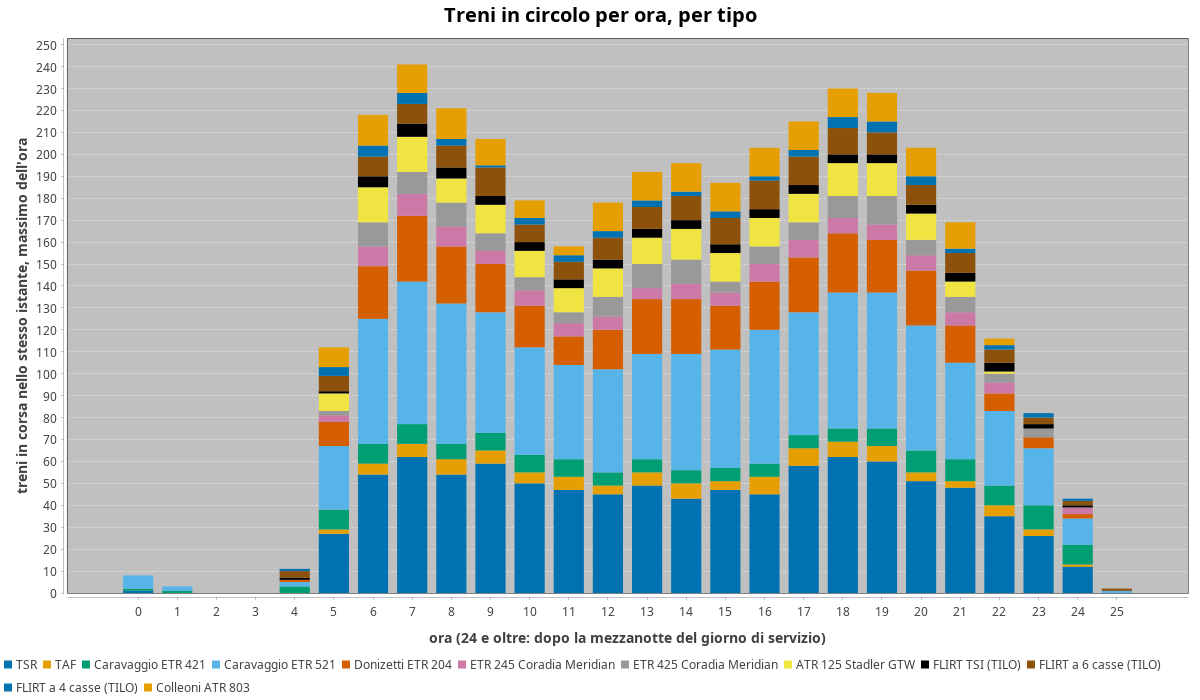
\includegraphics[width=\textwidth]{passante10_treni_per_ora.png}
		\caption{Massimo di treni in corsa insieme, per ora e per tipo.}
	\end{subfigure}
	\par\medskip
	\begin{subfigure}{0.7\textwidth}
		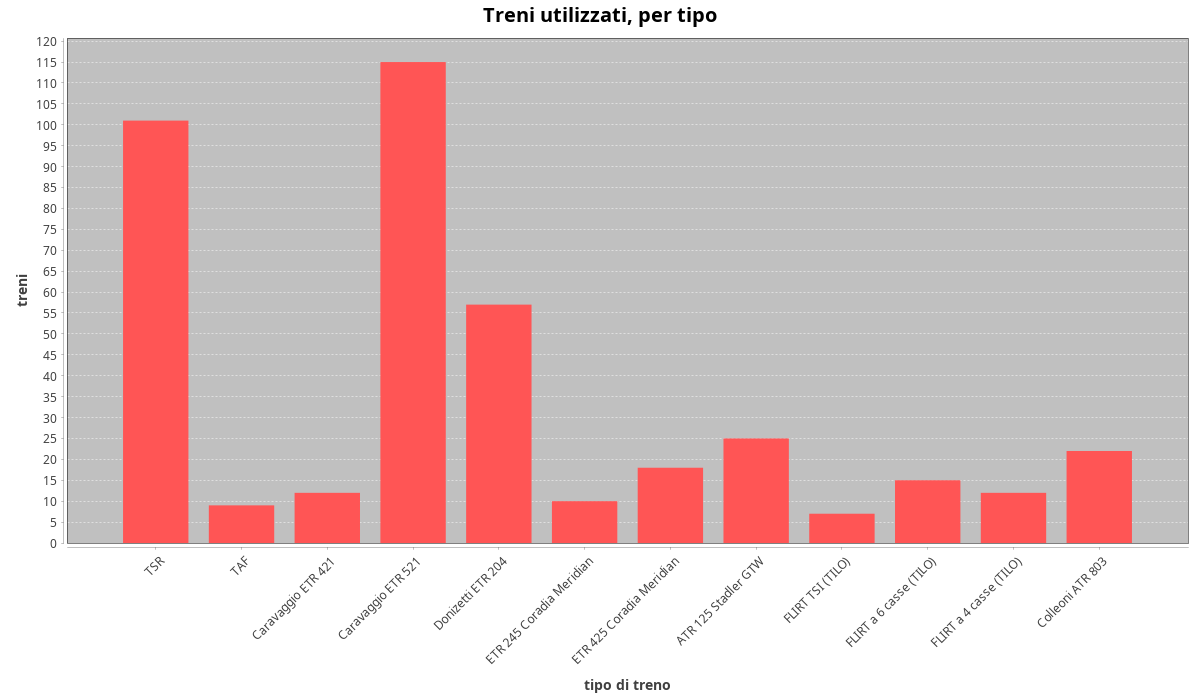
\includegraphics[width=\textwidth]{passante10_flotta.png}
		\caption{Treni utilizzati, per tipo.}
	\end{subfigure}
	\caption{Passante a 10 minuti, giorno feriale: treni in servizio. I grafici corrispondenti dell'orario reale sono nelle \cref{fig:reale-treni-giorni,fig:reale-treni}.}
	\label{fig:passante-treni}
\end{figure}

Lo scenario a 15 minuti richiede 10 treni in più, quello a 10 minuti 33; il sabato e la domenica, con l'obiettivo di 10 minuti, 18 in entrambi i casi. In tutte le simulazioni ogni tipo resta entro la disponibilità, con una sola eccezione, gli ATR 125, che nel modello sono 25 contro 20: nella realtà la differenza è coperta da altri tipi di automotrice diesel, che il modello non contiene. Sulla carta, dunque, lo scenario del Passante non richiede l'acquisto di treni.

Il margine è però ridotto. Con l'obiettivo di 10 minuti i TSR utilizzati sono 101 su circa 104, e il conto non comprende i treni di riserva né quelli in manutenzione, che in una flotta reale sono una quota non trascurabile. Se i 33 treni in più dovessero essere acquistati, al prezzo delle ultime commesse dell'operatore, fra 8,5 e 10 milioni di euro a treno, l'investimento sarebbe dell'ordine di 280--330 milioni: una stima di larga massima, da leggere come ordine di grandezza. \\
Valgono le cautele già indicate. I treni contati sono quelli dei giri treno del modello, e la ripartizione per tipo deriva dalle quote per linea, che sono una stima. Il dato solido è la differenza fra scenario e giorno reale.

\subsection{Potenziamento per linea}
Il secondo scenario è stato usato per cercare il limite, con cinque simulazioni a obiettivi via via meno ambiziosi, riassunte nella \cref{tab:risultati-potenziamento}. In tutti i casi i percorsi non indicati sono portati a 30 minuti.

\begin{table}[H]
	\centering
	\caption{Potenziamento per linea: le cinque simulazioni. I casi da A a D sono del giorno feriale, il caso E del sabato.}
	\label{tab:risultati-potenziamento}
	\begin{tabularx}{\textwidth}{lXrrrr}
		\toprule
		Caso & Linee sotto i 30 minuti & Corse & Regolarità & Treni non arrivati & Avvisi nel tunnel \\
		\midrule
		A & S1 e S3 a 10; le altre suburbane e gran parte dei RegioExpress a 15 & 4809 & 40,1\% & 474 su 636 & 420 \\
		B & S1, S3, S4, S5, S9 e otto RegioExpress a 15 & 3992 & 73,5\% & 319 su 564 & 125 \\
		C & S1, S5, R17 e cinque RegioExpress a 15 & 3606 & 65,8\% & 312 su 523 & 125 \\
		D & nessuna: tutti i percorsi a 30 & 3163 & 94,3\% & 72 su 471 & 6 \\
		E & S1, S3, S4, S8, S11, R17 e tre RegioExpress a 15 & 3377 & 93,8\% & 77 su 445 & 9 \\
		\bottomrule
	\end{tabularx}
\end{table}

Nessuna delle cinque simulazioni completa tutte le corse. Il caso A, che raddoppia il servizio reale, è il più istruttivo. Dalla registrazione si vede dove comincia: dalle 7:36 i binari terminali di Milano Rogoredo sono tutti occupati, i treni in arrivo si fermano alla stazione precedente e quelli in partenza non riescono a uscire; in mezz'ora la coda risale il Passante e poi si estende alla rete. La causa è nella \cref{tab:risultati-tunnel}: lo scenario chiede al tunnel più del doppio dei treni di oggi. Con un intervallo di 180 secondi il tunnel ammette al più 20 treni all'ora per verso, e lo scenario ne chiede fino a 27. Nel potenziamento per linea ogni percorso è aumentato per conto proprio, e le sei linee del Passante sommano le loro corse nello stesso tunnel; lo scenario stesso lo segnala prima della simulazione, con 420 passaggi sotto l'intervallo di riferimento.

\begin{table}[H]
	\centering
	\caption{Treni all'ora nel tunnel del Passante, per verso, nell'ora di punta del mattino.}
	\label{tab:risultati-tunnel}
	\begin{tabularx}{\textwidth}{Xrrr}
		\toprule
		 & Reale & Passante a 10 minuti & Potenziamento, caso A \\
		\midrule
		Verso Rogoredo & 12 & 16 & 24--25 \\
		Verso Bovisa & 12 & 16 & 26--27 \\
		Capacità a 180 secondi & 20 & 20 & 20 \\
		\bottomrule
	\end{tabularx}
\end{table}

La \cref{fig:potenziamento-corse} mostra l'effetto sull'intera giornata. Nel giorno reale le corse in corso seguono le due punte del servizio. Nel caso A salgono fino alle 7:30, poi scendono a un valore quasi costante per il resto del giorno: sono i treni fermi che non concludono la corsa, mentre le corse successive non partono. La \cref{fig:potenziamento-stallo} mostra la rete alla fine della giornata, con i treni fermi lungo le linee che convergono su Milano.

\begin{figure}[H]
	\centering
	\begin{subfigure}{0.6\textwidth}
		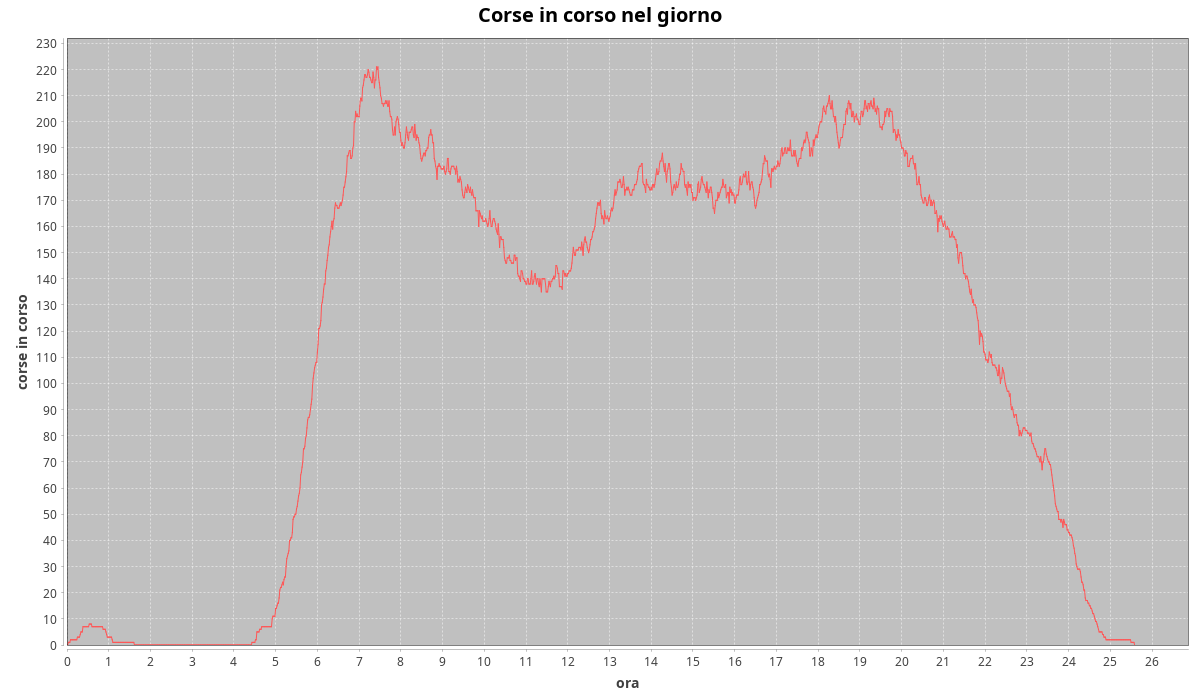
\includegraphics[width=\textwidth]{reale_corse_in_corso.png}
		\caption{Orario reale.}
	\end{subfigure}
	\par\medskip
	\begin{subfigure}{0.6\textwidth}
		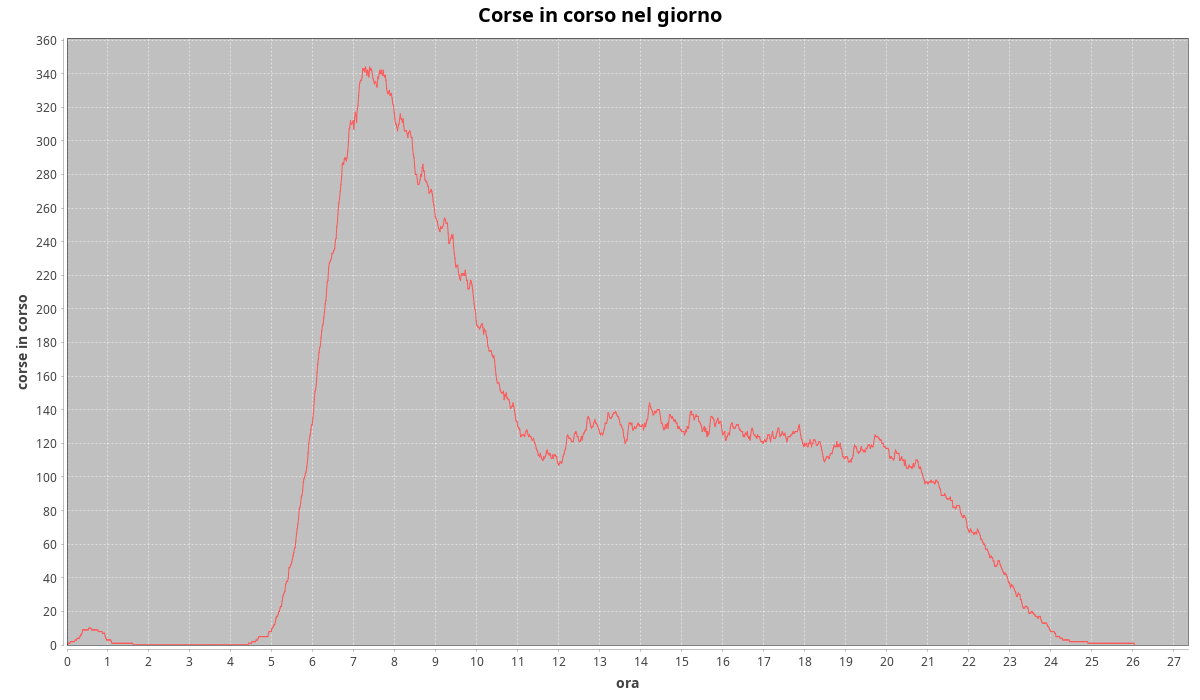
\includegraphics[width=\textwidth]{potenziamentoA_corse_in_corso.png}
		\caption{Potenziamento, caso A.}
	\end{subfigure}
	\caption{Giorno feriale: corse in corso nella giornata. Le due scale verticali sono diverse.}
	\label{fig:potenziamento-corse}
\end{figure}

\begin{figure}[H]
	\centering
	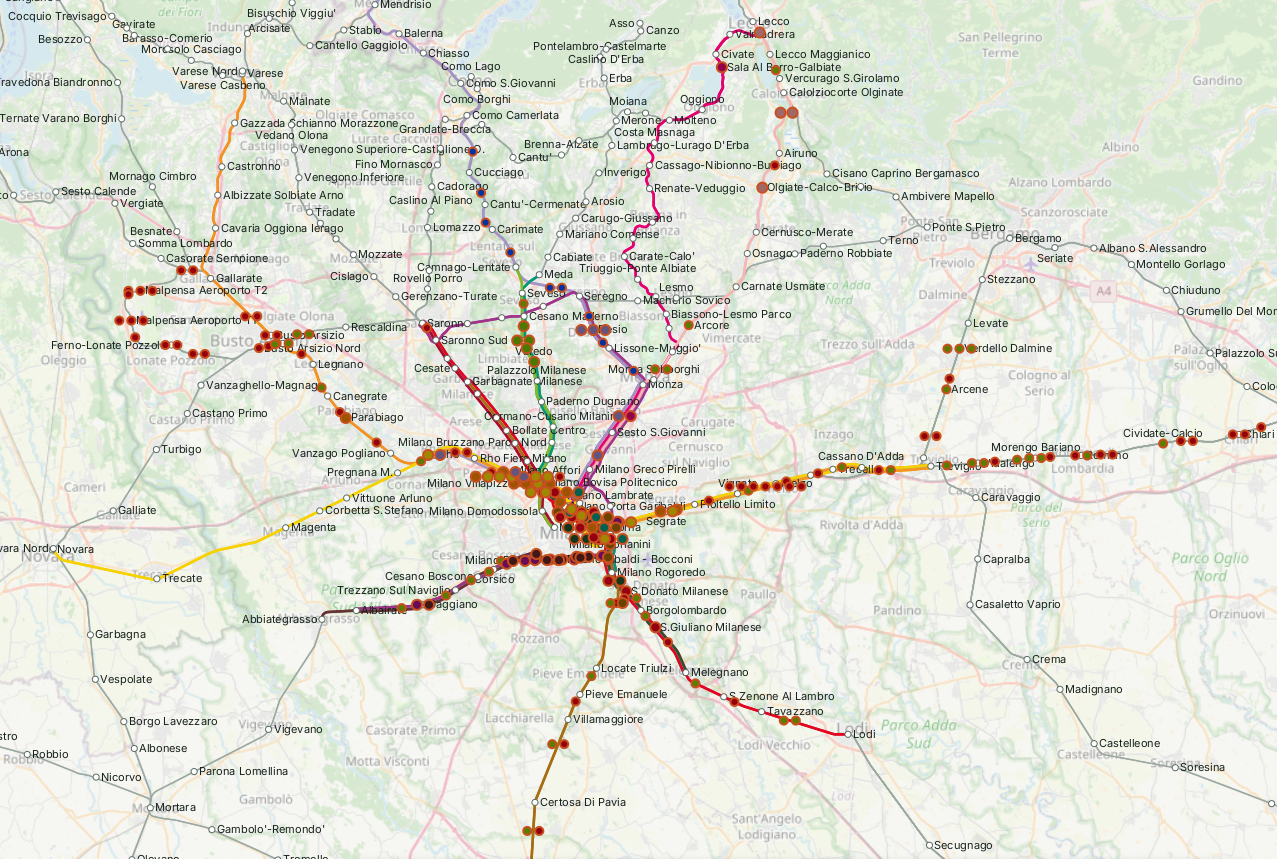
\includegraphics[width=0.8\textwidth]{simulazione_potenziamento_a_finegiornata_trenibloccati.png}
	\caption{Potenziamento, caso A: treni fermi sulla rete a fine giornata.}
	\label{fig:potenziamento-stallo}
\end{figure}

I casi B e C riducono il carico sul tunnel, da 420 a 125 avvisi, e la regolarità migliora ma resta lontana dal 100\%: le linee del Passante completano ancora circa la metà delle loro corse. Il caso D è il più significativo per il verso opposto. Con tutti i percorsi a 30 minuti il tunnel non è più in questione, sei avvisi in tutto, e 47 linee su 57 completano ogni corsa; ma 72 treni non arrivano, e appartengono a dieci linee che non attraversano il tunnel: sette convergono su Cremona e Codogno (R5, R6, R37, R38, R39, R40, RE11) e tre percorrono la linea della Valtellina (RE8, R13, R11), in gran parte a binario unico. Portare a 30 minuti una linea a binario unico che oggi ha una corsa all'ora significa raddoppiare gli incroci, e dove le stazioni di incrocio sono lontane la linea non li regge.

I due risultati vanno letti in due parti, da tenere distinte. Che questi scenari non siano eseguibili è plausibile: nel primo la domanda supera la capacità del tunnel e dei binari di Rogoredo, nel secondo quella delle linee a binario unico. Il modo in cui falliscono invece non è realistico. Nella realtà chi regola la circolazione tratterrebbe i treni a monte e sopprimerebbe delle corse, e si avrebbero ritardi crescenti; nel modello i treni si bloccano a vicenda in modo permanente e una parte delle corse non parte. La regolarità misurata in questi casi riflette lo stallo, non il servizio che si otterrebbe, e vi contribuiscono anche i difetti noti del modello discussi fra i limiti.

\subsection{Effetto sulle linee non potenziate}
Per capire se un aumento delle corse resta confinato alle linee che lo ricevono, per ogni simulazione le linee sono state divise in due gruppi: quelle a cui sono state aggiunte corse e quelle il cui orario è rimasto identico a quello reale. Una linea del secondo gruppo è detta invariata se la puntualità a destinazione cambia di meno di un punto, il ritardo medio di meno di 15 secondi e tutte le corse sono completate; è detta peggiorata se perde più di cinque punti di puntualità o non completa tutte le corse. La \cref{tab:risultati-non-toccate} riporta il conteggio.

\begin{table}[H]
	\centering
	\caption{Linee a cui non sono state aggiunte corse: quante restano invariate e quante peggiorano.}
	\label{tab:risultati-non-toccate}
	\begin{tabularx}{\textwidth}{Xrrrr}
		\toprule
		Simulazione & Linee potenziate & Linee non toccate & Invariate & Peggiorate \\
		\midrule
		Passante, obiettivo 10 minuti & 7 & 50 & 46 & 3 \\
		Potenziamento, caso A & 49 & 8 & 3 & 5 \\
		Potenziamento, caso B & 45 & 12 & 3 & 8 \\
		Potenziamento, caso C & 42 & 15 & 2 & 12 \\
		Potenziamento, caso D & 39 & 18 & 11 & 4 \\
		Potenziamento, caso E (sabato) & 40 & 14 & 7 & 4 \\
		\bottomrule
	\end{tabularx}
\end{table}

Nello scenario del Passante con obiettivo di 10 minuti le linee non toccate sono 50, e 46 restano invariate. Peggiorano la R16, che percorre insieme alla S4 i 21 chilometri fino a Cadorna, la R38 e la RE13. L'effetto delle corse aggiunte resta quindi quasi del tutto confinato alle linee che le ricevono.

Nel potenziamento per linea accade il contrario. Nei casi B e C la maggior parte delle linee non toccate peggiora, e fra queste ci sono linee che attraversano il Passante senza aver ricevuto alcuna corsa: nel caso C la S6 completa il 27\% delle corse, la S13 il 28\%, la S12 il 32\%. In quei casi sono state potenziate la S1 e la S5, che usano lo stesso tunnel. Nel caso D, in cui nessuna linea del Passante è potenziata, le linee non toccate che restano invariate sono 11 su 18.

La propagazione non riguarda soltanto Milano. Le linee R39, fra Codogno e Cremona, e R40, fra Cremona e Bozzolo, non ricevono corse in nessuno dei casi feriali, e in tutti completano rispettivamente il 67\% e il 38\% delle corse. Entrambe percorrono per intero tratte che dividono con linee potenziate, in gran parte a binario unico: 22 chilometri su 27 la prima, tutti i 36 la seconda.

\subsection{Due modi di cedere: Cadorna e Passante}
Le linee che terminano a Milano Cadorna e quelle che attraversano il Passante reagiscono al sovraccarico in modo opposto, come mostra la \cref{tab:risultati-cadorna-passante}. Le prime continuano a circolare: la regolarità resta al 100\% in quasi tutti i casi, ma la puntualità crolla. La RE1 passa dal 97\% a circa il 12\%, la R22 dal 98\% a circa il 20\%. Le seconde si fermano: completano fra il 6\% e il 55\% delle corse, mentre le poche che arrivano sono quasi tutte puntuali.

\begin{table}[H]
	\centering
	\caption{Regolarità e puntualità a destinazione, in percentuale, delle linee di Cadorna e del Passante nel giorno feriale.}
	\label{tab:risultati-cadorna-passante}
	\begin{tabularx}{\textwidth}{Xrrrrr}
		\toprule
		Linea & Reale & Caso A & Caso B & Caso C & Caso D \\
		\midrule
		\multicolumn{6}{l}{\textit{Linee di Cadorna}} \\
		S3 & 100 / 100 & 100 / 78 & 100 / 89 & 100 / 83 & 100 / 100 \\
		S4 & 100 / 100 & 63 / 67 & 100 / 54 & 100 / 90 & 100 / 100 \\
		R16 & 100 / 88 & 40 / 53 & 100 / 33 & 100 / 51 & 100 / 53 \\
		R17 & 100 / 100 & 100 / 84 & 100 / 91 & 100 / 70 & 100 / 100 \\
		R22 & 100 / 98 & 100 / 17 & 100 / 25 & 100 / 23 & 100 / 99 \\
		R27 & 100 / 100 & 88 / 43 & 100 / 49 & 100 / 46 & 100 / 62 \\
		RE1 & 100 / 97 & 100 / 11 & 100 / 12 & 100 / 13 & 100 / 96 \\
		RE54 & 100 / 100 & 70 / 59 & 100 / 74 & 100 / 61 & 100 / 100 \\
		\midrule
		\multicolumn{6}{l}{\textit{Linee del Passante}} \\
		S1 & 100 / 100 & 9 / 100 & 45 / 95 & 27 / 97 & 100 / 100 \\
		S2 & 100 / 100 & 6 / 43 & 55 / 84 & 29 / 100 & 100 / 100 \\
		S5 & 100 / 100 & 12 / 94 & 42 / 48 & 27 / 95 & 100 / 99 \\
		S6 & 100 / 100 & 8 / 90 & 44 / 38 & 27 / 70 & 100 / 96 \\
		S12 & 100 / 100 & 11 / 92 & 53 / 97 & 32 / 100 & 100 / 100 \\
		S13 & 100 / 100 & 9 / 100 & 46 / 97 & 28 / 100 & 100 / 100 \\
		\bottomrule
	\end{tabularx}
\end{table}

I due comportamenti corrispondono a due situazioni diverse. Sul ramo di Cadorna i treni si accodano e avanzano in ritardo, ma trovano sempre un binario su cui terminare la corsa. Nel Passante i treni in arrivo a Rogoredo non trovano un binario libero, quelli in partenza non riescono a uscire, e la coda risale il tunnel fino a bloccarlo.

Il confronto va letto con una riserva. Nel modello il ricovero di Cadorna ha una capienza volutamente non vincolante, perché rappresenta insieme i binari esterni alla stazione e i depositi lungo la linea, mentre a Rogoredo i binari di attestamento sono cinque e non c'è ricovero. Una parte della differenza fra i due nodi dipende quindi da come sono stati descritti, e non soltanto dall'infrastruttura reale.

\subsection{Risposta alla domanda di ricerca}
I risultati permettono una risposta in tre punti. Nell'area urbana la frequenza può essere aumentata, sulle relazioni scelte, fino a un'attesa massima di 10 minuti nelle ore di punta senza che la rete si blocchi, con una perdita di due punti e mezzo di puntualità, un costo giornaliero superiore del 6,6\% e 33 treni in più, che sulla carta la flotta disponibile contiene. Una cadenza di 10 minuti sull'intero percorso è stata provata per la sola linea S9; per le altre linee suburbane non è stata simulata. Il primo limite che si incontra non è il tunnel del Passante, ma il binario unico: quello della linea S9 nello scenario urbano, e quello delle linee periferiche quando il potenziamento è esteso a tutta la rete. Il tunnel, con i binari dei suoi capolinea, diventa il limite quando le linee che lo attraversano sono potenziate tutte insieme: oltre i 20 treni all'ora per verso è lì che si forma la coda che ferma la rete.


\section{Validazione del modello}
\label{sec:validazione}
Gli scenari di potenziamento non si possono provare nella realtà: è questo il motivo per cui si ricorre a una simulazione. I loro risultati hanno però valore solo se il modello, messo nelle condizioni di oggi, si comporta come la rete di oggi. Questa sezione verifica il modello sull'orario reale, confrontandone i risultati con i dati pubblicati dall'operatore, e stabilisce per quali grandezze il modello è attendibile e per quali no.

\subsection{Indicatori}
Gli indicatori seguono le definizioni della delibera 16/2018 dell'Autorità di regolazione dei trasporti~\cite{art2018delibera16}, le stesse con cui l'operatore pubblica i propri risultati, in modo che i valori siano confrontabili. \\
Ogni corsa ha uno fra tre stati: completata, interrotta, cioè partita e non arrivata, oppure mai partita. La \textit{regolarità} è la quota delle corse completate su quelle programmate. Il \textit{ritardo} è la differenza positiva fra l'arrivo effettivo e quello previsto; un anticipo conta zero, e accanto al ritardo medio è riportato lo scostamento medio con segno. La \textit{puntualità} è la quota degli arrivi con ritardo non superiore a cinque minuti, misurata sia a destinazione sia su tutte le fermate. \\
Gli indicatori sono calcolati durante la simulazione, senza conservare l'elenco degli eventi, per ogni corsa, linea, stazione, treno e ora del giorno.

\subsection{Che cosa si può validare}
Il modello non contiene guasti, soppressioni né cause esterne di ritardo, e simula giornate in cui tutto funziona. Non può quindi riprodurre i ritardi che si osservano ogni giorno, e i suoi indicatori di puntualità vanno letti come un limite superiore di quelli reali. Si possono invece confrontare con i dati pubblici le grandezze che dipendono dall'orario e dal moto dei treni: la quantità di servizio offerto, i tempi di percorrenza, l'energia consumata, i treni impiegati. \\
I dati di confronto vengono da due documenti dell'operatore: il bilancio di sostenibilità relativo al 2025~\cite{trenord2026bilancio} e la carta dei servizi del 2024~\cite{trenord2024carta}.

Il perimetro dei dati dell'operatore non è dichiarato in modo esplicito. Il bilancio elenca fra i servizi offerti il transfrontaliero TILO, svolto attraverso una società partecipata al 50\% con le ferrovie svizzere, ma non precisa se le sue corse siano comprese nei totali; il numero delle corse feriali è dato in forma indicativa, \enquote{oltre 2350}, ed è compatibile sia con le 2501 corse del modello completo sia con le 2349 che restano togliendo le quattro linee TILO S10, S30, S40 e S50. Per questo ogni grandezza che dipende dal perimetro è riportata in due valori: quello del modello completo e quello senza le quattro linee.

\subsection{Una settimana di servizio}
L'orario reale è stato simulato per un'intera settimana, da lunedì 5 a domenica 11 ottobre 2026, con una simulazione per ogni giorno. La \cref{tab:validazione-settimana} riporta i risultati.

\begin{table}[H]
	\centering
	\caption{Orario reale: i sette giorni della settimana dal 5 all'11 ottobre 2026. I quattro giorni da lunedì a giovedì hanno dato risultati identici.}
	\label{tab:validazione-settimana}
	\begin{tabularx}{\textwidth}{Xrrrr}
		\toprule
		Indicatore & Lun–gio & Venerdì & Sabato & Domenica \\
		\midrule
		Corse & 2501 & 2501 & 2190 & 1881 \\
		\quad senza le linee TILO & 2349 & 2349 & 2035 & 1758 \\
		Treni-chilometro & 155\,939 & 156\,003 & 141\,216 & 126\,404 \\
		Treni utilizzati & 370 & 370 & 316 & 253 \\
		Regolarità & 100\% & 100\% & 100\% & 100\% \\
		Puntualità a destinazione & 94,4\% & 94,4\% & 94,2\% & 94,8\% \\
		Puntualità su tutte le fermate & 96,3\% & 96,3\% & 96,0\% & 96,3\% \\
		Ritardo medio & \SI{49}{\second} & \SI{49}{\second} & \SI{52}{\second} & \SI{51}{\second} \\
		Energia presa dalla rete (MWh) & 1722 & 1723 & 1493 & 1370 \\
		Gasolio (l) & 15\,683 & 15\,683 & 15\,176 & 9978 \\
		Costo simulato & \SI{1630662}{\euro} & \SI{1631151}{\euro} & \SI{1454193}{\euro} & \SI{1277600}{\euro} \\
		\bottomrule
	\end{tabularx}
\end{table}

Nei cinque giorni feriali il comportamento è lo stesso. Da lunedì a giovedì l'orario è identico e le quattro simulazioni coincidono in ogni valore, corsa per corsa; il venerdì l'orario differisce per poche corse e i risultati cambiano di 64 treni-chilometro, con gli stessi indicatori di puntualità. Il sabato e la domenica il servizio si riduce del 12\% e del 25\%, e la puntualità resta fra il 94,2\% e il 94,8\%: il modello si comporta allo stesso modo con tre livelli di servizio diversi.

Questo risultato va letto alla luce di una proprietà del modello. La simulazione è deterministica: non contiene estrazioni casuali, e lo stesso orario sulla stessa rete produce sempre lo stesso risultato. La simulazione di mercoledì 7 ottobre, ripetuta su due calcolatori diversi, ha dato risultati identici. Ripetere una simulazione non equivale quindi a ripetere un esperimento, e la settimana non fornisce cinque misure indipendenti del giorno feriale: mostra che il giorno scelto per le analisi non è un caso particolare, e che i risultati sono riproducibili. La variabilità che nella realtà distingue un giorno dall'altro, dovuta a guasti, affollamento e condizioni esterne, nel modello non è rappresentata.

\subsection{Offerta di servizio}
La \cref{tab:validazione} confronta il servizio simulato con quello dichiarato dall'operatore.

\begin{table}[H]
	\centering
	\caption{Orario reale simulato e dati pubblicati dall'operatore. Il modello è riportato con tutte le linee e senza le quattro linee TILO.}
	\label{tab:validazione}
	\begin{tabularx}{\textwidth}{>{\raggedright\arraybackslash}X>{\raggedright\arraybackslash}p{0.27\textwidth}>{\raggedright\arraybackslash}p{0.17\textwidth}>{\raggedright\arraybackslash}p{0.17\textwidth}}
		\toprule
		Grandezza & Dato pubblicato & Modello completo & Modello senza linee TILO \\
		\midrule
		Corse in un giorno feriale & oltre 2350 & 2501 & 2349 \\
		Corse in un giorno del fine settimana & 1940 in media & 2036 in media & 1897 in media \\
		Linee servite & 59 & 61 & 57 \\
		Stazioni servite & 442 & 443 & \\
		Treni-chilometro all'anno & 41,9 milioni & 54,6 milioni & 50,3 milioni \\
		\midrule
		Puntualità a 5 minuti & 92,7\% per le sole cause dell'operatore; 83,8\% per tutte le cause & 94,4\% & 94,1\% \\
		Regolarità & circa 96,7\% & 100\% & 100\% \\
		\midrule
		Energia elettrica all'anno & 566 GWh & 598 GWh & 560 GWh \\
		Energia elettrica per treno-chilometro & fra 13,5 e 15,3 kWh & 12,4 kWh & 12,7 kWh \\
		\midrule
		Treni in servizio nel giorno feriale & 456 in flotta a fine 2024 & 370 & 343 \\
		Costo per treno-chilometro & \SI{19,5}{\euro} & \SI{10,5}{\euro} & \\
		\bottomrule
	\end{tabularx}
\end{table}

Il numero delle corse è compatibile con quello dichiarato, nei giorni feriali e nel fine settimana, come atteso: l'orario simulato è quello pubblicato, e il modello ne simula 2501 corse su 2502. Il dato dell'operatore è indicativo, e non permette di stabilire se comprenda le 152 corse delle quattro linee TILO. Le stazioni servite differiscono di una, le linee di due. \\
I valori annui del modello sono ottenuti moltiplicando la settimana simulata per le settimane dell'anno. I treni-chilometro risultano superiori a quelli dichiarati del 30\% con il modello completo e del 20\% senza le linee TILO. Poiché le corse coincidono, la differenza sta nella lunghezza media di una corsa, che nel modello è di 61 chilometri. La causa non è stata accertata: può dipendere da ciò che il dato dell'operatore comprende, per esempio le sole percorrenze del contratto di servizio, oppure dalle corse che nel modello proseguono oltre i confini regionali. Questo scarto va tenuto presente per ogni grandezza del modello espressa per treno-chilometro.

\subsection{Tempi di percorrenza}
Il confronto più diretto fra il moto simulato e la realtà è quello con l'orario, che riporta per ogni corsa l'ora di arrivo e di partenza a ogni fermata. Nel giorno feriale le corse sono 2501 e le tratte fra due fermate consecutive 30\,934. \\
Sommando tutte le tratte, il tempo di viaggio simulato è pari a 0,996 volte quello previsto dall'orario, e la durata di una corsa, dalla partenza all'arrivo, è nella mediana 0,998 volte quella prevista. Nel complesso, quindi, il modello riproduce i tempi dell'orario con uno scarto inferiore all'1\%. \\
Le singole tratte si discostano di più. Nel 47\% dei casi il tempo simulato è inferiore a quello previsto: i treni simulati viaggiano sempre alla velocità massima consentita, mentre l'orario contiene margini di recupero. Per questo una parte degli arrivi è in anticipo: lo scostamento medio dall'orario all'arrivo in fermata è di \SI{18}{\second}, la mediana di \SI{5}{\second}; il 60\% degli arrivi avviene entro un minuto dall'ora prevista, il 18\% con oltre un minuto di anticipo, il 4\% con oltre cinque minuti di ritardo. Gli anticipi non alterano la puntualità, perché a ogni fermata il treno attende l'ora di partenza prevista.

\subsection{Puntualità e regolarità}
La puntualità simulata a destinazione, 94,4\%, è superiore a quella complessiva dichiarata dall'operatore, 83,8\%. L'operatore pubblica però anche l'indice limitato alle cause a esso attribuibili, 92,7\%, che esclude i ritardi dovuti all'infrastruttura, alle altre imprese e alle cause esterne. È questo il termine di confronto appropriato per un modello che non ha cause esterne, e la differenza è di poco più di un punto. La differenza fra i due indici dell'operatore, quasi nove punti, dà la misura di ciò che il modello non rappresenta. Lo stesso vale per la regolarità: l'operatore dichiara in media 78 soppressioni al giorno, il modello nessuna.

Il valore complessivo nasconde però una differenza fra le linee. Delle 61 linee simulate, 46 hanno una puntualità a destinazione di almeno il 95\%, mentre quattro restano sotto il 60\% già con l'orario reale: la R4 (3\%), la R5 (33\%), la RE11 (46\%) e la RE3 (54\%). Sono 105 corse su 2501; senza di esse la puntualità delle altre linee è del 97,2\%. Su queste quattro linee il modello non riproduce il servizio: l'orario pubblicato non risulta eseguibile nei tempi previsti sui tratti di rete che percorrono. La causa non è stata individuata, e i risultati degli scenari che riguardano queste linee vanno considerati con cautela.

\subsection{Energia}
L'operatore dichiara l'energia elettrica di trazione consumata in un anno, pari a 566 GWh. Il modello, proiettato sull'anno, ne dà 598 con tutte le linee e 560 senza le quattro linee TILO: lo scarto è del 6\% in più nel primo caso e dell'1\% in meno nel secondo. È il confronto più solido fra quelli disponibili, perché riguarda una quantità totale e non dipende da stime sulle percorrenze. \\
Il consumo per treno-chilometro del modello, 12,4 kWh, risulta invece inferiore all'intervallo ricavato dai dati dell'operatore, fra 13,5 e 15,3 kWh secondo che l'energia si divida per tutti i chilometri o per la sola quota a trazione elettrica. Le due osservazioni sono coerenti fra loro: a parità di energia, il modello ha più treni-chilometro di quelli dichiarati, e il rapporto ne risulta più basso. Va osservato che anche il dato dell'operatore è in parte il risultato di un modello: sulla rete nazionale il consumo è stimato con un misuratore virtuale, basato sul profilo della linea, sulle fermate e sul tipo di treno. \\
Il modello energetico è stato verificato anche sui valori interni della simulazione del giorno feriale di mercoledì 7 ottobre 2026, riportati nella \cref{tab:energia-verifica}. I treni-chilometro calcolati durante la simulazione coincidono a meno dello 0,5\% con quelli ricavati dall'orario. Il consumo per tonnellata-chilometro, 0,049 kWh, è vicino al valore normativo svizzero per i treni regionali con frenatura a recupero~\cite{uft_consumi}, 0,0463 kWh; quello senza recupero, 0,059, è inferiore al corrispondente valore normativo, 0,0671. Il recupero in frenata riduce del 18\% l'energia prelevata dalle sottostazioni, da 2097 a 1722 MWh. Il consumo di gasolio risulta di 0,96 litri per chilometro, come atteso dopo la taratura.

\begin{table}[H]
	\centering
	\caption{Energia nel giorno feriale reale.}
	\label{tab:energia-verifica}
	\begin{tabularx}{\textwidth}{Xr}
		\toprule
		Misura & Valore \\
		\midrule
		Energia presa dalle sottostazioni & 1722 MWh \\
		Energia necessaria senza alcun recupero & 2097 MWh \\
		Energia rigenerata in frenata & 472 MWh \\
		\quad di cui riusata da altri treni & 325 MWh \\
		\quad di cui dissipata & 97 MWh \\
		Consumo per treno-chilometro elettrico & 12,4 kWh \\
		Consumo per tonnellata-chilometro & 0,049 kWh \\
		Gasolio & 15\,683 l \\
		Picco di potenza, media su un minuto & 154 MW alle 7:47 \\
		\bottomrule
	\end{tabularx}
\end{table}

\subsection{Treni e costi}
Nel giorno feriale il modello impiega 370 treni, 343 senza le linee TILO, pari all'81\% e al 75\% dei 456 che l'operatore dichiarava a fine 2024. Il rapporto è plausibile, perché una flotta comprende i treni di riserva e quelli in manutenzione, ma il confronto ha due limiti: una parte del servizio reale è svolta con locomotive e carrozze, che il modello non ha, e la ripartizione dei treni per tipo nel modello è una stima. \\
L'operatore dichiara costi operativi di 815,5 milioni di euro~\cite{trenord2026bilancio}, che divisi per i 41,9 milioni di treni-chilometro danno \SI{19,5}{\euro} per treno-chilometro. Il costo simulato è di \SI{10,5}{\euro}, circa la metà, perché il modello comprende le sole voci legate direttamente alla circolazione: restano fuori il personale non viaggiante, le pulizie, le assicurazioni e i costi generali. Il confronto verifica quindi l'ordine di grandezza delle sei voci nel loro insieme, non il valore di ciascuna.

\subsection{Esito}
Il modello sta vicino ai dati pubblici per le grandezze che rappresenta: l'offerta di servizio, i tempi di percorrenza nel loro complesso, l'energia elettrica totale. Se ne discosta nel verso atteso per quelle che non rappresenta: puntualità e regolarità sono più alte, perché mancano le perturbazioni. \\
Restano tre punti deboli, che delimitano l'uso dei risultati. I treni-chilometro superano quelli dichiarati almeno del 20\%, per una causa non accertata. Quattro linee non sono riprodotte correttamente nemmeno con l'orario reale. I costi coprono solo una parte di quelli reali. \\
Ne segue il modo in cui i risultati degli scenari vanno letti. Sono attendibili le differenze fra uno scenario e il giorno reale, simulati con lo stesso modello: corse aggiunte, treni in più, variazione della puntualità, dell'energia e dei costi. Non lo sono i valori assoluti di puntualità e di costo, che il modello sovrastima e sottostima rispettivamente.


\section{Architettura e dettagli implementativi}
\label{sec:architettura}
\subsection{Vista d'insieme}
Motore e client sono due processi distinti, mostrati nella \cref{fig:architettura}. Il client avvia un motore per ogni simulazione e lo chiude al termine.

\begin{figure}[H]
	\centering
	\begin{tikzpicture}[
		font=\small,
		box/.style={draw, rounded corners=2pt, minimum width=4.9cm, minimum height=3.6cm, align=center, fill=blue!4},
		store/.style={draw, minimum width=4.9cm, minimum height=1.0cm, align=center, fill=gray!10, font=\footnotesize},
		flow/.style={-{Stealth[length=2.2mm]}, thick},
		item/.style={font=\footnotesize, align=center}]
		\node[box] (client) at (0,0) {};
		\node[font=\bfseries] at (0,1.45) {Client};
		\node[item] at (0,0.75) {interfaccia grafica (JavaFX)};
		\node[item] at (0,0.25) {mappa e controlli};
		\node[item] at (0,-0.25) {impostazione degli scenari};
		\node[item] at (0,-0.75) {archivio e risultati};
		\node[item] at (0,-1.25) {riproduzione delle registrazioni};

		\node[box] (engine) at (10.0,0) {};
		\node[font=\bfseries] at (10.0,1.45) {Motore};
		\node[item] at (10.0,0.75) {generazione dell'orario};
		\node[item] at (10.0,0.25) {MATSim e railsim};
		\node[item] at (10.0,-0.25) {estensioni del progetto};
		\node[item] at (10.0,-0.75) {campionamento dei fotogrammi};
		\node[item] at (10.0,-1.25) {analisi dei risultati};

		\draw[flow] ([yshift=6mm]client.east) -- node[above, item] {velocità, pausa, arresto} ([yshift=6mm]engine.west);
		\draw[flow] ([yshift=-6mm]engine.west) -- node[below, item] {avanzamento, fotogrammi, esito} ([yshift=-6mm]client.east);
		\node[item] at (5.0,0) {socket locale, JSON per riga};

		\node[store] (data) at (10.0,-3.4) {Dati del progetto, in sola lettura:\\rete, stazioni, orario pubblico, parametri};
		\node[store] (run) at (0,-3.4) {Cartella della simulazione:\\scenario, risultati, grafici, registrazione};
		\draw[flow] (data.north) -- (engine.south);
		\draw[flow] (engine.south west) -- node[above, sloped, item] {scrive} (run.north east);
		\draw[flow] (run.north) -- node[left, item] {legge} (client.south);
	\end{tikzpicture}
	\caption{I due processi dell'applicazione, il canale di comunicazione e i dati su disco.}
	\label{fig:architettura}
\end{figure}

La separazione in due processi ha tre motivi:
\begin{itemize}
	\item una simulazione dell'intera giornata occupa molta memoria e impegna il processore per alcuni minuti: in un processo proprio non blocca l'interfaccia, e dispone di una memoria propria, pari al 60\% di quella fisica;
	\item se il motore si interrompe per un errore, il client resta attivo e ne mostra il motivo;
	\item il motore si può avviare anche senza interfaccia, da riga di comando, per eseguire una simulazione o per rigenerare i dati.
\end{itemize}

\subsection{Motore}
Il motore riceve all'avvio la cartella della simulazione, che contiene la definizione dello scenario, e i percorsi dei dati di ingresso. Una simulazione procede in quattro fasi:
\begin{enumerate}
	\item \textbf{Orario:} dall'orario pubblico del giorno scelto viene generato l'orario simulato, con le corse aggiunte dallo scenario, l'assegnazione dei treni alle corse e il piano dei binari (\cref{sec:orari}).
	\item \textbf{Simulazione:} MATSim esegue una sola iterazione con railsim come motore del moto dei treni. Le estensioni del progetto sono installate nei punti che railsim prevede, senza modificarne il codice: il gestore delle risorse e la prevenzione degli stalli sostituiscono quelli predefiniti (\cref{sec:dettagli-rete}).
	\item \textbf{Analisi:} dagli eventi della simulazione sono calcolati indicatori, consumi, costi e treni utilizzati, e sono prodotti i grafici.
	\item \textbf{Archiviazione:} risultati, grafici e registrazione sono scritti nella cartella della simulazione.
\end{enumerate}
La simulazione di un giorno feriale, 2501 corse e 370 treni, richiede circa quattro minuti alla velocità massima su un calcolatore portatile.

Due accorgimenti riguardano l'integrazione con railsim. Il primo è la fine della simulazione: in railsim un treno che ha concluso l'ultima corsa non viene tolto dal conteggio degli agenti attivi, e la simulazione proseguirebbe a rete vuota fino al limite orario; il motore ritira il conducente al termine dell'ultima corsa, e la simulazione si conclude all'arrivo dell'ultimo treno. Il secondo è il segnale di attività: a ogni minuto simulato il motore aggiorna un file nella cartella della simulazione, così un motore che si è fermato è riconoscibile.

\subsection{Comunicazione fra client e motore}
I due processi comunicano attraverso un socket locale, su una porta scelta dal sistema al momento dell'avvio. Il motore scrive sullo standard output la porta e un codice di accesso generato per quella simulazione; il primo messaggio del client deve contenere il codice, così nessun altro processo della macchina può pilotare il motore.

Ogni messaggio è un oggetto JSON su una riga, distinto dal campo \texttt{type}. I messaggi sono riportati nella \cref{tab:architettura-messaggi}.

\begin{table}[H]
	\centering
	\caption{Messaggi scambiati fra client e motore.}
	\label{tab:architettura-messaggi}
	\begin{tabularx}{\textwidth}{lll>{\raggedright\arraybackslash}X}
		\toprule
		Verso & Tipo & Campi & Significato \\
		\midrule
		client $\rightarrow$ motore & \texttt{hello} & codice di accesso & apre la sessione \\
		client $\rightarrow$ motore & \texttt{speed} & velocità & secondi simulati per secondo reale; 0 mette in pausa, $-1$ toglie il limite \\
		client $\rightarrow$ motore & \texttt{stop} & & interrompe la simulazione \\
		\midrule
		motore $\rightarrow$ client & \texttt{ready} & porta, codice & il motore è in ascolto \\
		motore $\rightarrow$ client & \texttt{progress} & ora simulata, treni attivi, fase & avanzamento \\
		motore $\rightarrow$ client & \texttt{frame} & fotogramma & stato di tutti i treni in servizio \\
		motore $\rightarrow$ client & \texttt{done} & cartella, riepilogo & simulazione conclusa: treni arrivati, annullati, rimasti fermi \\
		motore $\rightarrow$ client & \texttt{error} & messaggio & simulazione fallita \\
		\bottomrule
	\end{tabularx}
\end{table}

railsim produce un evento a ogni variazione dello stato di un treno, cioè molti eventi al secondo. Il motore li riduce a un fotogramma ogni 5 secondi simulati, che contiene per ogni treno in servizio la posizione, la velocità, l'accelerazione, il ritardo, la destinazione e la potenza scambiata con la linea. Il \cref{lst:architettura-fotogramma} ne mostra uno, ridotto a un solo treno dei 232 in servizio in quell'istante.

\begin{lstlisting}[language=json,caption={Un fotogramma della simulazione del giorno feriale, alle 6:56:35, ridotto a un treno.},label={lst:architettura-fotogramma}]
{"type": "frame", "frame": {
  "time": 24995.0,
  "trains": [
    {"id": "R4_circ_1", "line": "R4", "link": "S01326_S01325",
     "position": 3211.0, "speed": 18.2, "acceleration": -0.5,
     "delay": -38.0, "destination": "S09999", "nextStop": "S01701",
     "power": -2405.0}
  ],
  "energy": {"lineKilowatt": 151418.0, "kilowattHours": 118995.0,
             "litres": 1329.0},
  "meanDelayByLine": {"R1": 20, "R11": 35, "R12": 0}
}}
\end{lstlisting}

Nell'esempio il treno si trova a 3211 metri dall'inizio del link, viaggia a \SI{18,2}{\metre\per\second} e sta frenando: la potenza negativa è quella restituita alla linea. Il ritardo negativo indica un anticipo di 38 secondi.

La velocità della simulazione è regolata dal motore, che fra un passo e il successivo attende il tempo necessario a mantenere il rapporto richiesto con il tempo reale. Il comando arriva da un altro filo di esecuzione rispetto a quello della simulazione, e la pausa è quindi un'attesa cooperativa e non un'interruzione.

\subsection{Client}
Il client è un'applicazione JavaFX con quattro funzioni:
\begin{itemize}
	\item \textbf{Impostazione di una simulazione:} giorno, finestra oraria, scenario e suoi parametri, con l'anteprima delle corse che verrebbero aggiunte. Prima dell'avvio sono controllati lo spazio su disco, la presenza del motore e il nome della simulazione.
	\item \textbf{Mappa:} la rete, le stazioni e i treni in movimento su uno sfondo OpenStreetMap, conservato su disco dopo il primo uso. Fra due fotogrammi la posizione di ogni treno è interpolata, e il movimento risulta continuo.
	\item \textbf{Archivio:} l'elenco delle simulazioni eseguite, con scenario, giorno, stato, ritardo, costo e treni non arrivati, e il confronto fra due simulazioni.
	\item \textbf{Risultati:} indicatori, ritardi per linea e per stazione, energia, costi e treni utilizzati, con i grafici.
\end{itemize}

I fotogrammi sono anche registrati su disco, e una simulazione archiviata può essere riprodotta: l'orologio simulato avanza alla velocità scelta e può essere spostato in qualunque punto della giornata, senza eseguire di nuovo il motore. La mappa osserva allo stesso modo una simulazione in corso e una registrazione.

\subsection{Organizzazione dei dati}
\label{sec:architettura-dati}
I dati sono in due posizioni distinte, riportate nella \cref{tab:architettura-dati}. I dati di ingresso sono in sola lettura e sono gli stessi per ogni simulazione; tutto ciò che l'utente produce è in una cartella nella sua cartella personale.

\begin{table}[H]
	\centering
	\caption{Dati dell'applicazione.}
	\label{tab:architettura-dati}
	\begin{tabularx}{\textwidth}{>{\raggedright\arraybackslash}p{0.3\textwidth}>{\raggedright\arraybackslash}X}
		\toprule
		Posizione & Contenuto \\
		\midrule
		Dati del progetto & rete mesoscopica e di dettaglio, 53 file delle stazioni, orario pubblico, parametri degli scenari e del modello energetico \\
		Cartella dell'utente, configurazione & costi unitari, tipi di treno e ripartizione sulle linee, se modificati dall'utente \\
		Cartella dell'utente, simulazioni & una cartella per simulazione \\
		Cartella dell'utente, memoria temporanea & sfondo della mappa \\
		\bottomrule
	\end{tabularx}
\end{table}

La cartella di una simulazione contiene la definizione dello scenario, l'orario e i treni generati, gli indicatori complessivi e per linea, stazione, treno e ora, i consumi, i costi, i grafici, il registro del motore e la registrazione dei fotogrammi. Per gli scenari che aggiungono corse sono conservati anche l'elenco delle corse aggiunte, ciascuna con la corsa reale da cui è copiata, quello delle corse abbandonate e quello dei passaggi nel tunnel a intervallo ridotto. Per un giorno feriale la cartella occupa circa 90 megabyte, di cui 68 per i 18\,356 fotogrammi compressi. I dati di questa relazione sono ricavati da queste cartelle.

\subsection{Sviluppo e distribuzione}
Le parti che contengono logica, cioè la costruzione della rete e dell'orario, le regole di circolazione, il calcolo degli indicatori, dei consumi e dei costi, sono state sviluppate scrivendo prima i test, eseguiti a ogni modifica. Le regole di circolazione sono state inoltre verificate eseguendo la simulazione dell'intera giornata, come descritto nella \cref{sec:orari}.

L'applicazione è distribuita come pacchetto installabile per Linux, Windows e macOS, che comprende l'ambiente di esecuzione Java: non richiede quindi che Java sia installato. I pacchetti sono costruiti da una procedura automatica a ogni versione, che per il pacchetto Linux verifica anche la presenza dell'eseguibile con cui il client avvia il motore.


\section{Limiti, sviluppi futuri e conclusioni}
\subsection{Limiti}
I limiti del modello sono di tre tipi: ciò che il modello non rappresenta per scelta, ciò che rappresenta con dati incerti e ciò che rappresenta in modo non corretto.

Al primo tipo appartengono le esclusioni dichiarate fin dall'inizio. Il modello è deterministico: non ci sono guasti né perturbazioni casuali, lo stesso scenario produce sempre lo stesso esito e i risultati non hanno un intervallo di confidenza. Gli indicatori di puntualità sono per questo un limite superiore di quelli reali. Non ci sono passeggeri: il riempimento dei treni è un'ipotesi per fascia oraria, i tempi di sosta sono quelli dell'orario e non crescono con l'affollamento, e non si misura il tempo di viaggio degli utenti, che è ciò a cui un aumento di frequenza serve. Il servizio simulato è il solo servizio di Trenord: i treni merci, quelli a lunga percorrenza e l'alta velocità, che sulla stessa infrastruttura occupano capacità, non ci sono. Non sono rappresentati i passaggi a livello, e le variazioni temporanee dell'orario per lavori sono escluse.

Al secondo tipo appartengono i dati stimati. La capienza delle tratte a doppio binario deriva da una lunghezza delle sezioni di blocco uguale per tutte le linee, non rilevata. Sono stime il tempo di inversione ai capolinea, la soglia oltre la quale un treno va al ricovero e la capienza di alcuni ricoveri, fra cui quello di Milano Cadorna, reso volutamente non vincolante. Sono stimate le accelerazioni di una parte dei treni e la decelerazione di tutti. I giri treno del modello non sono i turni dell'operatore, che non sono pubblici, e il tipo di treno di ogni linea è una ripartizione in percentuale: il numero dei treni per tipo ne dipende. I costi unitari sono stime di ordine di grandezza, e per tre di essi manca una fonte verificata. Nel modello energetico sono ipotesi i servizi ausiliari, il rendimento del motore diesel e il riempimento dei treni; pendenze e curve sono trascurate, e il recupero in frenata è valutato in linea d'aria, senza lo schema elettrico della rete.

Al terzo tipo appartengono i difetti noti. Il profilo di velocità usato porta i treni sempre alla velocità massima, con accelerazione e frenata massime: i treni simulati sono più veloci dell'orario su quasi metà delle tratte e consumano più del reale, cosa che per il gasolio è stata corretta con una taratura e per l'energia elettrica no. Una corsa che non ferma in una stazione intermedia percorre, in una parte dei casi, un collegamento diretto distinto da quello dei treni che vi fermano: è un binario che non esiste, e gonfia la capacità delle linee su cui accade. Nelle stazioni di transito più cariche restano 131 assegnazioni di binario forzate, con due treni ravvicinati sullo stesso binario. Soprattutto, quando la domanda supera la capacità il modello non degrada come la rete reale: manca chi regola la circolazione, trattiene i treni a monte e sopprime le corse, e i treni si bloccano a vicenda in modo permanente. Uno scenario oltre la soglia dice che la soglia è stata superata e dove, ma non quanto peggiorerebbe il servizio.

\subsection{Sviluppi futuri}
Gli sviluppi più utili sono quelli che rimuovono un limite del terzo tipo. Il primo è una regolazione della circolazione che riproduca le decisioni di chi la governa: precedenze fra treni di categoria diversa, trattenimento a monte di un punto saturo, soppressione di una corsa. railsim prevede a questo scopo un punto di estensione, quello che decide a chi concedere un tratto conteso, che nel progetto è rimasto quello predefinito, senza priorità. Sarebbe insieme la correzione del comportamento oltre la soglia e la leva sperimentale più interessante, perché permetterebbe di confrontare politiche di precedenza diverse a parità di orario. Il secondo è l'uso del profilo di velocità adattivo già offerto da railsim, che regola la velocità sull'orario di arrivo: renderebbe più realistici i tempi di percorrenza e i consumi, e la taratura del gasolio non servirebbe più.

Altri sviluppi estendono ciò che il modello rappresenta. Con perturbazioni casuali, cioè guasti e ritardi alla partenza estratti da distribuzioni, si potrebbero ripetere le simulazioni e ottenere indicatori con una dispersione, confrontabili con la puntualità reale per tutte le cause. Con i passeggeri, che MATSim sa simulare, si misurerebbe il beneficio di uno scenario in tempo di viaggio e di attesa, e non solo il suo costo. Con i treni delle altre imprese la capacità residua dei nodi sarebbe quella vera.

Un'analisi rimasta aperta riguarda il binario unico. I risultati indicano che è il primo limite che si incontra aumentando le frequenze, e il modello permette di valutare l'effetto di un raddoppio selettivo: basterebbe modificare il numero dei binari di una tratta nei dati e ripetere la simulazione, confrontando il beneficio con il costo dell'opera.

\subsection{Conclusioni}
Il progetto ha costruito un modello della circolazione dei treni regionali e suburbani della Lombardia, a partire da dati pubblici, e un'applicazione che permette di simulare una giornata di servizio, modificarne l'orario e misurarne puntualità, energia, costi e treni necessari. Il modello fa circolare l'intero orario di un giorno feriale, 2349 corse effettuate da 343 treni, senza che alcun treno resti bloccato, e per le grandezze che rappresenta sta vicino ai dati pubblicati dall'operatore.

Alla domanda di ricerca, cioè di quanto si possa aumentare la frequenza prima che i ritardi si propaghino e quali punti fissino il limite, i risultati danno una risposta articolata. Sui tratti urbani di Milano l'attesa massima fra due treni può essere ridotta a 10 minuti nelle ore di punta, aggiungendo corse limitate a quei tratti, senza che la rete si blocchi e senza superare sulla carta la flotta disponibile. La cadenza delle singole linee sull'intero percorso resta quella attuale, tranne che per una linea. Il primo limite non è dove ci si aspetterebbe, nel tunnel del Passante, ma nel tratto a binario unico di una delle linee potenziate. Oltre queste frequenze il limite diventa il tunnel con i suoi capolinea, da cui la coda si propaga al resto della rete.

Il lavoro ha mostrato anche le proprietà che fanno della rete ferroviaria un sistema complesso. Il comportamento d'insieme non era ricavabile dalle regole dei singoli treni: ogni regola aggiunta al modello è nata da una simulazione in cui la rete si fermava per una causa non prevista, e più di una volta una regola locale, come l'ordine con cui si assegnano i binari di una stazione, ha cambiato l'esito dell'intera giornata. Gli effetti non sono proporzionali alle cause, e un errore in un solo punto della rete è rimasto invisibile finché il carico non è aumentato.

Resta il limite principale: il modello dice dove e quando la rete smette di reggere, ma non descrive in modo realistico ciò che accade dopo. Per farlo servirebbe rappresentare chi, nella rete reale, regola la circolazione; è lo sviluppo che renderebbe il modello utile anche oltre la soglia.


\printbibliography[heading=bibintoc]

\clearpage
\appendix
\section{Linee, stazioni e tratte in dettaglio}
\label{app:linee}
Per ognuna delle 61 linee simulate sono riportati le corse del giorno feriale, la lunghezza, le tratte a binario unico e il percorso. Le stazioni in grassetto sono descritte in dettaglio, le altre sono mesoscopiche. Ogni stazione in dettaglio è descritta una sola volta, sotto la prima linea che la serve: fra parentesi quadre nel percorso se ha un solo gruppo di binari, nella tabella che segue la linea se ne ha più di uno.

{\small
\medskip\noindent\hypertarget{lin:S1}{\textbf{S1\enspace Saronno -- Lodi}}\enspace 74 corse, \SI{53,4}{\km}, 25 stazioni di cui 8 in dettaglio. Tratte in dettaglio: Saronno Sud -- Saronno. Percorso: \hyperlink{sta:S01933}{\textbf{Saronno}} -- \hyperlink{sta:S01077}{\textbf{Saronno Sud}} -- Caronno Pertusella -- Cesate -- \hyperlink{sta:S01074}{\textbf{Garbagnate Milanese}} -- Garbagnate Parco delle Groane -- Bollate Nord -- Bollate Centro -- Novate Milanese -- Milano Quarto Oggiaro -- \hyperlink{sta:S01642}{\textbf{Milano Bovisa Politecnico}} -- Milano Lancetti -- \hypertarget{sta:S01647}{\textbf{Milano Porta Garibaldi Passante}} [1, 2] -- Milano Repubblica -- Milano Porta Venezia -- Milano Dateo -- Milano Porta Vittoria -- \hyperlink{sta:S01820}{\textbf{Milano Rogoredo}} -- S. Donato Milanese -- Borgolombardo -- S. Giuliano Milanese -- \hypertarget{sta:S01822}{\textbf{Melegnano}} [1--3; S1 al 1, S12 al 3] -- S. Zenone al Lambro -- Tavazzano -- \hypertarget{sta:S01825}{\textbf{Lodi}} [1--5; S1 al 5].
{\footnotesize\setlength{\LTpre}{2pt}\setlength{\LTpost}{0pt}
\begin{longtable}{@{}>{\raggedright\arraybackslash}p{0.19\textwidth}>{\raggedright\arraybackslash}p{0.09\textwidth}>{\raggedright\arraybackslash}p{0.08\textwidth}>{\raggedright\arraybackslash}p{0.36\textwidth}>{\raggedright\arraybackslash}p{0.19\textwidth}@{}}
\toprule
Stazione & Binari & Tipo & Collegato a & Linee \\
\midrule
\endhead
\leavevmode\hypertarget{sta:S01933}{}\textbf{Saronno} & 1tr & di testa & Saronno Sud -- Saronno (fascio) & S3 \\
 & 2tr & di testa & Saronno Sud -- Saronno (fascio) & S1 \\
 & 1, 2 & passante & Milano Bovisa Politecnico / Rovello Porro; Lomazzo & R17, RE7 \\
 & 3, 4 & passante & Milano Bovisa Politecnico / Gerenzano-Turate; Tradate & R22, RE1 \\
 & 5, 6 & passante & Milano Bovisa Politecnico / Rescaldina; Busto Arsizio Nord & R27, RE51, RE54 \\
 & 7, 8 & di testa & Saronno Sud -- Saronno (fascio) & S9 \\
\leavevmode\hypertarget{sta:S01077}{}\textbf{Saronno Sud} & 2 binari & passante & Saronno Sud -- Saronno (fascio) / Caronno Pertusella & S1, S3 \\
 & 1s, 2s & passante & Saronno Sud -- Saronno (fascio) / Ceriano Laghetto-Solaro & S9 \\
\leavevmode\hypertarget{sta:S01074}{}\textbf{Garbagnate Milanese} & 4 binari & passante & Bollate Centro / Garbagnate Parco delle Groane; Cesate & S13 \\
 & 2 binari & di testa & Bollate Centro & S13 \\
\leavevmode\hypertarget{sta:S01642}{}\textbf{Milano Bovisa Politecnico} & 1, 2 & passante & Milano Lancetti; Milano Porta Garibaldi / Milano Quarto Oggiaro; Saronno & S1, S13, RE51 \\
 & 3, 4 & passante & Milano Domodossola -- Milano Bovisa Politecnico (fascio) / Saronno; Bollate Centro; Milano Quarto Oggiaro & S3, R17, R22, R27, RE1, RE7, RE54 \\
 & 5, 6 & passante & Milano Domodossola -- Milano Bovisa Politecnico (fascio) / Milano Affori; Bollate Centro; Saronno & S3, S4, R16 \\
 & 7, 8 & passante & Milano Lancetti / Milano Affori & S2, S12 \\
\leavevmode\hypertarget{sta:S01820}{}\textbf{Milano Rogoredo} & 5 binari & di testa & Milano Porta Vittoria; Milano Forlanini; Milano Lambrate; Milano Scalo Romana / S. Donato Milanese; Lodi; Casalpusterlengo; Locate Triulzi; Pavia & S2, S9, S19 \\
 & 1, 2 & passante & Milano Porta Vittoria; Milano Scalo Romana / S. Donato Milanese; Lodi; Casalpusterlengo; Locate Triulzi; Pavia & S1, S2, S12, S13, S19 \\
 & 3, 4 & passante & Milano Forlanini; Milano Lambrate; Milano Scalo Romana / Locate Triulzi; Pavia & S13, S19, R31, R34, RE13 \\
 & 5, 6 & passante & Milano Forlanini; Milano Lambrate / S. Donato Milanese; Lodi; Casalpusterlengo & S1, S12, R38, RE8, RE11 \\
\bottomrule
\end{longtable}}

\medskip\noindent\hypertarget{lin:S2}{\textbf{S2\enspace Seveso -- Milano Rogoredo}}\enspace 62 corse, \SI{30,0}{\km}, 18 stazioni di cui 6 in dettaglio. Binario unico, \SI{2,1}{\km}: Seveso -- Meda. Percorso: \hyperlink{sta:S01820}{\textbf{Milano Rogoredo}} -- Milano Porta Vittoria -- Milano Dateo -- Milano Porta Venezia -- Milano Repubblica -- \hyperlink{sta:S01647}{\textbf{Milano Porta Garibaldi Passante}} -- Milano Lancetti -- \hyperlink{sta:S01642}{\textbf{Milano Bovisa Politecnico}} -- Milano Affori -- Milano Bruzzano Parco Nord -- Cormano-Cusano Milanino -- Paderno Dugnano -- Palazzolo Milanese -- Varedo -- Bovisio Masciago -- \hypertarget{sta:S01086}{\textbf{Cesano Maderno}} [1--3] -- \hypertarget{sta:S01925}{\textbf{Seveso}} [1--4] -- \hypertarget{sta:S01087}{\textbf{Meda}} [1--3].

\medskip\noindent\hypertarget{lin:S3}{\textbf{S3\enspace Milano Cadorna -- Saronno}}\enspace 76 corse, \SI{20,6}{\km}, 13 stazioni di cui 6 in dettaglio. Tratte in dettaglio: Milano Cadorna -- Milano Domodossola; Milano Domodossola -- Milano Bovisa Politecnico; Saronno Sud -- Saronno. Percorso: \hyperlink{sta:S01066}{\textbf{Milano Cadorna}} -- \hyperlink{sta:S01067}{\textbf{Milano Domodossola}} -- \hyperlink{sta:S01642}{\textbf{Milano Bovisa Politecnico}} -- Milano Quarto Oggiaro -- Novate Milanese -- Bollate Centro -- Bollate Nord -- Garbagnate Parco delle Groane -- \hyperlink{sta:S01074}{\textbf{Garbagnate Milanese}} -- Cesate -- Caronno Pertusella -- \hyperlink{sta:S01077}{\textbf{Saronno Sud}} -- \hyperlink{sta:S01933}{\textbf{Saronno}}.
{\footnotesize\setlength{\LTpre}{2pt}\setlength{\LTpost}{0pt}
\begin{longtable}{@{}>{\raggedright\arraybackslash}p{0.19\textwidth}>{\raggedright\arraybackslash}p{0.09\textwidth}>{\raggedright\arraybackslash}p{0.08\textwidth}>{\raggedright\arraybackslash}p{0.36\textwidth}>{\raggedright\arraybackslash}p{0.19\textwidth}@{}}
\toprule
Stazione & Binari & Tipo & Collegato a & Linee \\
\midrule
\endhead
\leavevmode\hypertarget{sta:S01066}{}\textbf{Milano Cadorna} & 1 & di testa & Milano Cadorna -- Milano Domodossola (fascio) & RE54 \\
 & 2--5 & di testa & Milano Cadorna -- Milano Domodossola (fascio) & R17, R22, R27, RE1, RE7 \\
 & 6, 7 & di testa & Milano Cadorna -- Milano Domodossola (fascio) & S4, R16 \\
 & 8, 9 & di testa & Milano Cadorna -- Milano Domodossola (fascio) & S3, S4, R16 \\
 & 10 & di testa & Milano Cadorna -- Milano Domodossola (fascio) & S3, S4, R16 \\
 & 40 binari & ricovero & & \\
\leavevmode\hypertarget{sta:S01067}{}\textbf{Milano Domodossola} & 1, 2 & passante & Milano Cadorna -- Milano Domodossola (fascio) / Milano Domodossola -- Milano Bovisa Politecnico (fascio) & S3, R17, R22, R27, RE1, RE7, RE54 \\
 & 3, 4 & passante & Milano Cadorna -- Milano Domodossola (fascio) / Milano Domodossola -- Milano Bovisa Politecnico (fascio) & S4, R16 \\
\bottomrule
\end{longtable}}

\medskip\noindent\hypertarget{lin:S4}{\textbf{S4\enspace Milano Cadorna -- Camnago-Lentate}}\enspace 73 corse, \SI{22,9}{\km}, 13 stazioni di cui 5 in dettaglio. Binario unico, \SI{2,2}{\km}: Seveso -- Camnago-Lentate. Tratte in dettaglio: Milano Cadorna -- Milano Domodossola; Milano Domodossola -- Milano Bovisa Politecnico. Percorso: \hyperlink{sta:S01066}{\textbf{Milano Cadorna}} -- \hyperlink{sta:S01067}{\textbf{Milano Domodossola}} -- \hyperlink{sta:S01642}{\textbf{Milano Bovisa Politecnico}} -- Milano Affori -- Milano Bruzzano Parco Nord -- Cormano-Cusano Milanino -- Paderno Dugnano -- Palazzolo Milanese -- Varedo -- Bovisio Masciago -- \hyperlink{sta:S01086}{\textbf{Cesano Maderno}} -- \hyperlink{sta:S01925}{\textbf{Seveso}} -- Camnago-Lentate.

\medskip\noindent\hypertarget{lin:S5}{\textbf{S5\enspace Varese -- Treviglio}}\enspace 79 corse, \SI{90,5}{\km}, 31 stazioni di cui 8 in dettaglio. Percorso: \hypertarget{sta:S01205}{\textbf{Varese}} [1--6] -- Gazzada Schianno Morazzone -- Castronno -- Albizzate Solbiate Arno -- Cavaria Oggiona Ierago -- \hypertarget{sta:S01030}{\textbf{Gallarate}} [1--5] -- Busto Arsizio -- Legnano -- Canegrate -- Parabiago -- Vanzago Pogliano -- Rho -- \hyperlink{sta:S01039}{\textbf{Rho Fiera Milano}} -- Milano Certosa -- Milano Villapizzone -- Milano Lancetti -- \hyperlink{sta:S01647}{\textbf{Milano Porta Garibaldi Passante}} -- Milano Repubblica -- Milano Porta Venezia -- Milano Dateo -- Milano Porta Vittoria -- \hyperlink{sta:S01492}{\textbf{Milano Forlanini}} -- Segrate -- \hyperlink{sta:S01703}{\textbf{Pioltello Limito}} -- Vignate -- Melzo -- Pozzuolo Martesana -- Trecella -- Cassano D'Adda -- \hyperlink{sta:S01708}{\textbf{Treviglio}}. Altre stazioni: \hyperlink{sta:S01645}{\textbf{Milano Porta Garibaldi}}.
{\footnotesize\setlength{\LTpre}{2pt}\setlength{\LTpost}{0pt}
\begin{longtable}{@{}>{\raggedright\arraybackslash}p{0.19\textwidth}>{\raggedright\arraybackslash}p{0.09\textwidth}>{\raggedright\arraybackslash}p{0.08\textwidth}>{\raggedright\arraybackslash}p{0.36\textwidth}>{\raggedright\arraybackslash}p{0.19\textwidth}@{}}
\toprule
Stazione & Binari & Tipo & Collegato a & Linee \\
\midrule
\endhead
\leavevmode\hypertarget{sta:S01039}{}\textbf{Rho Fiera Milano} & 1, 2 & passante & Rho; Legnano; Busto Arsizio / Milano Certosa; Milano Porta Garibaldi; Milano Centrale & S5, S11, R21, R23, RE4, RE5, RE80 \\
 & 3, 4 & passante & Rho / Milano Certosa; Milano Porta Garibaldi; Milano Centrale & S6, S11 \\
\leavevmode\hypertarget{sta:S01492}{}\textbf{Milano Forlanini} & 1, 2 & passante & Segrate / Milano Porta Vittoria & S5, S6 \\
 & 3, 4 & passante & Milano Lambrate / Milano Rogoredo; Milano Scalo Romana & S1, S9, R38, RE8, RE13 \\
 & 5, 6 & passante & Milano Lambrate; Segrate / Milano Rogoredo; Milano Scalo Romana & R38, RE8, RE13 \\
\leavevmode\hypertarget{sta:S01703}{}\textbf{Pioltello Limito} & 1, 2 & passante & Segrate; Milano Lambrate / Vignate; Melzo; Treviglio; Treviglio Ovest; Verdello Dalmine & S5, S6, R4, RE2, RE6 \\
 & 3, 4 & passante & Segrate; Milano Lambrate / Vignate; Melzo; Treviglio; Treviglio Ovest; Verdello Dalmine & S5, R4, RE2, RE6 \\
 & tronco & di testa & Segrate; Milano Lambrate & S6 \\
\leavevmode\hypertarget{sta:S01708}{}\textbf{Treviglio} & I, II & passante & Pioltello Limito; Milano Lambrate; Cassano D'Adda; Treviglio Ovest / Vidalengo; Romano; Brescia; Caravaggio; Crema & R4, RE6 \\
 & 4 binari & passante & Pioltello Limito; Milano Lambrate; Cassano D'Adda; Treviglio Ovest / Vidalengo; Romano; Brescia; Caravaggio; Crema & S5, S6, R2, R4, R6, RE6 \\
 & 2 binari & di testa & Pioltello Limito; Milano Lambrate; Cassano D'Adda; Treviglio Ovest & S5, S6 \\
\leavevmode\hypertarget{sta:S01645}{}\textbf{Milano Porta Garibaldi} & 12 binari & di testa & Milano Villapizzone; Milano Bovisa Politecnico; Rho Fiera Milano / Milano Centrale; Milano Greco Pirelli; Milano Lambrate & S1, S5, S6 \\
 & 8 binari & passante & Milano Villapizzone; Milano Bovisa Politecnico; Rho Fiera Milano / Milano Centrale; Milano Greco Pirelli; Milano Lambrate &  \\
\bottomrule
\end{longtable}}

\medskip\noindent\hypertarget{lin:S6}{\textbf{S6\enspace Pioltello Limito -- Novara}}\enspace 73 corse, \SI{81,6}{\km}, 26 stazioni di cui 6 in dettaglio. Percorso: Novara -- Trecate -- Magenta -- Corbetta S. Stefano -- Vittuone Arluno -- Pregnana M. -- Rho -- \hyperlink{sta:S01039}{\textbf{Rho Fiera Milano}} -- Milano Certosa -- Milano Villapizzone -- Milano Lancetti -- \hyperlink{sta:S01647}{\textbf{Milano Porta Garibaldi Passante}} -- Milano Repubblica -- Milano Porta Venezia -- Milano Dateo -- Milano Porta Vittoria -- \hyperlink{sta:S01492}{\textbf{Milano Forlanini}} -- Segrate -- \hyperlink{sta:S01703}{\textbf{Pioltello Limito}} -- Vignate -- Melzo -- Pozzuolo Martesana -- Trecella -- Cassano D'Adda -- \hyperlink{sta:S01708}{\textbf{Treviglio}}. Altre stazioni: \hyperlink{sta:S01645}{\textbf{Milano Porta Garibaldi}}.

\medskip\noindent\hypertarget{lin:S7}{\textbf{S7\enspace Milano Porta Garibaldi -- Lecco}}\enspace 40 corse, \SI{55,9}{\km}, 22 stazioni di cui 12 in dettaglio. Binario unico, \SI{40,7}{\km}: Monza -- Monza Sobborghi; Villasanta -- Lecco. Percorso: \hyperlink{sta:S01645}{\textbf{Milano Porta Garibaldi}} -- \hyperlink{sta:S01326}{\textbf{Milano Greco Pirelli}} -- \hypertarget{sta:S01325}{\textbf{Sesto S. Giovanni}} [1--5] -- \hyperlink{sta:S01322}{\textbf{Monza}} -- Monza Sobborghi -- \hypertarget{sta:S01481}{\textbf{Villasanta}} [1, 2] -- Buttafava -- Biassono-Lesmo Parco -- Macherio-Canonica -- \hypertarget{sta:S01485}{\textbf{Triuggio-Ponte Albiate}} [1, 2] -- Carate-Calo' -- Villa Raverio -- \hypertarget{sta:S01488}{\textbf{Besana}} [1, 2] -- Renate-Veduggio -- Cassago-Nibionno-Bulciago -- \hypertarget{sta:S01491}{\textbf{Costa Masnaga}} [1, 2] -- \hypertarget{sta:S01458}{\textbf{Molteno}} [1--3] -- \hypertarget{sta:S01460}{\textbf{Oggiono}} [1, 2] -- Sala al Barro-Galbiate -- Civate -- \hypertarget{sta:S01463}{\textbf{Valmadrera}} [1, 2] -- \hyperlink{sta:S01520}{\textbf{Lecco}}.
{\footnotesize\setlength{\LTpre}{2pt}\setlength{\LTpost}{0pt}
\begin{longtable}{@{}>{\raggedright\arraybackslash}p{0.19\textwidth}>{\raggedright\arraybackslash}p{0.09\textwidth}>{\raggedright\arraybackslash}p{0.08\textwidth}>{\raggedright\arraybackslash}p{0.36\textwidth}>{\raggedright\arraybackslash}p{0.19\textwidth}@{}}
\toprule
Stazione & Binari & Tipo & Collegato a & Linee \\
\midrule
\endhead
\leavevmode\hypertarget{sta:S01326}{}\textbf{Milano Greco Pirelli} & 1, 2 & passante & Milano Porta Garibaldi / Sesto S. Giovanni & S7, S8, S11, R13, R14 \\
 & 2 binari & passante & Milano Centrale / Sesto S. Giovanni & R4, RE8, RE13, RE80 \\
 & 2 binari & passante & Milano Lambrate / Sesto S. Giovanni & S9, R38 \\
\leavevmode\hypertarget{sta:S01322}{}\textbf{Monza} & 3 binari & passante & Sesto S. Giovanni; Milano Centrale / Seregno; Lissone-Muggio' & S8, S9, S11, R14, RE8, RE80 \\
 & 3 binari & passante & Sesto S. Giovanni; Milano Centrale / Arcore; Carnate Usmate; Lecco; Calolziocorte Olginate; Monza Sobborghi & S7, S8, S9, S11, R14, RE8, RE80 \\
 & 1 binari & passante & Sesto S. Giovanni; Milano Centrale / Monza Sobborghi & S7 \\
\leavevmode\hypertarget{sta:S01520}{}\textbf{Lecco} & 1--5 & passante & Monza; Lecco Maggianico; Vercurago S. Girolamo; Calolziocorte Olginate; Valmadrera; Oggiono / Mandello del Lario; Abbadia Lariana & S7, S8 (3), R7 (2), R13 (5), R18, RE8 (1) \\
 & tronco & di testa & Valmadrera; Oggiono & S7 (tronco), R18 (tronco) \\
 & 19 binari & ricovero & & \\
\bottomrule
\end{longtable}}

\medskip\noindent\hypertarget{lin:S8}{\textbf{S8\enspace Lecco -- Milano Porta Garibaldi}}\enspace 74 corse, \SI{48,7}{\km}, 14 stazioni di cui 8 in dettaglio. Percorso: \hyperlink{sta:S01520}{\textbf{Lecco}} -- Lecco Maggianico -- \hypertarget{sta:S01524}{\textbf{Calolziocorte Olginate}} [1--4] -- Airuno -- Olgiate-Calco-Brivio -- Cernusco-Merate -- Osnago -- \hypertarget{sta:S01511}{\textbf{Carnate Usmate}} [1--7] -- Arcore -- \hyperlink{sta:S01322}{\textbf{Monza}} -- \hyperlink{sta:S01325}{\textbf{Sesto S. Giovanni}} -- \hyperlink{sta:S01326}{\textbf{Milano Greco Pirelli}} -- \hyperlink{sta:S01645}{\textbf{Milano Porta Garibaldi}}. Altre stazioni: \hyperlink{sta:S01700}{\textbf{Milano Centrale}}.
{\footnotesize\setlength{\LTpre}{2pt}\setlength{\LTpost}{0pt}
\begin{longtable}{@{}>{\raggedright\arraybackslash}p{0.19\textwidth}>{\raggedright\arraybackslash}p{0.09\textwidth}>{\raggedright\arraybackslash}p{0.08\textwidth}>{\raggedright\arraybackslash}p{0.36\textwidth}>{\raggedright\arraybackslash}p{0.19\textwidth}@{}}
\toprule
Stazione & Binari & Tipo & Collegato a & Linee \\
\midrule
\endhead
\leavevmode\hypertarget{sta:S01700}{}\textbf{Milano Centrale} & 1 & di testa & Milano Porta Garibaldi; Milano Greco Pirelli; Milano Lambrate; Monza; Rho Fiera Milano & RE51 (1) \\
 & 23 binari & di testa & Milano Porta Garibaldi; Milano Greco Pirelli; Milano Lambrate; Monza; Rho Fiera Milano & RE51 \\
 & 100 binari & ricovero & & \\
\bottomrule
\end{longtable}}

\medskip\noindent\hypertarget{lin:S9}{\textbf{S9\enspace Saronno -- Albairate}}\enspace 73 corse, \SI{58,9}{\km}, 24 stazioni di cui 12 in dettaglio. Binario unico, \SI{5,2}{\km}: Cesano Maderno -- Seregno. Tratte in dettaglio: Saronno Sud -- Saronno. Percorso: \hyperlink{sta:S01933}{\textbf{Saronno}} -- \hyperlink{sta:S01077}{\textbf{Saronno Sud}} -- Ceriano Laghetto-Solaro -- \hyperlink{sta:S01086}{\textbf{Cesano Maderno}} -- Seveso Baruccana -- \hypertarget{sta:S01318}{\textbf{Seregno}} [1--6] -- Desio -- Lissone-Muggio' -- \hyperlink{sta:S01322}{\textbf{Monza}} -- \hyperlink{sta:S01325}{\textbf{Sesto S. Giovanni}} -- \hyperlink{sta:S01326}{\textbf{Milano Greco Pirelli}} -- \hyperlink{sta:S01701}{\textbf{Milano Lambrate}} -- \hyperlink{sta:S01492}{\textbf{Milano Forlanini}} -- Milano Scalo Romana -- Milano Tibaldi - Bocconi -- Milano Romolo -- Milano S. Cristoforo -- Corsico -- Cesano Boscone -- Trezzano sul Naviglio -- Gaggiano -- \hyperlink{sta:S01059}{\textbf{Albairate-Vermezzo}}. Altre stazioni: \hyperlink{sta:S01645}{\textbf{Milano Porta Garibaldi}}, \hyperlink{sta:S01820}{\textbf{Milano Rogoredo}}.
{\footnotesize\setlength{\LTpre}{2pt}\setlength{\LTpost}{0pt}
\begin{longtable}{@{}>{\raggedright\arraybackslash}p{0.19\textwidth}>{\raggedright\arraybackslash}p{0.09\textwidth}>{\raggedright\arraybackslash}p{0.08\textwidth}>{\raggedright\arraybackslash}p{0.36\textwidth}>{\raggedright\arraybackslash}p{0.19\textwidth}@{}}
\toprule
Stazione & Binari & Tipo & Collegato a & Linee \\
\midrule
\endhead
\leavevmode\hypertarget{sta:S01701}{}\textbf{Milano Lambrate} & 3, 4 & passante & Milano Greco Pirelli; Sesto S. Giovanni / Milano Rogoredo; Milano Forlanini & S1, S9, R38, RE13 \\
 & 9, 10 & passante & Milano Centrale / Pioltello Limito; Treviglio & S5, R4, R6, RE2, RE6 \\
 & 6 binari & passante & Milano Centrale; Milano Porta Garibaldi; Milano Villapizzone; Milano Certosa / Milano Rogoredo; Milano Forlanini; Pioltello Limito; Treviglio & S5, R34, R38, RE8, RE11, RE13 \\
\leavevmode\hypertarget{sta:S01059}{}\textbf{Albairate-Vermezzo} & 1, 3 & passante & Milano S. Cristoforo; Gaggiano / Abbiategrasso & S9, S19, R31 \\
 & 2, 4 & passante & Milano S. Cristoforo; Gaggiano / Abbiategrasso & S9, S19, R31 \\
\bottomrule
\end{longtable}}

\medskip\noindent\hypertarget{lin:S11}{\textbf{S11\enspace Como S. Giovanni -- Milano Porta Garibaldi}}\enspace 75 corse, \SI{105,0}{\km}, 34 stazioni di cui 8 in dettaglio. Percorso: \hyperlink{sta:S01645}{\textbf{Milano Porta Garibaldi}} -- \hyperlink{sta:S01326}{\textbf{Milano Greco Pirelli}} -- \hyperlink{sta:S01325}{\textbf{Sesto S. Giovanni}} -- \hyperlink{sta:S01322}{\textbf{Monza}} -- Lissone-Muggio' -- Desio -- \hyperlink{sta:S01318}{\textbf{Seregno}} -- Camnago-Lentate -- Carimate -- Cantu'-Cermenate -- Cucciago -- \hyperlink{sta:S09998}{\textbf{Como Camerlata}} -- Como S. Giovanni -- Chiasso -- Balerna -- Mendrisio -- Mendrisio S. Martino -- Capolago-Riva S. Vitale -- Maroggia-Melano -- Melide -- Lugano Paradiso -- Lugano -- Lamone-Cadempino -- Taverne-Torricella -- Mezzovico -- Rivera-Bironico -- Bellinzona. Altre stazioni: Biasca, Castione, \hyperlink{sta:S01700}{\textbf{Milano Centrale}}, Milano Certosa, Milano Villapizzone, Rho, \hyperlink{sta:S01039}{\textbf{Rho Fiera Milano}}.
{\footnotesize\setlength{\LTpre}{2pt}\setlength{\LTpost}{0pt}
\begin{longtable}{@{}>{\raggedright\arraybackslash}p{0.19\textwidth}>{\raggedright\arraybackslash}p{0.09\textwidth}>{\raggedright\arraybackslash}p{0.08\textwidth}>{\raggedright\arraybackslash}p{0.36\textwidth}>{\raggedright\arraybackslash}p{0.19\textwidth}@{}}
\toprule
Stazione & Binari & Tipo & Collegato a & Linee \\
\midrule
\endhead
\leavevmode\hypertarget{sta:S09998}{}\textbf{Como Camerlata} & 4, 5 & passante & Seregno; Cucciago; Cantu'; Albate-Trecallo / Como S. Giovanni &  \\
 & 1--3 & passante & Grandate-Breccia / Como Borghi &  \\
 & 2 binari & ricovero & & \\
\bottomrule
\end{longtable}}

\medskip\noindent\hypertarget{lin:S12}{\textbf{S12\enspace Milano Bovisa Politecnico -- Melegnano}}\enspace 60 corse, \SI{21,7}{\km}, 12 stazioni di cui 4 in dettaglio. Percorso: \hyperlink{sta:S01642}{\textbf{Milano Bovisa Politecnico}} -- Milano Lancetti -- \hyperlink{sta:S01647}{\textbf{Milano Porta Garibaldi Passante}} -- Milano Repubblica -- Milano Porta Venezia -- Milano Dateo -- Milano Porta Vittoria -- \hyperlink{sta:S01820}{\textbf{Milano Rogoredo}} -- S. Donato Milanese -- Borgolombardo -- S. Giuliano Milanese -- \hyperlink{sta:S01822}{\textbf{Melegnano}}.

\medskip\noindent\hypertarget{lin:S13}{\textbf{S13\enspace Pavia -- Garbagnate Milanese}}\enspace 74 corse, \SI{50,8}{\km}, 15 stazioni di cui 5 in dettaglio. Percorso: \hyperlink{sta:S01860}{\textbf{Pavia}} -- Certosa di Pavia -- Villamaggiore -- Pieve Emanuele -- Locate Triulzi -- \hyperlink{sta:S01820}{\textbf{Milano Rogoredo}} -- Milano Porta Vittoria -- Milano Dateo -- Milano Porta Venezia -- Milano Repubblica -- \hyperlink{sta:S01647}{\textbf{Milano Porta Garibaldi Passante}} -- Milano Lancetti -- \hyperlink{sta:S01642}{\textbf{Milano Bovisa Politecnico}} -- Bollate Centro -- \hyperlink{sta:S01074}{\textbf{Garbagnate Milanese}}.
{\footnotesize\setlength{\LTpre}{2pt}\setlength{\LTpost}{0pt}
\begin{longtable}{@{}>{\raggedright\arraybackslash}p{0.19\textwidth}>{\raggedright\arraybackslash}p{0.09\textwidth}>{\raggedright\arraybackslash}p{0.08\textwidth}>{\raggedright\arraybackslash}p{0.36\textwidth}>{\raggedright\arraybackslash}p{0.19\textwidth}@{}}
\toprule
Stazione & Binari & Tipo & Collegato a & Linee \\
\midrule
\endhead
\leavevmode\hypertarget{sta:S01860}{}\textbf{Pavia} & 1--6 & passante & Certosa di Pavia; Milano Rogoredo / Voghera; Lungavilla; S. Martino Cava; Cava Carbonara; Sairano; Pavia Porta Garibaldi & S13 (1), R34 (2), R35 (5), R36 (6), R37, RE13 (2) \\
 & tronco & di testa & Pavia Porta Garibaldi & R37 (tronco) \\
 & 20 binari & ricovero & & \\
\bottomrule
\end{longtable}}

\medskip\noindent\hypertarget{lin:S19}{\textbf{S19\enspace Albairate -- Milano Rogoredo}}\enspace 62 corse, \SI{27,1}{\km}, 11 stazioni di cui 3 in dettaglio. Binario unico, \SI{3,3}{\km}: Albairate -- Abbiategrasso. Percorso: \hyperlink{sta:S01820}{\textbf{Milano Rogoredo}} -- Milano Scalo Romana -- Milano Tibaldi - Bocconi -- Milano Romolo -- Milano S. Cristoforo -- Corsico -- Cesano Boscone -- Trezzano sul Naviglio -- Gaggiano -- \hyperlink{sta:S01059}{\textbf{Albairate-Vermezzo}} -- \hypertarget{sta:S01062}{\textbf{Abbiategrasso}} [1, 2].

\medskip\noindent\hypertarget{lin:S31}{\textbf{S31\enspace Brescia -- Iseo}}\enspace 33 corse, \SI{25,3}{\km}, 10 stazioni di cui 7 in dettaglio. Binario unico, \SI{25,3}{\km}: Brescia -- Iseo. Percorso: \hyperlink{sta:S09999}{\textbf{Brescia}} -- \hypertarget{sta:S01797}{\textbf{Brescia Borgo San Giovanni}} [1, 2] -- Brescia Violino -- \hypertarget{sta:S01795}{\textbf{Castegnato}} [1, 2] -- Paderno Franciacorta -- \hypertarget{sta:S01793}{\textbf{Passirano}} [1, 2] -- \hypertarget{sta:S01789}{\textbf{Bornato-Calino}} [1--3] -- \hypertarget{sta:S01788}{\textbf{Borgonato-Adro}} [1, 2] -- Provaglio-Timoline -- \hypertarget{sta:S01021}{\textbf{Iseo}} [1--3; S31 al 1, R3 al 2, RE3 al 2].
{\footnotesize\setlength{\LTpre}{2pt}\setlength{\LTpost}{0pt}
\begin{longtable}{@{}>{\raggedright\arraybackslash}p{0.19\textwidth}>{\raggedright\arraybackslash}p{0.09\textwidth}>{\raggedright\arraybackslash}p{0.08\textwidth}>{\raggedright\arraybackslash}p{0.36\textwidth}>{\raggedright\arraybackslash}p{0.19\textwidth}@{}}
\toprule
Stazione & Binari & Tipo & Collegato a & Linee \\
\midrule
\endhead
\leavevmode\hypertarget{sta:S09999}{}\textbf{Brescia} & 1tr, 2tr, 3tr & di testa & Brescia Borgo San Giovanni; Iseo & S31, R3, RE3 \\
 & 1, 2 & passante & Desenzano del Garda-Sirmione / Ospitaletto Travagliato; Rovato; Chiari; Palazzolo Sull'Oglio; Treviglio & RE6 \\
 & 3--7 & passante & Desenzano del Garda-Sirmione / Ospitaletto Travagliato; Rovato; Chiari; Palazzolo Sull'Oglio; Treviglio; S. Zeno Folzano; Ghedi & R1, R4, R5, R8, RE6 \\
 & 10, 11 & passante & Desenzano del Garda-Sirmione / Ospitaletto Travagliato; Rovato; Chiari; Palazzolo Sull'Oglio; Treviglio & R1, R4 \\
 & 14, 15 & di testa & S. Zeno Folzano; Ghedi & R5, R8 \\
 & 63 binari & ricovero & & \\
\bottomrule
\end{longtable}}

\medskip\noindent\hypertarget{lin:R1}{\textbf{R1\enspace Brescia -- Bergamo}}\enspace 38 corse, \SI{47,8}{\km}, 12 stazioni di cui 8 in dettaglio. Binario unico, \SI{31,0}{\km}: Rovato -- Bergamo. Percorso: \hyperlink{sta:S09999}{\textbf{Brescia}} -- Ospitaletto Travagliato -- \hypertarget{sta:S01714}{\textbf{Rovato}} [1--3] -- \hypertarget{sta:S01540}{\textbf{Coccaglio}} [1, 2] -- Cologne -- \hypertarget{sta:S01538}{\textbf{Palazzolo Sull'Oglio}} [1, 2] -- \hypertarget{sta:S01537}{\textbf{Grumello del Monte}} [1, 2] -- Chiuduno -- \hypertarget{sta:S01535}{\textbf{Montello Gorlago}} [1, 2] -- Albano S. Alessandro -- \hypertarget{sta:S01533}{\textbf{Seriate}} [1, 2] -- \hyperlink{sta:S01529}{\textbf{Bergamo}}.
{\footnotesize\setlength{\LTpre}{2pt}\setlength{\LTpost}{0pt}
\begin{longtable}{@{}>{\raggedright\arraybackslash}p{0.19\textwidth}>{\raggedright\arraybackslash}p{0.09\textwidth}>{\raggedright\arraybackslash}p{0.08\textwidth}>{\raggedright\arraybackslash}p{0.36\textwidth}>{\raggedright\arraybackslash}p{0.19\textwidth}@{}}
\toprule
Stazione & Binari & Tipo & Collegato a & Linee \\
\midrule
\endhead
\leavevmode\hypertarget{sta:S01529}{}\textbf{Bergamo} & 2 binari & di testa & Verdello Dalmine; Stezzano & R2, RE2 \\
 & 1 binari & di testa & Seriate; Montello Gorlago; Grumello del Monte & R1, R5 \\
\bottomrule
\end{longtable}}

\medskip\noindent\hypertarget{lin:R2}{\textbf{R2\enspace Treviglio -- Bergamo}}\enspace 35 corse, \SI{21,7}{\km}, 7 stazioni di cui 2 in dettaglio. Binario unico, \SI{1,3}{\km}: Treviglio -- Treviglio Ovest. Percorso: \hyperlink{sta:S01708}{\textbf{Treviglio}} -- Treviglio Ovest -- Arcene -- Verdello Dalmine -- Levate -- Stezzano -- \hyperlink{sta:S01529}{\textbf{Bergamo}}.

\medskip\noindent\hypertarget{lin:R3}{\textbf{R3\enspace Brescia -- Edolo}}\enspace 21 corse, \SI{71,0}{\km}, 30 stazioni di cui 19 in dettaglio. Binario unico, \SI{71,0}{\km}: Breno -- Brescia. Percorso: \hypertarget{sta:S01005}{\textbf{Breno}} [1--3] -- \hypertarget{sta:S01774}{\textbf{Cividate-Malegno}} [1--3] -- \hypertarget{sta:S01775}{\textbf{Cogno-Esine}} [1, 2] -- Pian di Borno -- Boario Terme -- \hypertarget{sta:S01006}{\textbf{Darfo-Corna}} [1--3] -- \hypertarget{sta:S01780}{\textbf{Pian Camuno-Gratacasolo}} [1, 2] -- \hypertarget{sta:S01014}{\textbf{Pisogne}} [1--3] -- Toline -- Vello -- \hypertarget{sta:S01783}{\textbf{Marone-Zone}} [1, 2] -- \hypertarget{sta:S01784}{\textbf{Sale Marasino}} [1, 2] -- Sulzano -- Pilzone -- \hyperlink{sta:S01021}{\textbf{Iseo}} -- Provaglio-Timoline -- \hyperlink{sta:S01788}{\textbf{Borgonato-Adro}} -- \hyperlink{sta:S01789}{\textbf{Bornato-Calino}} -- \hyperlink{sta:S01793}{\textbf{Passirano}} -- Paderno Franciacorta -- \hyperlink{sta:S01795}{\textbf{Castegnato}} -- Brescia Violino -- \hyperlink{sta:S01797}{\textbf{Brescia Borgo San Giovanni}} -- \hyperlink{sta:S09999}{\textbf{Brescia}}. Altre stazioni: \hypertarget{sta:S01771}{\textbf{Capo di Ponte}} [1, 2], \hypertarget{sta:S01769}{\textbf{Cedegolo}} [1, 2], Ceto-Cerveno, \hypertarget{sta:S01002}{\textbf{Edolo}} [1, 2], \hypertarget{sta:S01767}{\textbf{Malonno}} [1, 2], Sonico.

\medskip\noindent\hypertarget{lin:R4}{\textbf{R4\enspace Brescia -- Milano Greco Pirelli}}\enspace 33 corse, \SI{81,5}{\km}, 18 stazioni di cui 7 in dettaglio. Percorso: \hyperlink{sta:S09999}{\textbf{Brescia}} -- Ospitaletto Travagliato -- \hyperlink{sta:S01714}{\textbf{Rovato}} -- Chiari -- Cividate-Calcio -- Romano -- Morengo Bariano -- Vidalengo -- \hyperlink{sta:S01708}{\textbf{Treviglio}} -- Cassano D'Adda -- Trecella -- Pozzuolo Martesana -- Melzo -- Vignate -- \hyperlink{sta:S01703}{\textbf{Pioltello Limito}} -- \hyperlink{sta:S01701}{\textbf{Milano Lambrate}} -- \hyperlink{sta:S01326}{\textbf{Milano Greco Pirelli}}. Altre stazioni: \hyperlink{sta:S01700}{\textbf{Milano Centrale}}.

\medskip\noindent\hypertarget{lin:R5}{\textbf{R5\enspace Cremona -- Brescia}}\enspace 33 corse, \SI{98,4}{\km}, 19 stazioni di cui 15 in dettaglio. Binario unico, \SI{81,7}{\km}: Cremona -- Brescia; Rovato -- Bergamo. Percorso: \hyperlink{sta:S01915}{\textbf{Cremona}} -- \hypertarget{sta:S01905}{\textbf{Olmeneta}} [1--3] -- \hypertarget{sta:S01904}{\textbf{Robecco-Pontevico}} [1, 2] -- \hypertarget{sta:S01903}{\textbf{Verolanuova}} [1, 2] -- \hypertarget{sta:S01902}{\textbf{Manerbio}} [1, 2] -- \hypertarget{sta:S01901}{\textbf{Bagnolo Mella}} [1, 2] -- \hypertarget{sta:S01900}{\textbf{S. Zeno Folzano}} [1--4] -- \hyperlink{sta:S09999}{\textbf{Brescia}} -- Ospitaletto Travagliato -- \hyperlink{sta:S01714}{\textbf{Rovato}} -- \hyperlink{sta:S01540}{\textbf{Coccaglio}} -- Cologne -- \hyperlink{sta:S01538}{\textbf{Palazzolo Sull'Oglio}} -- \hyperlink{sta:S01537}{\textbf{Grumello del Monte}} -- Chiuduno -- \hyperlink{sta:S01535}{\textbf{Montello Gorlago}} -- Albano S. Alessandro -- \hyperlink{sta:S01533}{\textbf{Seriate}} -- \hyperlink{sta:S01529}{\textbf{Bergamo}}.
{\footnotesize\setlength{\LTpre}{2pt}\setlength{\LTpost}{0pt}
\begin{longtable}{@{}>{\raggedright\arraybackslash}p{0.19\textwidth}>{\raggedright\arraybackslash}p{0.09\textwidth}>{\raggedright\arraybackslash}p{0.08\textwidth}>{\raggedright\arraybackslash}p{0.36\textwidth}>{\raggedright\arraybackslash}p{0.19\textwidth}@{}}
\toprule
Stazione & Binari & Tipo & Collegato a & Linee \\
\midrule
\endhead
\leavevmode\hypertarget{sta:S01915}{}\textbf{Cremona} & 1, 3, 4 & passante & Cava Tigozzi; Acquanegra Cremonese; Ponte D'Adda / Olmeneta; Villetta Malagnino; Piadena & R5, R6, R37, R39, R40 \\
 & 1est, 3est & di testa & Olmeneta; Villetta Malagnino; Piadena & R5, R6, R40 \\
 & 1ovest, 3ovest & di testa & Cava Tigozzi; Acquanegra Cremonese; Ponte D'Adda & R37, R39 \\
\bottomrule
\end{longtable}}

\medskip\noindent\hypertarget{lin:R6}{\textbf{R6\enspace Treviglio -- Cremona}}\enspace 36 corse, \SI{104,8}{\km}, 15 stazioni di cui 11 in dettaglio. Binario unico, \SI{63,6}{\km}: Treviglio -- Cremona. Percorso: \hyperlink{sta:S01645}{\textbf{Milano Porta Garibaldi}} -- Milano Villapizzone -- \hyperlink{sta:S01701}{\textbf{Milano Lambrate}} -- \hyperlink{sta:S01708}{\textbf{Treviglio}} -- \hypertarget{sta:S01602}{\textbf{Caravaggio}} [1, 2] -- Capralba -- \hypertarget{sta:S01604}{\textbf{Casaletto Vaprio}} [1, 2] -- \hypertarget{sta:S01605}{\textbf{Crema}} [1--3] -- Madignano -- \hypertarget{sta:S01606}{\textbf{Castelleone}} [1, 2] -- \hypertarget{sta:S01607}{\textbf{Soresina}} [1--3] -- \hypertarget{sta:S01609}{\textbf{Casalbuttano}} [1, 2] -- \hyperlink{sta:S01905}{\textbf{Olmeneta}} -- \hyperlink{sta:S01915}{\textbf{Cremona}}. Altre stazioni: Milano Certosa.

\medskip\noindent\hypertarget{lin:R7}{\textbf{R7\enspace Ponte S. Pietro -- Lecco}}\enspace 31 corse, \SI{24,8}{\km}, 7 stazioni di cui 5 in dettaglio. Binario unico, \SI{18,0}{\km}: Calolziocorte Olginate -- Ponte S. Pietro. Percorso: \hyperlink{sta:S01520}{\textbf{Lecco}} -- Vercurago S. Girolamo -- \hyperlink{sta:S01524}{\textbf{Calolziocorte Olginate}} -- \hypertarget{sta:S01525}{\textbf{Cisano Caprino Bergamasco}} [1, 2] -- Pontida -- \hypertarget{sta:S01527}{\textbf{Ambivere Mapello}} [1, 2] -- \hypertarget{sta:S01528}{\textbf{Ponte S. Pietro}} [1--3].

\medskip\noindent\hypertarget{lin:R8}{\textbf{R8\enspace Parma -- Brescia}}\enspace 35 corse, \SI{90,6}{\km}, 18 stazioni di cui 15 in dettaglio. Binario unico, \SI{90,6}{\km}: Parma -- Brescia. Percorso: \hypertarget{sta:S05014}{\textbf{Parma}} [3 binari di testa] -- \hypertarget{sta:S01853}{\textbf{Torrile S. Polo}} [2 binari] -- \hypertarget{sta:S01852}{\textbf{Colorno}} [2 binari] -- Mezzani Rondani -- \hypertarget{sta:S01850}{\textbf{Casalmaggiore}} [2 binari] -- \hypertarget{sta:S01849}{\textbf{S. Giovanni in Croce}} [2 binari] -- \hypertarget{sta:S01919}{\textbf{Piadena}} [5 binari] -- \hypertarget{sta:S01848}{\textbf{Canneto Sull'Oglio}} [1, 2] -- \hypertarget{sta:S01847}{\textbf{Asola}} [1, 2] -- Remedello Sotto -- \hypertarget{sta:S01845}{\textbf{Remedello Sopra}} [1, 2] -- \hypertarget{sta:S01844}{\textbf{Visano}} [1, 2] -- Calvisano -- \hypertarget{sta:S01842}{\textbf{Viadana Bresciana}} [1, 2] -- \hypertarget{sta:S01841}{\textbf{Ghedi}} [3 binari] -- \hypertarget{sta:S01840}{\textbf{Montirone}} [1--3] -- \hyperlink{sta:S01900}{\textbf{S. Zeno Folzano}} -- \hyperlink{sta:S09999}{\textbf{Brescia}}.

\medskip\noindent\hypertarget{lin:R11}{\textbf{R11\enspace Colico -- Chiavenna}}\enspace 32 corse, \SI{25,9}{\km}, 8 stazioni di cui 4 in dettaglio. Binario unico, \SI{25,9}{\km}: Colico -- Chiavenna. Percorso: \hyperlink{sta:S01420}{\textbf{Colico}} -- \hypertarget{sta:S01405}{\textbf{Dubino}} [1, 2] -- Verceia -- \hypertarget{sta:S01403}{\textbf{Novate-Mezzola}} [1--5] -- Samolaco -- S. Cassiano Valchiavenna -- Prata Camportaccio -- \hypertarget{sta:S01400}{\textbf{Chiavenna}} [1--3].
{\footnotesize\setlength{\LTpre}{2pt}\setlength{\LTpost}{0pt}
\begin{longtable}{@{}>{\raggedright\arraybackslash}p{0.19\textwidth}>{\raggedright\arraybackslash}p{0.09\textwidth}>{\raggedright\arraybackslash}p{0.08\textwidth}>{\raggedright\arraybackslash}p{0.36\textwidth}>{\raggedright\arraybackslash}p{0.19\textwidth}@{}}
\toprule
Stazione & Binari & Tipo & Collegato a & Linee \\
\midrule
\endhead
\leavevmode\hypertarget{sta:S01420}{}\textbf{Colico} & 3 binari & passante & Piona; Dervio; Bellano Tartavalle Terme / Dubino; Delebio; Morbegno & R11 \\
 & 2 binari & di testa & Dubino & R11 \\
 & 10 binari & ricovero & & \\
\bottomrule
\end{longtable}}

\medskip\noindent\hypertarget{lin:R12}{\textbf{R12\enspace Sondrio -- Tirano}}\enspace 4 corse, \SI{25,6}{\km}, 9 stazioni di cui 4 in dettaglio. Binario unico, \SI{25,6}{\km}: Sondrio -- Tirano. Percorso: \hypertarget{sta:S01430}{\textbf{Sondrio}} [1--10] -- Poggiridenti-Tresivio-Piateda -- \hypertarget{sta:S01434}{\textbf{Ponte in Valtellina}} [1, 2] -- Chiuro -- S. Giacomo di Teglio -- \hypertarget{sta:S01437}{\textbf{Tresenda-Aprica-Teglio}} [1, 2] -- Bianzone -- Villa di Tirano -- \hypertarget{sta:S01440}{\textbf{Tirano}} [1--10].

\medskip\noindent\hypertarget{lin:R13}{\textbf{R13\enspace Sondrio -- Lecco}}\enspace 28 corse, \SI{78,8}{\km}, 20 stazioni di cui 16 in dettaglio. Binario unico, \SI{78,8}{\km}: Sondrio -- Lecco. Percorso: \hyperlink{sta:S01430}{\textbf{Sondrio}} -- \hypertarget{sta:S01429}{\textbf{Castione Andevenno}} [1, 2] -- \hypertarget{sta:S01428}{\textbf{S. Pietro Berbenno}} [1, 2] -- \hypertarget{sta:S01427}{\textbf{Ardenno Masino}} [1, 2] -- Talamona -- \hypertarget{sta:S01425}{\textbf{Morbegno}} [2 binari; ricovero 3] -- \hypertarget{sta:S01424}{\textbf{Cosio Traona}} [1, 2] -- \hypertarget{sta:S01422}{\textbf{Delebio}} [1, 2] -- \hyperlink{sta:S01420}{\textbf{Colico}} -- \hypertarget{sta:S01406}{\textbf{Piona}} [1, 2] -- Dorio -- \hypertarget{sta:S01408}{\textbf{Dervio}} [1, 2] -- \hypertarget{sta:S01409}{\textbf{Bellano Tartavalle Terme}} [1, 2] -- \hypertarget{sta:S01411}{\textbf{Varenna Esino}} [1, 2] -- Fiumelatte -- \hypertarget{sta:S01413}{\textbf{Lierna}} [1, 2] -- Olcio -- \hypertarget{sta:S01415}{\textbf{Mandello del Lario}} [1, 2] -- \hypertarget{sta:S01416}{\textbf{Abbadia Lariana}} [1, 2] -- \hyperlink{sta:S01520}{\textbf{Lecco}}.

\medskip\noindent\hypertarget{lin:R14}{\textbf{R14\enspace Milano Porta Garibaldi -- Ponte S. Pietro}}\enspace 43 corse, \SI{41,9}{\km}, 10 stazioni di cui 9 in dettaglio. Binario unico, \SI{17,8}{\km}: Carnate Usmate -- Ponte S. Pietro. Percorso: \hyperlink{sta:S01645}{\textbf{Milano Porta Garibaldi}} -- \hyperlink{sta:S01326}{\textbf{Milano Greco Pirelli}} -- \hyperlink{sta:S01325}{\textbf{Sesto S. Giovanni}} -- \hyperlink{sta:S01322}{\textbf{Monza}} -- Arcore -- \hyperlink{sta:S01511}{\textbf{Carnate Usmate}} -- \hypertarget{sta:S01502}{\textbf{Paderno Robbiate}} [1, 2] -- \hypertarget{sta:S01503}{\textbf{Calusco}} [1--3] -- \hypertarget{sta:S01504}{\textbf{Terno}} [1, 2] -- \hyperlink{sta:S01528}{\textbf{Ponte S. Pietro}}.

\medskip\noindent\hypertarget{lin:R15}{\textbf{R15\enspace Carnate Usmate -- Seregno}}\enspace 30 corse, \SI{13,8}{\km}, 4 stazioni di cui 3 in dettaglio. Binario unico, \SI{13,8}{\km}: Carnate Usmate -- Seregno. Percorso: \hyperlink{sta:S01511}{\textbf{Carnate Usmate}} -- Lesmo -- \hypertarget{sta:S01500}{\textbf{Macherio Sovico}} [1, 2] -- \hyperlink{sta:S01318}{\textbf{Seregno}}.

\medskip\noindent\hypertarget{lin:R16}{\textbf{R16\enspace Asso -- Milano Cadorna}}\enspace 56 corse, \SI{49,6}{\km}, 25 stazioni di cui 12 in dettaglio. Binario unico, \SI{28,7}{\km}: Asso -- Seveso. Tratte in dettaglio: Milano Cadorna -- Milano Domodossola; Milano Domodossola -- Milano Bovisa Politecnico. Percorso: \hypertarget{sta:S01101}{\textbf{Asso}} [1--4 di testa] -- Canzo -- Caslino D'Erba -- Pontelambro-Castelmarte -- \hypertarget{sta:S01096}{\textbf{Erba}} [1--3] -- \hypertarget{sta:S01454}{\textbf{Merone}} [1--3] -- Lambrugo-Lurago D'Erba -- \hypertarget{sta:S01093}{\textbf{Inverigo}} [1, 2] -- \hypertarget{sta:S01092}{\textbf{Arosio}} [1, 2] -- Carugo-Giussano -- \hypertarget{sta:S01089}{\textbf{Mariano Comense}} [1--3] -- Cabiate -- \hyperlink{sta:S01087}{\textbf{Meda}} -- \hyperlink{sta:S01925}{\textbf{Seveso}} -- \hyperlink{sta:S01086}{\textbf{Cesano Maderno}} -- Milano Affori -- \hyperlink{sta:S01642}{\textbf{Milano Bovisa Politecnico}} -- \hyperlink{sta:S01067}{\textbf{Milano Domodossola}} -- \hyperlink{sta:S01066}{\textbf{Milano Cadorna}}. Altre stazioni: Bovisio Masciago, Cormano-Cusano Milanino, Milano Bruzzano Parco Nord, Paderno Dugnano, Palazzolo Milanese, Varedo.

\medskip\noindent\hypertarget{lin:R17}{\textbf{R17\enspace Milano Cadorna -- Como Lago}}\enspace 67 corse, \SI{45,3}{\km}, 15 stazioni di cui 7 in dettaglio. Binario unico, \SI{3,9}{\km}: Como Camerlata -- Como Lago. Tratte in dettaglio: Milano Cadorna -- Milano Domodossola; Milano Domodossola -- Milano Bovisa Politecnico. Percorso: \hyperlink{sta:S01066}{\textbf{Milano Cadorna}} -- \hyperlink{sta:S01067}{\textbf{Milano Domodossola}} -- \hyperlink{sta:S01642}{\textbf{Milano Bovisa Politecnico}} -- \hyperlink{sta:S01933}{\textbf{Saronno}} -- Rovello Porro -- Rovellasca-Manera -- Lomazzo -- Caslino al Piano -- Cadorago -- Fino Mornasco -- Portichetto-Luisago -- Grandate-Breccia -- \hyperlink{sta:S09998}{\textbf{Como Camerlata}} -- \hypertarget{sta:S01764}{\textbf{Como Borghi}} [1, 2] -- \hypertarget{sta:S01765}{\textbf{Como Lago}} [1--4 di testa].

\medskip\noindent\hypertarget{lin:R18}{\textbf{R18\enspace Molteno -- Como S. Giovanni}}\enspace 23 corse, \SI{41,3}{\km}, 15 stazioni di cui 7 in dettaglio. Binario unico, \SI{37,4}{\km}: Como Camerlata -- Lecco. Percorso: Como S. Giovanni -- \hyperlink{sta:S09998}{\textbf{Como Camerlata}} -- Albate-Trecallo -- \hypertarget{sta:S01451}{\textbf{Cantu'}} [1, 2] -- Brenna-Alzate -- Anzano del Parco -- \hyperlink{sta:S01454}{\textbf{Merone}} -- Moiana -- Casletto-Rogeno -- \hyperlink{sta:S01458}{\textbf{Molteno}} -- \hyperlink{sta:S01460}{\textbf{Oggiono}} -- Sala al Barro-Galbiate -- Civate -- \hyperlink{sta:S01463}{\textbf{Valmadrera}} -- \hyperlink{sta:S01520}{\textbf{Lecco}}.

\medskip\noindent\hypertarget{lin:R21}{\textbf{R21\enspace Gallarate -- Luino}}\enspace 19 corse, \SI{84,4}{\km}, 16 stazioni di cui 9 in dettaglio. Binario unico, \SI{45,8}{\km}: Gallarate -- Luino. Percorso: \hyperlink{sta:S01645}{\textbf{Milano Porta Garibaldi}} -- \hyperlink{sta:S01039}{\textbf{Rho Fiera Milano}} -- Legnano -- \hyperlink{sta:S01030}{\textbf{Gallarate}} -- Besnate -- \hypertarget{sta:S01144}{\textbf{Mornago Cimbro}} [1, 2] -- \hypertarget{sta:S01143}{\textbf{Ternate Varano Borghi}} [1, 2] -- Travedona Biandronno -- \hypertarget{sta:S01141}{\textbf{Besozzo}} [1, 2] -- Sangiano -- \hypertarget{sta:S01118}{\textbf{Laveno Mombello}} [1--3] -- Calde' -- \hypertarget{sta:S01116}{\textbf{Porto Valtravaglia}} [1, 2] -- \hypertarget{sta:S01113}{\textbf{Luino}} [1--4]. Altre stazioni: Canegrate, Parabiago.

\medskip\noindent\hypertarget{lin:R22}{\textbf{R22\enspace Varese Nord -- Milano Cadorna}}\enspace 64 corse, \SI{70,6}{\km}, 24 stazioni di cui 11 in dettaglio. Binario unico, \SI{26,4}{\km}: Malnate -- Laveno Mombello Lago. Tratte in dettaglio: Milano Cadorna -- Milano Domodossola; Milano Domodossola -- Milano Bovisa Politecnico. Percorso: \hyperlink{sta:S01066}{\textbf{Milano Cadorna}} -- \hyperlink{sta:S01067}{\textbf{Milano Domodossola}} -- \hyperlink{sta:S01642}{\textbf{Milano Bovisa Politecnico}} -- \hyperlink{sta:S01933}{\textbf{Saronno}} -- Gerenzano-Turate -- Cislago -- Mozzate -- Locate Varesino-Carbonate -- Abbiate Guazzone -- Tradate -- Venegono Inferiore -- Venegono Superiore-Castiglione O. -- Vedano Olona -- \hypertarget{sta:S01737}{\textbf{Malnate}} [1--3; R22 al 2, RE1 al 2] -- \hypertarget{sta:S01738}{\textbf{Varese Nord}} [1--3 di testa; ricovero 6] -- \hypertarget{sta:S01739}{\textbf{Varese Casbeno}} [1, 2] -- Morosolo Casciago -- \hypertarget{sta:S01741}{\textbf{Barasso-Comerio}} [1, 2] -- Gavirate -- Gavirate Verbano -- \hypertarget{sta:S01744}{\textbf{Cocquio Trevisago}} [1, 2] -- Gemonio -- \hypertarget{sta:S01746}{\textbf{Cittiglio}} [1, 2] -- \hypertarget{sta:S01747}{\textbf{Laveno Mombello Lago}} [1--6 di testa].

\medskip\noindent\hypertarget{lin:R23}{\textbf{R23\enspace Milano Porta Garibaldi -- Arona}}\enspace 20 corse, \SI{64,1}{\km}, 11 stazioni di cui 3 in dettaglio. Percorso: \hyperlink{sta:S01645}{\textbf{Milano Porta Garibaldi}} -- \hyperlink{sta:S01039}{\textbf{Rho Fiera Milano}} -- Busto Arsizio -- \hyperlink{sta:S01030}{\textbf{Gallarate}} -- Casorate Sempione -- Somma Lombardo -- Vergiate -- Sesto Calende -- Dormelletto -- Arona. Altre stazioni: Parabiago.

\medskip\noindent\hypertarget{lin:R25}{\textbf{R25\enspace Mortara -- Novara}}\enspace 10 corse, \SI{66,4}{\km}, 13 stazioni di cui 2 in dettaglio. Percorso: Alessandria -- Valmadonna -- Valenza -- \hypertarget{sta:S00039}{\textbf{Torreberetti}} [1--3] -- Sartirana -- Valle Lomellina -- Olevano -- \hyperlink{sta:S00034}{\textbf{Mortara}} -- Albonese -- Borgo Lavezzaro -- Vespolate -- Garbagna -- Novara.
{\footnotesize\setlength{\LTpre}{2pt}\setlength{\LTpost}{0pt}
\begin{longtable}{@{}>{\raggedright\arraybackslash}p{0.19\textwidth}>{\raggedright\arraybackslash}p{0.09\textwidth}>{\raggedright\arraybackslash}p{0.08\textwidth}>{\raggedright\arraybackslash}p{0.36\textwidth}>{\raggedright\arraybackslash}p{0.19\textwidth}@{}}
\toprule
Stazione & Binari & Tipo & Collegato a & Linee \\
\midrule
\endhead
\leavevmode\hypertarget{sta:S00034}{}\textbf{Mortara} & 1--8 & passante & Parona Lomellina; Albonese; Nicorvo / Olevano; Gambolo'-Remondo' & R25 (2), R31, R36 (7) \\
 & tronco & di testa & Parona Lomellina & R31 (tronco) \\
 & 2 binari & ricovero & & \\
\bottomrule
\end{longtable}}

\medskip\noindent\hypertarget{lin:R27}{\textbf{R27\enspace Milano Cadorna -- Novara Nord}}\enspace 37 corse, \SI{60,1}{\km}, 12 stazioni di cui 7 in dettaglio. Binario unico, \SI{12,6}{\km}: Turbigo -- Novara Nord. Tratte in dettaglio: Milano Cadorna -- Milano Domodossola; Milano Domodossola -- Milano Bovisa Politecnico. Percorso: \hyperlink{sta:S01066}{\textbf{Milano Cadorna}} -- \hyperlink{sta:S01067}{\textbf{Milano Domodossola}} -- \hyperlink{sta:S01642}{\textbf{Milano Bovisa Politecnico}} -- \hyperlink{sta:S01933}{\textbf{Saronno}} -- Rescaldina -- Castellanza -- Busto Arsizio Nord -- Vanzaghello-Magnago -- Castano Primo -- \hypertarget{sta:S01751}{\textbf{Turbigo}} [1, 2] -- \hypertarget{sta:S01748}{\textbf{Galliate}} [1, 2] -- \hypertarget{sta:S00023}{\textbf{Novara Nord}} [1--3 di testa].

\medskip\noindent\hypertarget{lin:R31}{\textbf{R31\enspace Mortara -- Milano Rogoredo}}\enspace 48 corse, \SI{92,5}{\km}, 21 stazioni di cui 7 in dettaglio. Binario unico, \SI{26,5}{\km}: Mortara -- Albairate. Percorso: Alessandria -- Valmadonna -- Valenza -- \hyperlink{sta:S00039}{\textbf{Torreberetti}} -- Sartirana -- Valle Lomellina -- Olevano -- \hyperlink{sta:S00034}{\textbf{Mortara}} -- \hypertarget{sta:S01060}{\textbf{Parona Lomellina}} [1, 2] -- \hypertarget{sta:S01061}{\textbf{Vigevano}} [1--3; R31 al 1; ricovero 2] -- \hyperlink{sta:S01062}{\textbf{Abbiategrasso}} -- \hyperlink{sta:S01059}{\textbf{Albairate-Vermezzo}} -- Milano S. Cristoforo -- Milano Romolo -- Milano Tibaldi - Bocconi -- Milano Scalo Romana -- \hyperlink{sta:S01820}{\textbf{Milano Rogoredo}}. Altre stazioni: Cesano Boscone, Corsico, Gaggiano, Trezzano sul Naviglio.

\medskip\noindent\hypertarget{lin:R34}{\textbf{R34\enspace Milano Porta Garibaldi -- Stradella}}\enspace 26 corse, \SI{102,2}{\km}, 17 stazioni di cui 7 in dettaglio. Binario unico, \SI{13,2}{\km}: Broni -- Bressana Bottarone. Percorso: Piacenza -- S. Nicolo' -- Rottofreno -- Sarmato -- Castel S. Giovanni -- Arena Po -- Stradella -- \hypertarget{sta:S01944}{\textbf{Broni}} [1--3] -- Barbianello -- \hypertarget{sta:S01931}{\textbf{Pinarolo Po}} [1, 2] -- Bressana Argine -- \hypertarget{sta:S01805}{\textbf{Bressana Bottarone}} [1--3] -- S. Martino Cava -- \hyperlink{sta:S01860}{\textbf{Pavia}} -- \hyperlink{sta:S01820}{\textbf{Milano Rogoredo}} -- \hyperlink{sta:S01701}{\textbf{Milano Lambrate}} -- \hyperlink{sta:S01645}{\textbf{Milano Porta Garibaldi}}.

\medskip\noindent\hypertarget{lin:R35}{\textbf{R35\enspace Pavia -- Alessandria}}\enspace 29 corse, \SI{63,0}{\km}, 14 stazioni di cui 5 in dettaglio. Binario unico, \SI{42,9}{\km}: Pavia -- Torreberetti. Percorso: \hyperlink{sta:S01860}{\textbf{Pavia}} -- Sairano -- Sairano Zinasco -- Zinasco Nuovo -- Pieve Albignola -- \hypertarget{sta:S00403}{\textbf{Sannazzaro}} [1, 2] -- Ferrera Lomellina -- \hypertarget{sta:S00405}{\textbf{Lomello}} [1, 2] -- Mede -- \hyperlink{sta:S00039}{\textbf{Torreberetti}} -- Valenza -- Valmadonna -- Alessandria. Altre stazioni: \hypertarget{sta:S00279}{\textbf{Cava Carbonara}} [1--3].

\medskip\noindent\hypertarget{lin:R36}{\textbf{R36\enspace Pavia -- Vercelli}}\enspace 31 corse, \SI{64,7}{\km}, 12 stazioni di cui 6 in dettaglio. Binario unico, \SI{64,7}{\km}: Pavia -- Vercelli. Percorso: \hyperlink{sta:S01860}{\textbf{Pavia}} -- \hyperlink{sta:S00279}{\textbf{Cava Carbonara}} -- Villanova D'Ardenghi -- Gropello Cairoli -- \hypertarget{sta:S00276}{\textbf{Garlasco}} [1, 2] -- Tromello -- Gambolo'-Remondo' -- \hyperlink{sta:S00034}{\textbf{Mortara}} -- Nicorvo -- \hypertarget{sta:S00272}{\textbf{Robbio}} [1, 2] -- Palestro -- \hypertarget{sta:S00245}{\textbf{Vercelli}} [1--7 di testa].

\medskip\noindent\hypertarget{lin:R37}{\textbf{R37\enspace Codogno -- Pavia}}\enspace 28 corse, \SI{72,7}{\km}, 20 stazioni di cui 11 in dettaglio. Binario unico, \SI{62,8}{\km}: Pavia -- Casalpusterlengo; Codogno -- Cava Tigozzi. Percorso: \hyperlink{sta:S01860}{\textbf{Pavia}} -- Pavia Porta Garibaldi -- Motta S. Damiano -- Albuzzano -- \hypertarget{sta:S01864}{\textbf{Belgioioso}} [1, 2] -- \hypertarget{sta:S01865}{\textbf{Corteolona}} [1, 2] -- S. Cristina E Bissone -- Miradolo Terme -- \hypertarget{sta:S01868}{\textbf{Chignolo Po}} [1, 2] -- Lambrinia -- Orio Litta -- \hypertarget{sta:S01871}{\textbf{Ospedaletto Lodigiano}} [1, 2] -- \hypertarget{sta:S01827}{\textbf{Casalpusterlengo}} [1--3] -- \hyperlink{sta:S01828}{\textbf{Codogno}} -- Maleo -- \hypertarget{sta:S01911}{\textbf{Pizzighettone}} [1, 2] -- Ponte D'Adda -- \hypertarget{sta:S01913}{\textbf{Acquanegra Cremonese}} [1, 2] -- \hypertarget{sta:S01914}{\textbf{Cava Tigozzi}} [1--3] -- \hyperlink{sta:S01915}{\textbf{Cremona}}.
{\footnotesize\setlength{\LTpre}{2pt}\setlength{\LTpost}{0pt}
\begin{longtable}{@{}>{\raggedright\arraybackslash}p{0.19\textwidth}>{\raggedright\arraybackslash}p{0.09\textwidth}>{\raggedright\arraybackslash}p{0.08\textwidth}>{\raggedright\arraybackslash}p{0.36\textwidth}>{\raggedright\arraybackslash}p{0.19\textwidth}@{}}
\toprule
Stazione & Binari & Tipo & Collegato a & Linee \\
\midrule
\endhead
\leavevmode\hypertarget{sta:S01828}{}\textbf{Codogno} & 4 binari & passante & Lodi; Casalpusterlengo / S. Stefano Lodigiano; Maleo; Ponte D'Adda & R37, R39 \\
 & 1 binari & di testa & Maleo; Ponte D'Adda & R37, R39 \\
 & 11 binari & ricovero & & \\
\bottomrule
\end{longtable}}

\medskip\noindent\hypertarget{lin:R38}{\textbf{R38\enspace Milano Greco Pirelli -- Piacenza}}\enspace 38 corse, \SI{70,9}{\km}, 11 stazioni di cui 7 in dettaglio. Percorso: \hyperlink{sta:S01326}{\textbf{Milano Greco Pirelli}} -- \hyperlink{sta:S01701}{\textbf{Milano Lambrate}} -- \hyperlink{sta:S01492}{\textbf{Milano Forlanini}} -- \hyperlink{sta:S01820}{\textbf{Milano Rogoredo}} -- \hyperlink{sta:S01825}{\textbf{Lodi}} -- Secugnago -- \hyperlink{sta:S01827}{\textbf{Casalpusterlengo}} -- \hyperlink{sta:S01828}{\textbf{Codogno}} -- S. Stefano Lodigiano -- Piacenza. Altre stazioni: Milano Certosa.

\medskip\noindent\hypertarget{lin:R39}{\textbf{R39\enspace Codogno -- Cremona}}\enspace 6 corse, \SI{26,9}{\km}, 7 stazioni di cui 5 in dettaglio. Binario unico, \SI{21,8}{\km}: Codogno -- Cava Tigozzi. Percorso: \hyperlink{sta:S01828}{\textbf{Codogno}} -- Maleo -- \hyperlink{sta:S01911}{\textbf{Pizzighettone}} -- Ponte D'Adda -- \hyperlink{sta:S01913}{\textbf{Acquanegra Cremonese}} -- \hyperlink{sta:S01914}{\textbf{Cava Tigozzi}} -- \hyperlink{sta:S01915}{\textbf{Cremona}}.

\medskip\noindent\hypertarget{lin:R40}{\textbf{R40\enspace Cremona -- Bozzolo}}\enspace 8 corse, \SI{36,0}{\km}, 6 stazioni di cui 6 in dettaglio. Binario unico, \SI{36,0}{\km}: Cremona -- Bozzolo. Percorso: \hyperlink{sta:S01915}{\textbf{Cremona}} -- \hypertarget{sta:S01916}{\textbf{Villetta Malagnino}} [1, 2] -- \hypertarget{sta:S01917}{\textbf{Gazzo Pieve S. Giacomo}} [1, 2] -- \hypertarget{sta:S01918}{\textbf{Torre de' Picenardi}} [1, 2] -- \hyperlink{sta:S01919}{\textbf{Piadena}} -- \hypertarget{sta:S01920}{\textbf{Bozzolo}} [1--3 di testa].

\medskip\noindent\hypertarget{lin:R41}{\textbf{R41\enspace Voghera -- Piacenza}}\enspace 6 corse, \SI{57,8}{\km}, 11 stazioni di cui 1 in dettaglio. Percorso: Voghera -- Casteggio -- S. Giuletta -- \hyperlink{sta:S01944}{\textbf{Broni}} -- Stradella -- Arena Po -- Castel S. Giovanni -- Sarmato -- Rottofreno -- S. Nicolo' -- Piacenza.

\medskip\noindent\hypertarget{lin:RE1}{\textbf{RE1\enspace Milano Cadorna -- Laveno Mombello Lago}}\enspace 31 corse, \SI{71,0}{\km}, 16 stazioni di cui 11 in dettaglio. Binario unico, \SI{26,4}{\km}: Laveno Mombello Lago -- Malnate. Tratte in dettaglio: Milano Cadorna -- Milano Domodossola; Milano Domodossola -- Milano Bovisa Politecnico. Percorso: \hyperlink{sta:S01747}{\textbf{Laveno Mombello Lago}} -- \hyperlink{sta:S01746}{\textbf{Cittiglio}} -- Gemonio -- \hyperlink{sta:S01744}{\textbf{Cocquio Trevisago}} -- Gavirate Verbano -- Gavirate -- \hyperlink{sta:S01741}{\textbf{Barasso-Comerio}} -- Morosolo Casciago -- \hyperlink{sta:S01739}{\textbf{Varese Casbeno}} -- \hyperlink{sta:S01738}{\textbf{Varese Nord}} -- \hyperlink{sta:S01737}{\textbf{Malnate}} -- Tradate -- \hyperlink{sta:S01933}{\textbf{Saronno}} -- \hyperlink{sta:S01642}{\textbf{Milano Bovisa Politecnico}} -- \hyperlink{sta:S01067}{\textbf{Milano Domodossola}} -- \hyperlink{sta:S01066}{\textbf{Milano Cadorna}}.

\medskip\noindent\hypertarget{lin:RE2}{\textbf{RE2\enspace Bergamo -- Milano Centrale}}\enspace 55 corse, \SI{61,5}{\km}, 8 stazioni di cui 5 in dettaglio. Percorso: \hyperlink{sta:S01529}{\textbf{Bergamo}} -- Verdello Dalmine -- Treviglio Ovest -- \hyperlink{sta:S01703}{\textbf{Pioltello Limito}} -- \hyperlink{sta:S01701}{\textbf{Milano Lambrate}} -- Milano Villapizzone -- \hyperlink{sta:S01645}{\textbf{Milano Porta Garibaldi}}. Altre stazioni: \hyperlink{sta:S01700}{\textbf{Milano Centrale}}.

\medskip\noindent\hypertarget{lin:RE3}{\textbf{RE3\enspace Edolo -- Brescia}}\enspace 13 corse, \SI{108,1}{\km}, 13 stazioni di cui 11 in dettaglio. Binario unico, \SI{108,1}{\km}: Edolo -- Brescia. Percorso: \hyperlink{sta:S01002}{\textbf{Edolo}} -- \hyperlink{sta:S01767}{\textbf{Malonno}} -- \hyperlink{sta:S01769}{\textbf{Cedegolo}} -- \hyperlink{sta:S01771}{\textbf{Capo di Ponte}} -- \hyperlink{sta:S01005}{\textbf{Breno}} -- Boario Terme -- \hyperlink{sta:S01006}{\textbf{Darfo-Corna}} -- \hyperlink{sta:S01014}{\textbf{Pisogne}} -- \hyperlink{sta:S01783}{\textbf{Marone-Zone}} -- \hyperlink{sta:S01784}{\textbf{Sale Marasino}} -- Sulzano -- \hyperlink{sta:S01021}{\textbf{Iseo}} -- \hyperlink{sta:S09999}{\textbf{Brescia}}.

\medskip\noindent\hypertarget{lin:RE4}{\textbf{RE4\enspace Domodossola -- Milano Centrale}}\enspace 26 corse, \SI{123,1}{\km}, 10 stazioni di cui 3 in dettaglio. Percorso: Domodossola -- Premosello Chiovenda -- Verbania-Pallanza -- Stresa -- Arona -- Sesto Calende -- \hyperlink{sta:S01030}{\textbf{Gallarate}} -- Busto Arsizio -- \hyperlink{sta:S01039}{\textbf{Rho Fiera Milano}} -- \hyperlink{sta:S01700}{\textbf{Milano Centrale}}.

\medskip\noindent\hypertarget{lin:RE5}{\textbf{RE5\enspace Porto Ceresio -- Milano Porta Garibaldi}}\enspace 39 corse, \SI{63,7}{\km}, 16 stazioni di cui 5 in dettaglio. Binario unico, \SI{4,5}{\km}: Porto Ceresio -- Bisuschio Viggiu'. Percorso: \hypertarget{sta:S01200}{\textbf{Porto Ceresio}} [1, 2 di testa] -- Bisuschio Viggiu' -- Arcisate -- Induno Olona -- \hyperlink{sta:S01205}{\textbf{Varese}} -- Gazzada Schianno Morazzone -- Castronno -- Albizzate Solbiate Arno -- Cavaria Oggiona Ierago -- \hyperlink{sta:S01030}{\textbf{Gallarate}} -- Legnano -- Parabiago -- Vanzago Pogliano -- \hyperlink{sta:S01039}{\textbf{Rho Fiera Milano}} -- \hyperlink{sta:S01645}{\textbf{Milano Porta Garibaldi}}. Altre stazioni: Busto Arsizio.

\medskip\noindent\hypertarget{lin:RE6}{\textbf{RE6\enspace Milano Centrale -- Verona Porta Nuova}}\enspace 43 corse, \SI{289,1}{\km}, 17 stazioni di cui 7 in dettaglio. Percorso: \hyperlink{sta:S01645}{\textbf{Milano Porta Garibaldi}} -- \hyperlink{sta:S01701}{\textbf{Milano Lambrate}} -- \hyperlink{sta:S01703}{\textbf{Pioltello Limito}} -- \hyperlink{sta:S01708}{\textbf{Treviglio}} -- Romano -- Chiari -- \hyperlink{sta:S01714}{\textbf{Rovato}} -- \hyperlink{sta:S09999}{\textbf{Brescia}} -- Desenzano del Garda-Sirmione -- Peschiera del Garda -- Rovereto -- Trento -- Mezzocorona -- Ora -- Bolzano. Altre stazioni: \hyperlink{sta:S01700}{\textbf{Milano Centrale}}, Verona Porta Nuova.

\medskip\noindent\hypertarget{lin:RE7}{\textbf{RE7\enspace Como Lago -- Milano Cadorna}}\enspace 3 corse, \SI{45,4}{\km}, 9 stazioni di cui 7 in dettaglio. Binario unico, \SI{3,9}{\km}: Como Lago -- Como Camerlata. Tratte in dettaglio: Milano Cadorna -- Milano Domodossola; Milano Domodossola -- Milano Bovisa Politecnico. Percorso: \hyperlink{sta:S01765}{\textbf{Como Lago}} -- \hyperlink{sta:S01764}{\textbf{Como Borghi}} -- \hyperlink{sta:S09998}{\textbf{Como Camerlata}} -- Grandate-Breccia -- Lomazzo -- \hyperlink{sta:S01933}{\textbf{Saronno}} -- \hyperlink{sta:S01642}{\textbf{Milano Bovisa Politecnico}} -- \hyperlink{sta:S01067}{\textbf{Milano Domodossola}} -- \hyperlink{sta:S01066}{\textbf{Milano Cadorna}}.

\medskip\noindent\hypertarget{lin:RE8}{\textbf{RE8\enspace Tirano -- Milano Centrale}}\enspace 42 corse, \SI{93,5}{\km}, 31 stazioni di cui 22 in dettaglio. Binario unico, \SI{38,7}{\km}: Colico -- Lecco. Percorso: \hyperlink{sta:S01420}{\textbf{Colico}} -- \hyperlink{sta:S01406}{\textbf{Piona}} -- Dorio -- \hyperlink{sta:S01408}{\textbf{Dervio}} -- \hyperlink{sta:S01409}{\textbf{Bellano Tartavalle Terme}} -- \hyperlink{sta:S01411}{\textbf{Varenna Esino}} -- Fiumelatte -- \hyperlink{sta:S01413}{\textbf{Lierna}} -- Olcio -- \hyperlink{sta:S01415}{\textbf{Mandello del Lario}} -- \hyperlink{sta:S01416}{\textbf{Abbadia Lariana}} -- \hyperlink{sta:S01520}{\textbf{Lecco}} -- \hyperlink{sta:S01524}{\textbf{Calolziocorte Olginate}} -- Cernusco-Merate -- \hyperlink{sta:S01511}{\textbf{Carnate Usmate}} -- \hyperlink{sta:S01322}{\textbf{Monza}} -- \hyperlink{sta:S01325}{\textbf{Sesto S. Giovanni}} -- \hyperlink{sta:S01701}{\textbf{Milano Lambrate}} -- \hyperlink{sta:S01492}{\textbf{Milano Forlanini}} -- \hyperlink{sta:S01820}{\textbf{Milano Rogoredo}}. Altre stazioni: Bianzone, Chiuro, \hyperlink{sta:S01700}{\textbf{Milano Centrale}}, \hyperlink{sta:S01425}{\textbf{Morbegno}}, Poggiridenti-Tresivio-Piateda, \hyperlink{sta:S01434}{\textbf{Ponte in Valtellina}}, S. Giacomo di Teglio, \hyperlink{sta:S01430}{\textbf{Sondrio}}, \hyperlink{sta:S01440}{\textbf{Tirano}}, \hyperlink{sta:S01437}{\textbf{Tresenda-Aprica-Teglio}}, Villa di Tirano.

\medskip\noindent\hypertarget{lin:RE11}{\textbf{RE11\enspace Milano Centrale -- Bozzolo}}\enspace 26 corse, \SI{122,2}{\km}, 16 stazioni di cui 13 in dettaglio. Binario unico, \SI{63,2}{\km}: Bozzolo -- Codogno. Percorso: \hyperlink{sta:S01920}{\textbf{Bozzolo}} -- \hyperlink{sta:S01919}{\textbf{Piadena}} -- \hyperlink{sta:S01918}{\textbf{Torre de' Picenardi}} -- \hyperlink{sta:S01917}{\textbf{Gazzo Pieve S. Giacomo}} -- \hyperlink{sta:S01916}{\textbf{Villetta Malagnino}} -- \hyperlink{sta:S01915}{\textbf{Cremona}} -- Ponte D'Adda -- \hyperlink{sta:S01828}{\textbf{Codogno}} -- \hyperlink{sta:S01825}{\textbf{Lodi}} -- \hyperlink{sta:S01820}{\textbf{Milano Rogoredo}} -- \hyperlink{sta:S01701}{\textbf{Milano Lambrate}} -- \hyperlink{sta:S01700}{\textbf{Milano Centrale}}. Altre stazioni: \hyperlink{sta:S01827}{\textbf{Casalpusterlengo}}, Maleo, \hyperlink{sta:S01911}{\textbf{Pizzighettone}}, Secugnago.

\medskip\noindent\hypertarget{lin:RE13}{\textbf{RE13\enspace Milano Greco Pirelli -- Novi Ligure}}\enspace 33 corse, \SI{88,9}{\km}, 17 stazioni di cui 9 in dettaglio. Percorso: Novi Ligure -- \hypertarget{sta:S04330}{\textbf{Pozzolo Formigaro}} [1--3] -- \hypertarget{sta:S01810}{\textbf{Tortona}} [1--5] -- Voghera -- Lungavilla -- \hyperlink{sta:S01805}{\textbf{Bressana Bottarone}} -- S. Martino Cava -- \hyperlink{sta:S01860}{\textbf{Pavia}} -- \hyperlink{sta:S01820}{\textbf{Milano Rogoredo}} -- \hyperlink{sta:S01701}{\textbf{Milano Lambrate}} -- Milano Certosa. Altre stazioni: Alessandria, Asti, \hyperlink{sta:S01700}{\textbf{Milano Centrale}}, \hyperlink{sta:S01492}{\textbf{Milano Forlanini}}, \hyperlink{sta:S01326}{\textbf{Milano Greco Pirelli}}, Pontecurone.

\medskip\noindent\hypertarget{lin:RE51}{\textbf{RE51\enspace Gallarate -- Milano Centrale}}\enspace 78 corse, \SI{62,1}{\km}, 11 stazioni di cui 5 in dettaglio. Percorso: \hyperlink{sta:S01030}{\textbf{Gallarate}} -- Malpensa Aeroporto T2 -- Malpensa Aeroporto T1 -- Ferno-Lonate Pozzolo -- Busto Arsizio Nord -- Castellanza -- Rescaldina -- \hyperlink{sta:S01933}{\textbf{Saronno}} -- \hyperlink{sta:S01642}{\textbf{Milano Bovisa Politecnico}} -- \hyperlink{sta:S01645}{\textbf{Milano Porta Garibaldi}} -- \hyperlink{sta:S01700}{\textbf{Milano Centrale}}.

\medskip\noindent\hypertarget{lin:RE54}{\textbf{RE54\enspace Malpensa Aeroporto T2 -- Milano Cadorna}}\enspace 78 corse, \SI{51,5}{\km}, 7 stazioni di cui 4 in dettaglio. Tratte in dettaglio: Milano Cadorna -- Milano Domodossola; Milano Domodossola -- Milano Bovisa Politecnico. Percorso: Malpensa Aeroporto T2 -- Malpensa Aeroporto T1 -- Busto Arsizio Nord -- \hyperlink{sta:S01933}{\textbf{Saronno}} -- \hyperlink{sta:S01642}{\textbf{Milano Bovisa Politecnico}} -- \hyperlink{sta:S01067}{\textbf{Milano Domodossola}} -- \hyperlink{sta:S01066}{\textbf{Milano Cadorna}}.

\medskip\noindent\hypertarget{lin:RE80}{\textbf{RE80\enspace Milano Centrale -- Locarno}}\enspace 39 corse, \SI{104,7}{\km}, 23 stazioni di cui 7 in dettaglio. Binario unico, \SI{6,9}{\km}: Riazzino -- Locarno. Percorso: \hyperlink{sta:S01700}{\textbf{Milano Centrale}} -- \hyperlink{sta:S01322}{\textbf{Monza}} -- \hyperlink{sta:S01318}{\textbf{Seregno}} -- \hyperlink{sta:S09998}{\textbf{Como Camerlata}} -- Como S. Giovanni -- Chiasso -- Balerna -- Mendrisio -- Mendrisio S. Martino -- Capolago-Riva S. Vitale -- Maroggia-Melano -- Melide -- Lugano Paradiso -- Lugano -- S. Antonino -- \hypertarget{sta:S05404}{\textbf{Cadenazzo}} [1--3] -- Riazzino -- Gordola -- \hypertarget{sta:S05401}{\textbf{Tenero}} [1, 2] -- Minusio -- \hypertarget{sta:S05400}{\textbf{Locarno}} [1--5 di testa]. Altre stazioni: Cantu'-Cermenate, Desio.

}

\end{document}